%&latex
% UF Sample ETD Main Document Fall 2014
% Documenting the dvipdfmx/dvipdfm "File not Found" error
% Improved method of handling the single/multiple appendices issue
% Updated font calls to meet latest LaTeX standards

% Define Document Class to be used and options - Choose the option that meets your OS%
%\documentclass[12pt,final,CPage]{ufthesis} %Use this line for Windows OS
\documentclass[12pt,dvipdfmx,final,CPage]{ufthesis} %Use this line for Macintosh/Linux OS

% Macintosh and Linux users - If you get a dvipdfm file not found error
% change dvipdfm to dvipdfmx here and in the packages.tex file graphicx and hyperref packages and
% compile using Latex, Latex, Bibtex, Latex, Latex, XeLaTeX - this usually fixes
% the problem NOTE: If you are including an Appendix Latex will complain about
% "something missing" press "r" followed by "Enter" and Tex will ignore the error.

% Preamble %

% Define Packages To be used and options %

\usepackage{graphicx}
%\usepackage[dvipdfmx]{graphicx}
\usepackage{epigraph}
\usepackage{amsmath}
\usepackage{amsthm}
%\usepackage{algpseudocode}
\usepackage{tabularx}
\usepackage{url}
\usepackage[letterpaper,hmargin=1in,vmargin=1in]{geometry}
\usepackage{lscape}
\usepackage{hanging}
\usepackage{longtable}
\usepackage{amsfonts}
\usepackage{amssymb}
%\usepackage[cmss]{sfmath} % Comment this line to use Times New Roman Math Typeface
\usepackage[cmbright]{sfmath}
\usepackage{subfigure}
\usepackage{rotating}
\usepackage{calc}
\usepackage{setspace}
\usepackage{enumerate} %ufenumerate?
\usepackage{latexsym}
\usepackage{epsf}
\usepackage{epsfig}
\usepackage{euscript}
\usepackage[format=hang,justification=raggedright,singlelinecheck=0,labelsep=period]{caption}
\usepackage[numbers,sort&compress]{natbib} %Use this set-up for numbered reference lists
%\usepackage[authoryear]{natbib} %Use this set-up if you want an un-numbered reference list
%\usepackage{hypernat}
\usepackage{tikz-cd}
\usepackage{booktabs}
\usepackage[hyperfootnotes=false]{hyperref}
%\usepackage[dvipdfmx,hyperfootnotes=false]{hyperref}
%\usepackage[dvips,hyperfootnotes=false]{hyperref}
\usepackage[ruled, lined, vlined, longend, linesnumbered]{algorithm2e}
\usepackage{listings}

\usepackage[T1]{fontenc} % for straight quotes

\lstset
{
    language=c++,
    basicstyle=\footnotesize,
    numbers=right,
    %stepnumber=1,
    %showstringspaces=false,
    tabsize=2,
    breaklines=true,
    %breakatwhitespace=false,
}

%DO NOT PLACE ANY PACKAGES AFTER THE HYPERREF SET UP
\hypersetup{colorlinks=true,linkcolor=blue,anchorcolor=blue,citecolor=blue,filecolor=blue,urlcolor=blue,bookmarksnumbered=true,pdfview=FitB}

%\def\UrlFont{\rmfamily} %use this line for Times New Roman
\def\UrlFont{\sffamily} %use this line for CMSS

%\allowdisplaybreaks  % % This command allows equation arrays and similar environments
% % % to break across pages to improve text flow - use only if needed.

% Prevent figures, tables or algorithms from using a separate page or column alone
\renewcommand{\topfraction}{0.85}
\renewcommand{\textfraction}{0.1}
\renewcommand{\floatpagefraction}{0.75}

% *** Do not adjust lengths that control margins, column widths, etc. ***
% *** Do not use packages that alter fonts (such as pslatex).         ***
% There should be no need to do such things with IEEEtran.cls V1.6 and later.
% correct bad hyphenation here
%\hyphenation{op-tical net-works semi-C:\Program Files\MiKTeX 2.5\miktexconduc-tor}

%------------------------------------------%

% Extra commands or misc formatting such as page alignment or output paper-size commands

%\include{extraparameters}

%------------------------------------------%

% Set your personal and paper information
\SetFullName{Luis F. Vieira Damiani}%
\SetThesisType{Dissertation}%{Dissertation} %{Thesis}
\SetDegreeType{Doctor of Philosophy}% {Doctor of Philosophy} {Master of Science}
\SetGradMonth{May}%
\SetGradYear{2018}%
\SetDepartment{Music Composition}%
\SetChair{Dr.~James P. Sain}%
%\SetCochair{John W. Carver III}%uncomment this line and enter the name of your cochair inside the braces if you have one.
%If you have a cochair there two places in the ufthesis.cls file that will need to be uncommented as well
%In the "getting personal information" section about line 630
%And the "Abstract" Section around line 556
% Type your title here in all CAPS %
\SetTitle{GENERALIZED MULTIPLE ORDER-NUMBER FUNCTION ARRAYS}

% Define student-specific info (self-explanatory) %
%\include{userinfo}

%------------------------------------------%

% user defined commands in order to geC:\Program Files\MiKTeX 2.5\miktexnerate new commands, macros, and redefine default commands %
% user defined commands %
% Here is where you define optional commands such as macros, new commands,
% and new environments to be used in your paper

% optional command to prevent a word from breaking across a line %
\hyphenchar\font=-1


% Commands to produce proper bullet list
\newlength{\widthOfItem}
\let\Itemize=\itemize
\let\endItemize=\enditemize
\renewenvironment{itemize}{%
	\begin{Itemize}
		\setlength{\itemsep}{0.5\baselineskip}
		\setlength{\labelwidth}{2em}
		\setlength{\listparindent}{.32in}%
		\setlength{\leftmargin}{.32in}
		\setlength{\rightmargin}{0in}
		\settowidth{\widthOfItem}{\labelitemi}
		\setlength{\labelsep}{\leftmargin-\widthOfItem}
		\renewcommand{\labelitemii}{--}
		\singlespacing}{%
	\end{Itemize}}

% shortcut for setting up inserting \prime command in mathmode to avoid errors %
\newcommand{\p}{^{\prime}}

% shortcuts for prime color text
\newcommand{\red}{\textcolor[rgb]{1.00,0.00,0.00}}
\newcommand{\green}{\textcolor[rgb]{0.00,1.00,0.00}}
\newcommand{\blue}{\textcolor[rgb]{0.00,0.00,1.00}}

% Shorcut commands for mathmatical formulas %

\newcommand{\latex}{\LaTeX 2\ensuremath{\epsilon}}

% THEOREM Environments ---------------------------------------------------
%These environments are provided as a convenience - feel free to modify if needed

% To link the theorem to each chapter uncomment the chapter option
\newtheorem{theorem}{Theorem}[section]
\newtheorem{lemma}[theorem]{Lemma}
\newtheorem{corollary}[theorem]{Corollary}
\newtheorem{definition}[theorem]{Definition}
\newtheorem{conjecture}[theorem]{Conjecture}
\newtheorem{proposition}[theorem]{Proposition}
\newtheorem{algorithm}[theorem]{Algorithm}
\newtheorem{example}[theorem]{Example}


%These were some user commands I've run across that I thought some might want to incorporate into their work

%\newcommand{\bea}{
 %   \begin{eqnarray}}

%\newcommand{\eea}{
%    \end{eqnarray}}


%-------------------------------------------------------------------------------------------------------%

% Begin Main Part of Document %

\begin{document}


 % % % % % % % % % % % % % % % % % % % % % % % % % % % % % % % % % % % % % %
 % Remember - You MUST get a .bst file that matches the Journal in your
 % field that you choose as your Reference example
 % NONE of these examples will satisfy the Graduate Editorial Office
 % if they don't match your Journal example!!!!
 % NOTE: If you use a numbered reference system and your references
 % are set in parentheses rather than brackets you need to select the
 % Natbib option "numbers sort and compress" in the packages.tex file
 % % % % % % % % % % % % % % % % % % % % % % % % % % % % % % % % % % % % % %


 %Note that the path separator is a forward slash NOT a back slash
 %Place YOUR .bst file in the bst folder and use that filename (without the .bst extension)
 % as your Bibliography Style file

%\bibliographystyle{bst/abbrv}
%\bibliographystyle{bst/abbrvnat}
%\bibliographystyle{bst/abbrvurl_uf}
%\bibliographystyle{bst/alphaurl_uf}
%\bibliographystyle{bst/apa-good}
%\bibliographystyle{bst/Chicago_Web}
%\bibliographystyle{bst/ecology_web}
%\bibliographystyle{bst/IEEEtran}
%\bibliographystyle{bst/mla_web}
%\bibliographystyle{bst/mla-good}
%\bibliographystyle{bst/plainnat}
%\bibliographystyle{bst/plainurl_uf}
\bibliographystyle{bst/Science_Web}
%\bibliographystyle{bst/uf_econ}
%\bibliographystyle{bst/uffull}
%\bibliographystyle{bst/ufinit}
%\bibliographystyle{bst/unsrtnat}
%\bibliographystyle{bst/unsrturl_uf}
%\bibliographystyle{bst/plain}
%\bibliographystyle{bst/ufinit}
%\bibliographystyle{bst/plainurl_uf}


%-----------------------------------------------------------------------%

\maketitle % % % % Creates the Title page from the information entered in userinfo.tex
\makecopyright

%------------------------------------------%

\dedication{% Add your text for the dedication here between the center tags
\addvspace{4.25in}
\begin{center}\singlespacing
To my family\\
\end{center}
} % %Creates the dedication - if your dedication is more than a single line
% % % % % % % % % % % % % % % % % %you will need to reduce the vspace amount to keep the text centered verticlly
% % % % % % % % % % % % % % % % % %optional - comment or delete if you are not dedicating to anyone,

%------------------------------------------%

\acknowledge{
	Dr.~Rao.
} % % % %Required - There is no requirement to acknowledge a particular person
% % % % % % % % % % % % % % % % %but you must acknowledge someone (funding source, committee chair, spouse)?

%------------------------------------------%

% This file includes the file which creates the table of contents %
% This creates your table of contents, list of figures, and list of tables
% the pdfbookmark line adds the word to the bookmarks of the pdf without adding it to the TOC itself
\pdfbookmark[0]{TABLE OF CONTENTS}{tableofcontents}
\tableofcontents %
\listoftables %
%\setcounter{lofdepth}{2}
\listoffigures %

% Produced list of abbreviations or symbols %
%\printindex[keylist]{KEY TO ABBREVIATIONS}{KEY TO ABBREVIATIONS}{}
%\printindex[mathlist]{KEY TO SYMBOLS}{KEY TO SYMBOLS}{%
%The list shown below gives a brief description of the major mathematical symbols defined in this work. For each
%symbol, the page number corresponds to the place where the symbol is first used.} %
 %This file creates the Table of Contents, List of Figures, and List of Objects (if any)
% % % % % % % %delete or comment the file you want to remove

%------------------------------------------%

%%This is an optional file. A list of abbreviations is NOT even suggested.
%%Best practice is to define the item the first time it is used in the document

%
%% Please note: a list of Symbols, terms, acronyms, etc. is not usually the best practice.

\chapter*{LIST OF SYMBOLS, NOMENCLATURE, OR ABBREVIATIONS} \addcontentsline{toc}{chapter}{LIST OF SYMBOLS}
%Start writing here. This is optional.
\singlespacing
\begin{tabular}{lp{5in}}
$\sum$ & Denotes the summation of a series of terms\\
\\
$\bigcap$ & A really big bigcap\\
\\
\end{tabular}
\doublespacing



%------------------------------------------%
% This line adds the word CHAPTER to the TOC just before the listing of the chapter and subsections begins
\addtocontents{toc}{\protect\addvspace{10pt}\noindent{CHAPTER}\protect\hfill\par}{}% This extra line adds the word CHAPTER to the table of contents %
\phantomsection
\begin{abstract}
Abstracts should be less than 350 words.
\end{abstract} %The abstract is created using this file and userinfo.tex
% % % % % % % % % % %If you have a c-chair you must uncomment that line in userinfo.tex AND find the
% % % % % % % % % % %co-chair lines in ufthesis.cls and un-comment those as well

%-----------------------------------------------------------------------%

% This section encompasses the main body of the paper from all the content through to the biographical sketch

% Chapters to be included (more can be added by creating a new chapter#.tex %
% file and then implementing the \inlcude{chapter#.tex} command as seen below %
%--------------------------------------------------------------------------
\chapter{INTRODUCTION}

%--------------------------------------------------------------------------
\vspace{2em}
\setlength{\epigraphwidth}{0.86\textwidth}
\setlength{\epigraphrule}{0pt}
\epigraph{
	\textit{Music has become an almost arbitrary matter, and composers will no longer be bound by laws and rules, but avoid the names of School and Law as they would Death itself...}
}{-- Johann Joseph Fux}

%--------------------------------------------------------------------------
\section{Basic Derivation Techniques}

%--------------------------------------------------------------------------
Derivation is the process of extracting ordered segments from rows in order to generate new compositional materials. It is a technique that dates back to the Second Viennese School. Fig.~\ref{fig:schoenberg-quartet} shows an early example of this technique in Schoenberg's fourth string quartet \cite[100]{Westergaard1966}. In this example, the basic row is stated by the violins in the first bar shown, while combined with its $T_5I$ transform, which is presented by the viola and violoncello. In the second bar, this situation is reversed, and the violins present the $T_5I$ transform, while viola and violoncello state the $T_0$ transform.

%--------------------------------------------------------------------------
\begin{figure}[htbp]
    \centering
	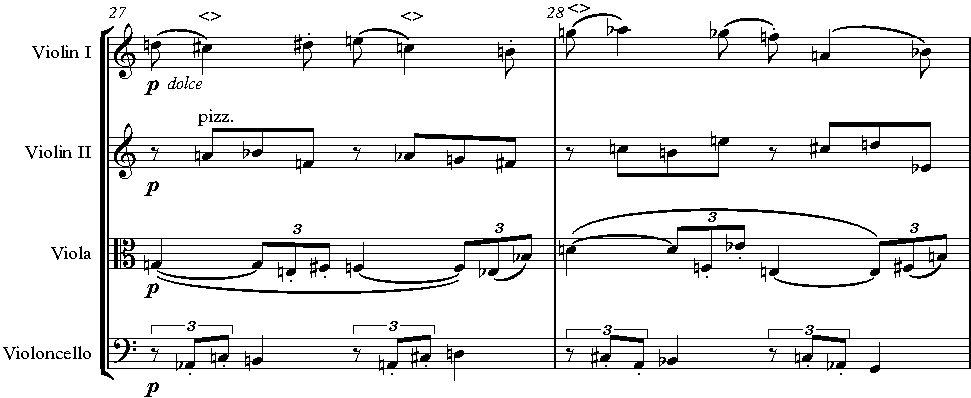
\includegraphics[width=6.5in]{figures/Schoenberg_4.pdf}
	\caption[Schoenberg's \emph{Fourth String Quartet} Op.~37]{Derived rows in Arnold Schoenberg's \emph{Fourth String Quartet} Op.~37 \cite[100]{Westergaard1966}.}
	\label{fig:schoenberg-quartet}
\end{figure}

%--------------------------------------------------------------------------
\noindent While separating the row between the two violins, two other rows are constructed, namely the row that is stated by the first violin between the two bars shown, and similarly the row that is stated by the second violin. These two rows are constructed from ordered segments extracted from the basic row, and so are said to be derived from it. Neither the first violin row, nor the second violin row are twelve-tone transforms of the original row or of each other. The same procedure of picking a fixed pattern of order numbers to separate the $[T_0 \; | \; T_5I]$ statement of the row between the two violins is used to split the $[T_5I \; | \; T_0]$ combined statement between viola and violoncello. While picking a fixed pattern of order numbers between the two lower instruments, however, the resulting linear statements for these instruments do not result in derived rows.

%--------------------------------------------------------------------------
Many structured approaches to derivation exist that guarantee that the extracted segments, when combined, will produce derived rows. These approaches often involve constructing a combination matrix of rows. The rows combined in the matrix are usually twelve-tone transforms of the same basic row. The rows that are derived from the segments of these transforms, on the other hand, may or may not be themselves transforms of the basic row.

%--------------------------------------------------------------------------
\begin{example}
The basic row in Berg's \emph{Lulu} may be used as motivation for a basic derivation procedure \cite[182]{Starr1984}. The first step is to create a $2 \times 24$ array where the first row $S$ is followed by $R(S)$, and the second row is initially undefined \cite[241]{Morris1977}.
\begin{equation}
    \left[
    \begin{array}{cccccccccccc|cccccccccccc}
    10 & 2 & 3 & 0 & 5 & 7 & 4 & 6 & 9 & 8 & 1 & 11 & 11 & 1 & 8 & 9 & 6 & 4 & 7 & 5 & 0 & 3 & 2 & 10 \\
    . & . & . & . & . & . & . & . & . & . & . & . & . & . & . & . & . & . & . & . & . & . & . & .
    \end{array}
    \right] \enspace.
\end{equation}
Next, an arbitrary segment is chosen, separated from the the top row, and placed in the bottom row.
\begin{equation}
    \left[
    \begin{array}{cccccccccccc|cccccccccccc}
    . & 2 & 3 & . & . & . & 4 & 6 & 9 & 8 & 1 & 11 & . & . & . & . & . & . & 7 & 5 & 0 & . & . & 10 \\
    10 & . & . & 0 & 5 & 7 & . & . & . & . & . & . & 11 & 1 & 8 & 9 & 6 & 4 & . & . & . & 3 & 2 & .
    \end{array}
    \right] \enspace.
\end{equation}
Let $V = \{ 2, 3, 4, 6, 9, 8, 1, 11, 7, 5, 0, 10 \}$. Then $V$ is a row derived from $S$. In particular, the ordered segment $\{ 10, 0, 5, 7 \}$ in $S$ is preserved by $R(V)$, and a counterpoint that combines $S$ vertically with $V$ horizontally is possible by construction.
\label{ex:derivation}
\end{example}

%--------------------------------------------------------------------------
\begin{figure}[htbp]
    \centering
	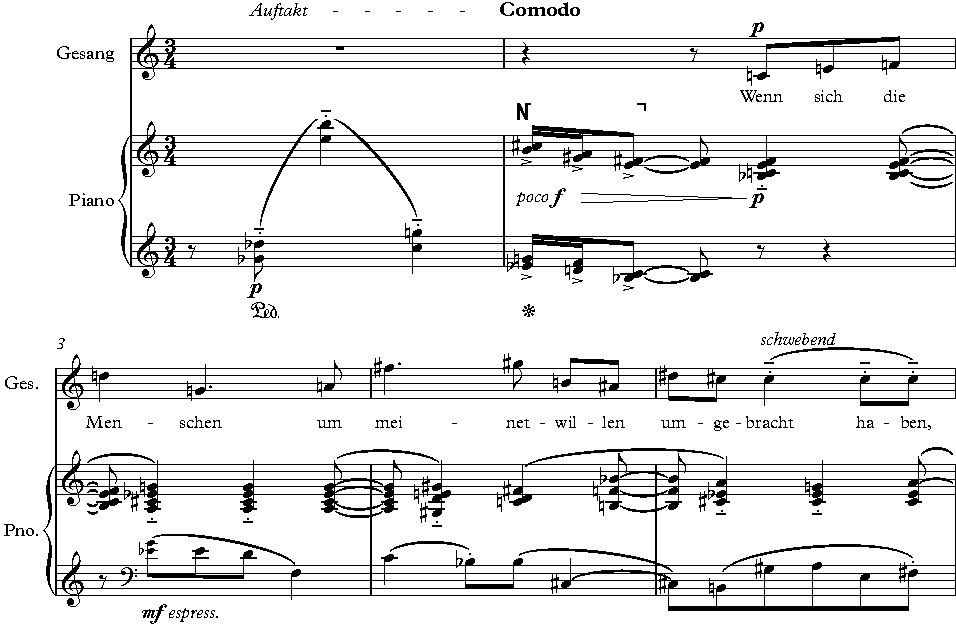
\includegraphics[width=6.5in]{figures/Berg_Lulu.pdf}
	\caption[Berg's \emph{Lied der Lulu}]{Alban Berg's \emph{Lied der Lulu} \cite[182]{Starr1984}.}
	\label{fig:berg-lulu}
\end{figure}

%--------------------------------------------------------------------------
It is of interest to note at this point that, in this kind of construction, the choice of a particular segment is already an important compositional decision. This choice bears relevance in that it establishes motivic material, that is, the segment itself. It also potentially introduces complementary harmonic regions, one given by the segment, the other given by its set complement. Moreover, and perhaps more importantly, it presents an opportunity for exploring syntax. There are a multitude of ways in which a composer may obtain syntax from a simple derivation procedure such as the one given in Ex.~\ref{ex:derivation}. One way would be to find an operation that makes the chosen segment invariant. In particular, it is easily checked that $S_1 = \{ 10, 0, 5, 7 \} = RT_5I(S_1)$. Ex.~\ref{ex:derivation} can then be followed by the combination matrix $[RT_5I(S) \; | \; T_5I(S_1)]$. In this second matrix, the segment $S_1$ could be preserved, but the row derived from $RT_5I(S)$ by preserving the segment $S_1$ would not be a transform of $V$. If the set complement of $S_1$ in $V$ were parsed to produce more than one harmonic region, then the complement of $S_1$ under this newly derived row would produce different harmonic regions under the same parsing. This procedure can be very pertinent compositionally, as it would be capable of producing contrasting harmonic regions while maintaining motivic coherence under the $S_1$ segment. Yet another way of generating syntax from derivation would be to follow $S$ with $V$ itself. A new row would then be derived from $V$, say $Q$, and eventually $V$ would be followed by $Q$. Repeating this procedure \emph{ad libitum} could generate many contrasting harmonic regions. In particular, this type of procedure is seen in Donald Martino's \emph{Notturno} of 1974, a composition that won the Pulitzer Prize in the following year \cite[181]{Starr1984}. If, by compositional choice, the same order numbers were always picked in the chain of derived rows, then a potential for rhythmic and agogic coherence could also be explored.

%--------------------------------------------------------------------------
\section{Literature Review}

%--------------------------------------------------------------------------
\enlargethispage{\baselineskip}
One of the earliest references in the academic literature of a procedure that may be construed as a derivation technique, illustrated below in Ex.~\ref{ex:martino-derivation}, is seen in \cite{Martino1961}, a paper whose main purpose is another, namely to generalize the construction of aggregate formations. The techniques described by Martino are influenced by Babbitt's ideas on combinatoriality \cite[224]{Martino1961}, and make extensive use of tables. In the interest of generalizing the construction of aggregate formations, Martino provides, in addition to hexachordal, also trichordal, tetrachordal, and even pentachordal combinatoriality tables, as well as somewhat brief discussions on oblique combinations \cite[241]{Martino1961}, which are further discussed in the context of derivation in \cite[216]{Starr1984}, and on uneven partitions of a row and their combinatoriality implications \cite[267]{Martino1961}. Martino acknowledges the aggregates formed by combinatoriality are not necessarily ordered, rather seeing this characteristic as capable of bringing harmonic diversity \cite[228, 230]{Martino1961}. In mentioning the derivation of new harmonic sets, this process is juxtaposed to another, namely the fragmentation of the original series. Both procedures are deemed to be essentially the same, since set derivation via aggregate formations can be seen as a fragmentation of the set obtained vertically \cite[230, 231]{Martino1961}.

%--------------------------------------------------------------------------
\begin{example}
	\label{ex:martino-derivation}
	\cite[231]{Martino1961}
	Let $S = \{ 0, 4, 11, 3, 1, 2, 5, 6, 9, 8, 10, 7 \}$ and consider the combination matrix $\hat{A}$.
	\begin{equation}
    	\hat{A} = [\hat{A}_1 | \hat{A}_2] = \left[
    	\begin{array}{cccccc|cccccc}
        	0 & 4 & 11 & 3 & 1 & 2 & 5 & 6 & 9 & 8 & 10 & 7 \\
        	7 & 10 & 8 & 9 & 6 & 5 & 2 & 1 & 3 & 11 & 4 & 0
    	\end{array}
    	\right] \enspace.
	\end{equation}
	In particular, the hexachords given by the $\hat{A}_i$ can be combined with their transforms under $T_1I$, yielding the combination matrix $A$.
	\begin{equation}
    	A = [A_1 | A_2 | A_3 | A_4] = \left[
    	\begin{array}{ccc|ccc|ccc|ccc}
        	0 & 4 & 11 & 3 & 1 & 2 & 5 & 6 & 9 & 8 & 10 & 7 \\
        	7 & 10 & 8 & 9 & 6 & 5 & 2 & 1 & 3 & 11 & 4 & 0 \\
        	\hline
        	1 & 9 & 2 & 10 & 0 & 11 & 8 & 7 & 4 & 5 & 3 & 6 \\
        	6 & 3 & 5 & 4 & 7 & 8 & 11 & 0 & 10 & 2 & 9 & 1
    	\end{array}
    	\right] \enspace.
	\end{equation}
	The row $Q = \{ 7, 0, 10, 6, 4, 1, 3, 5, 8, 9, 2, 11 \}$ can then be derived from the first column of $A$, but $T_9(Q)$ can only partially be derived from the second column of $A$, as pitch-classes 6 and 5 get swapped.
	\begin{equation}
        \left[
        \begin{array}{cccccccccccc|cccccccccccc}
            & 0 &&& 4 &&&&&&& 11 &&&& 3 & 1 &&& 2 &&&& \\
            7 && 10 &&&&&& 8 &&& && 9 &&&&&&& \boxed{6} & \boxed{5} && \\
            \hline
            &&&&& 1 &&&& 9 & 2 & &&&&&& 10 & 0 &&&& 11 & \\
            &&& 6 &&& 3 & 5 &&&& & 4 && 7 &&&&&&&&& 8
        \end{array}
        \right. \quad \cdots
    \end{equation}
\end{example}

%--------------------------------------------------------------------------
Even though the term derivation is not mentioned in \cite{Westergaard1966}, the paper introduces a mature conception of the problems involved with the technique of derivation. Two basic strategies for achieving polyphony from an essentially linear construct, namely partitioning and combining, are proposed \cite[95]{Westergaard1966}. Partitioning, which is illustrated in Fig.~\ref{fig:schoenberg-quartet}, consists of splitting a row into separate lines in a very Schenkerian fashion, with a bias toward partitioning the row in ways that preserve some of its intervallic structure \cite[100]{Westergaard1966}. Combining, on the other hand, departs from combination matrices, similarly to the technique demonstrated in Ex.~\ref{ex:martino-derivation}, and is truly remarkable in the sense that it already represents a technique for self-derivation \cite[101]{Westergaard1966}. Ex.~\ref{ex:westergaard} demonstrates the technique of combining.

%--------------------------------------------------------------------------
\enlargethispage{\baselineskip}
\begin{example}
	\label{ex:westergaard}
	\cite[102]{Westergaard1966}
	Let $S = \{ 2, 1, 9, 10, 5, 3, 4, 0, 8, 7, 6, 11 \}$ be a 12-tone row and consider the $12 \times 12$ matrix $A$.
	\begin{equation}
    	A = \left[
    	\begin{array}{cccccccccccc}
        	2 & 1 & 9 & 10 & 5 & 3 & 4 & 0 & 8 & 7 & 6 & 11 \\
        	1 & 0 & 8 & 9 & 4 & 2 & 3 & 11 & 7 & 6 & 5 & 10 \\
        	\vdots & \vdots & \vdots & \vdots & \vdots & \vdots & \vdots & \vdots & \vdots & \vdots & \vdots & \vdots \\
        	3 & 2 & 10 & 11 & 6 & 4 & 5 & 1 & 9 & 8 & 7 & 0
    	\end{array}
    	\right] \enspace.
	\end{equation}
	Then $\tilde{A}$ is a $12 \times 144$ combination matrix of self-derivation in which every column is a transform of $S$.
	\begin{equation}
    	\tilde{A} = \left[
    	\begin{array}{cccccccccccc|cccccccccccc|}
        	2 &&&&&&&&&&&    &  &&&&&&&& 1 &&& \\
        	& 1 &&&&&&&&&&   &  && 0 &&&&&&&&& \\
        	&&&&&&& 0 &&&&   &  &&& 11 &&&&&&&& \\
        	&&&&&&&&&&& 11   &  &&&&&&&&&&& 10 \\
        	&&& 10 &&&&&&&&  &  &&&&&&& 9 &&&& \\
        	&& 9 &&&&&&&&&   &  & 8 &&&&&&&&&& \\
        	&&&&&&&& 8 &&&   &  7 &&&&&&&&&&& \\
        	&&&&&&&&& 7 &&   &  &&&&& 6 &&&&&& \\
        	&&&&&&&&&& 6 &   &  &&&&&& 5 &&&&& \\
        	&&&& 5 &&&&&&&   &  &&&& 4 &&&&&&& \\
        	&&&&&& 4 &&&&&   &  &&&&&&&&&& 3 & \\
        	&&&&& 3 &&&&&&   &  &&&&&&&&& 2 &&
    	\end{array}
    	\; \quad \cdots \right. \enspace.
	\end{equation}
	The columns of $\tilde{A}$ are obtained by simply arranging the contents of each corresponding column of $A$. In particular, $\tilde{A} = [T_0(S) \; | \; T_5I(S) \; | \; \cdots$. Observing that 5 precedes 4 in the 10\textsuperscript{th} row of $\tilde{A}$, and similarly that 4 precedes 3 in the 11\textsuperscript{th} row of $\tilde{A}$, many alternative rearrangements of $\tilde{A}$ are possible, such as $\tilde{B}$.
	\pagebreak
	\begin{equation}
    	\tilde{B} = \left[
    	\begin{array}{cccccccccccc|cccccccccccc|}
        	2 &&&&&&&&&&&&&&&&&&&& 1 &&& \\
        	& 1 &&&&&&&&&&&&& 0 &&&&&&&&& \\
        	&& \vdots & \vdots &&&& \vdots & \vdots & \vdots & \vdots & \vdots & \vdots & \vdots && \vdots && \vdots & \vdots & \vdots &&&& \vdots \\
        	&&&& 5 && \boxed{4} &&&&&&&&&&&&&&&&& \\
        	&&&&&&&&&&&&&&&& \boxed{4} &&&&&& 3 & \\
        	&&&&& 3 &&&&&&&&&&&&&&&& 2 &&
    	\end{array}
    	\; \quad \cdots \right. \enspace.
    \end{equation}
    Combination matrices such as $A = [T_0 \; | \; \cdots \; | \; T_1]^T$ may be constructed in alternative ways where inverse and retrograde transforms of the row $S$ can be present. One possible sequence of transforms is
	\begin{equation}
		\{ T_0, T_{10}, T_{8}, T_{6}, T_{4}, T_{2}, T_{5}I, T_{3}I, T_{1}I, T_{11}I, T_{9}I, T_{7}I \} \enspace .
	\end{equation}
	Another is
	\begin{equation}
		\{ T_0, T_{8}, T_{4}, T_{11}I, T_{7}I, T_{3}I, RT_{9}, RT_{5}, RT_{1}, RT_{10}I, RT_{6}I, RT_{2}I \} \enspace .
	\end{equation}
\end{example}

%--------------------------------------------------------------------------
Self-derivation in $12 \times 144$ combination matrices is straightforward, since every column is capable of producing arbitrary transforms of any row. However, self-derivation in combination matrices of four rows or less is deemed more difficult to achieve \cite[108]{Westergaard1966}. Although a systematic way to understand self-derivation in smaller combination matrices is not proposed in \cite{Westergaard1966}, the advancements in the field are extremely substantial and arguably one strong motivating force for the studies in self-derivation that follow in the subsequent decades.

%--------------------------------------------------------------------------
In one of the seminal academic works in the field of twelve-tone theory, \cite{Starr1984} utilizes a mostly set-theoretic framework to understand and categorize rows and procedures involved in producing combination matrices of derivation and self-derivation. This approach revolves around the idea of looking at sets from the standpoint of their order constraints: a totally constrained set with no precedence contradictions is a twelve-tone row; a completely unconstrained set of twelve tones represents the free aggregate; each column of the matrix $A$ in Ex.~\ref{ex:westergaard} is a free aggregate; a maximally constrained set corresponds to the simultaneous aggregate, that is, a twelve-tone cluster. Sets that live in-between can often be projected in the middle and background of a composition, a fact that here too contributes to a Schenkerian view of the technique of derivation \cite[183, 184]{Starr1984}. Mathematically, the ideas in \cite{Starr1984} translate into considering the set $U$ of all ordered pairs of pitch-classes. There are twelve choices for the first position, and twelve choices for the second position. As both choices are independent, this set has cardinality $12^2 = 144$. An element of $U$ is called an order constraint, and a subset $C$ of $U$ is called a pitch-class relation. The latter can be viewed as a $12 \times 12$ matrix where the entry $c_{ij}$ is equal to one whenever $\{ i, j \} \in C$, and zero otherwise. Bitwise operations can be applied to these matrices in a very computationally efficient manner: bitwise \emph{and} and \emph{or} correspond respectively to set intersection and union. For any pair of pitch-classes $x$ and $y$, define a relation $x \sim y$ on the power set of $U$ by the set inclusion of the element $\{ x, y \}$. A subset $C$ will then be reflexive if, whenever an element of $C$ (which is a set) contains the pitch-class $x$, then $\{ x, x \} \in C$. In words, reflexivity means that if a reflexive collection $C$ of notes contains an element $x$, then $x$ precedes (and follows) itself in $C$. The free aggregate is a minimal reflexive subset of $U$ that contains all twelve tones. The relation $\sim$ will be symmetric if $\{ x, y \} \in C$ implies $\{ y, x \} \in C$, and antisymmetric whenever $\{ x, y \} \in C$ implies $\{ y, x \} \notin C$, for $x \ne y \in \mathbb{Z}/ 12 \mathbb{Z}$. Similarly, transitivity is defined as $\{ x, y \} \in C$ and $\{ y, z \} \in C$, then $\{ x, z\} \in C$; and trichotomy is defined as either $\{ x, y \} \in C$ or $\{ y, x \} \in C$ for any $x \ne y \in \mathbb{Z}/ 12 \mathbb{Z}$. The relation $\sim$ is, of course, an order relation on the set of twelve tones by definition. A partial order is one that is reflexive, transitive, and antisymmetric, while a total order (a row), is a partial order that satisfies trichotomy \cite[184, 185]{Starr1984}. Often, pitch-class relations will contain many redundancies due to transitivity. In order to express these relations as oriented graphs, such redundancies must first be removed, or pruned \cite[186]{Starr1984}. This process can be reversed and a pitch-class relation can be extended to the point of its transitive closure \cite[190]{Starr1984}. It is also common for a pitch-class relation to be absent of any order constraint involving both $\{ x, y \}$, in which case $x$ and $y$ are said to be incomparable. Such $x$ and $y$ are bound to be struck together, or else be linearized by the injection of some constraint that will make them comparable, as long as there still remains a partial order, that is, as long as this process does not introduce a symmetry, for instance. The set of all total orderings that can be linearized from some partial order is called its total order class \cite[188]{Starr1984}. In a completely analogous manner, a pitch-class relation can be can verticalized by removing constraints, and again minding that the result is still transitive and symmetric. A partial order covers another whenever the former is a verticalization of the latter. A simple procedure to guarantee that a verticalization will remain a partial order is to take its union with the free aggregate, then subject this union to an extension operation, thus providing reflexivity in the first step, as well as transitivity in the second \cite[192, 193]{Starr1984}. The following theorems provide more details on covering, as well as unions and intersections of pitch-class relations. In particular, Th.~\ref{starr-theorem} plays a crucial role in the construction of combination matrices of self-derivation from aggregate realizations \cite[222]{Starr1984}. Th.~\ref{starr-theorem-operations}, which is stated without proof, discusses aspects of applying twelve-tone operations to pitch-class relations.

%--------------------------------------------------------------------------
\begin{theorem}
    \cite[193]{Starr1984}
    \begin{enumerate}
        \item Covering is transitive;
        \vspace{-0.5em}
        \item A pitch-class relation is covered by its extension;
        \vspace{-0.5em}
        \item If a pitch-class relation covers another, then the extension of the former covers the extension of the latter.
    \end{enumerate}
\end{theorem}

%--------------------------------------------------------------------------
\begin{theorem}
    \cite[194]{Starr1984}
    \label{starr-theorem}
    Let $A$ and $B$ be partial orders and denote by $\Toc(A)$ and $\Toc(B)$ their respective total order classes. Then
    \begin{equation}
        \Toc(A) \cap \Toc(B) = \Toc(\Ext(A \cup B)) \enspace,
    \end{equation}
    where $\Ext$ is the extension operator. Moreover, if $A_i$ is a finite sequence of $n$ partial orders, then
    \begin{equation}
        \bigcap_{i = 0}^{n} \Toc(A_i) = \Toc \left[ \Ext\left ( \bigcup_{i = 0}^{n} A_i \right) \right] \enspace.
    \end{equation}
\end{theorem}

%--------------------------------------------------------------------------
\begin{theorem}
    \cite[194]{Starr1984}
    The intersection of two partial orders is again a partial order.
\end{theorem}

%--------------------------------------------------------------------------
\begin{theorem}
    \cite[195]{Starr1984}
    \label{starr-theorem-operations}
    Let $C$ be a pitch-class relation and $\{ a, b \}$ an element of $U$ such that $\{ a, b \} \in C$.
    \begin{enumerate}
        \item If $F$ is a pitch-class operation, then $\{ F(a), F(b) \} \in F(C)$ if and only if $\{ a, b \} \in C$. In particular, if $R(C)$ is the retrograde of $C$, then $\{ a, b \} \in R(C)$ if and only if $\{ b, a \} \in C$.
        \vspace{-0.5em}
        \item If $C$ is a totally ordered aggregate, then $R(C) = (S \setminus C) \cup \mathcal{F}$, where $S$ is the simultaneous aggregate and $\mathcal{F}$ is the free aggregate.
        \vspace{-0.5em}
        \item If $C_1$ covers $C_2$, then $F(C_1)$ covers $F(C_2)$.
        \vspace{-0.5em}
        \item Finally, if $C$ is $FR$-invariant, then all cycles in $F$ have length two.
    \end{enumerate}
\end{theorem}

%--------------------------------------------------------------------------
\enlargethispage{\baselineskip}
An aggregate realization is a particular type of partial order $C$ in which, for any pair of pitch-classes $a, b$, if $a$ and $b$ are incomparable in $C$, then the set of pitch-classes that precede $a$ in $C$ is equal to the set of pitch-classes that precede $b$ in $C$, and also the set of pitch-classes that follow $a$ in $C$ is equal to the set of pitch-classes that follow $b$ in $C$. Aggregate realizations arise naturally from a total order in the sense that they belong to the set of all partial orders that are covered by this total order, and lead to a classification of partial orders, as well as to many musical applications. One interesting compositional application of aggregate realizations is that of projecting a total order as a middle-ground entity. Given a sequence $S$ of partial orders, all of which are covered by the same total order, say $X$, if both $X$ is never stated in the foreground and $S$ contains all order constraints in $X$, then a musical passage in which $S$ is stated in the foreground will bear $X$ as a middle-ground entity. In the case where $S$ does not comprise all the order constraints in $X$, some other partial order that covers $S$ will be projected in the middle-ground. In the particular case where a composer is dealing with pitch-classes, projecting a partial order is equivalent to inducing the listener to infer its order constraints. If, in this case, two pitch-classes are incomparable, then they are bound to be struck together \cite[197]{Starr1984}. Fig.~\ref{fig:webern-variations} shows Webern's Op.~27 opening bars and Ex.~\ref{ex:webern-variations} illustrates how an aggregate realization may be obtained from the first four bars therein \cite[203, 204]{Starr1984}. Whereas aggregate realizations correspond to a totally ordered sequence of disjoint subsets of the free aggregate, a columnar aggregate is, on the other hand, a set of disjoint row segments where, even though the internal order of each segment is total, all segments are pairwise incomparable. In addition, a columnar aggregate must contain the free aggregate as a subset, so that all pitch-classes belonging to a given base are included in every column. The intersection of the set of all aggregate realizations with the set of all columnar realizations contains the set of all total orders (and thus all row segments), as well as the free aggregate. A total order is trivially an aggregate realization, and it is trivially a columnar realization. Any total order contains the free aggregate by the above \cite[201, 210]{Starr1984}.

%--------------------------------------------------------------------------
\enlargethispage{3em}
\begin{figure}[htbp]
    \centering
	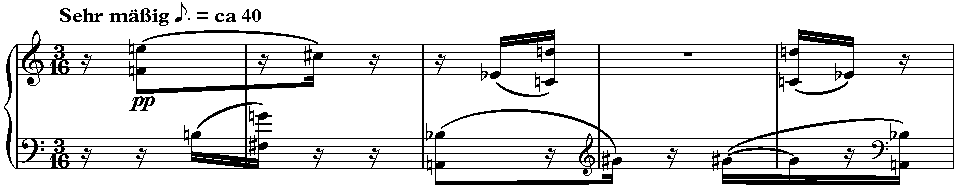
\includegraphics[width=6.5in]{figures/Webern_1.pdf}
	\caption[Webern's \emph{Variations for Piano} Op.~27]{Anton Webern's \emph{Variations for Piano} Op.~27 \cite[203]{Starr1984}.}
	\label{fig:webern-variations}
\end{figure}

%--------------------------------------------------------------------------
\begin{example}
    \cite[204]{Starr1984}
    \label{ex:webern-variations}
    Eq.~\ref{eq:webern-variations} shows an aggregate realization of Webern's Op.~27.
    \begin{equation}
    \label{eq:webern-variations}
    \begin{tikzcd}
		& E \arrow[dr] && G \arrow[dr] && B\flat \arrow[dr] && D \arrow[dr] & \\
		* \arrow[dr] \arrow[ur] && B \arrow[dr] \arrow[ur] && C\sharp \arrow[dr] \arrow[ur] && E\flat \arrow[dr] \arrow[ur] && G\sharp \\
		& F \arrow[ur] && F\sharp \arrow[ur] && A \arrow[ur] && C \arrow[ur] &
	\end{tikzcd}	
    \end{equation}
\end{example}

%--------------------------------------------------------------------------
A row segment is a pitch-class relation that is reflexive, transitive, and antisymmetric, with the additional requirement that some subset of its order constraints also satisfy trichotomy. Any partial order that covers some row segment is said to be an embedded segment of that partial order. By transitivity of covering, any other partial order covering the former partial order will have the aforementioned row segment embedded in it, including naturally any total order in its total order class. In this sense, a partial order may be seen as the union of its various embedded segments \cite[198]{Starr1984}. Row segments may be concatenated in a natural way. Let $X = \{ 0, 1, 2 \}$ and $Y = \{ 3, 4, 5 \}$ be row segments such that $X \cap Y = \emptyset$ when seeing $X$ and $Y$ as partial orders. The concatenation $X | Y$ will then be the partial order $X \cup Y \cup \{ \{ a, b \} : a \in X, b \in Y \}$. It follows both $X$ and $Y$ are embedded row segments of $X | Y$. The use of concatenation here is sequential, that is, the entire row segment $X$ precedes the entire row segment $Y$ in $X | Y$. In other words, intercalation of segments is not allowed when concatenating. Finding embedded segments that are common to different partial orders is straightforward. Let $X = \{ 0, 1, 7, 2, 10, 9, 11, 4, 8, 5, 3, 6 \}$ and $Y = \{ 1, 2, 8, 3, 11, 10, 0, 5, 9, 6, 4, 7 \}$ be total orders. In particular, $Y = T_1(X)$. Pruning the intersection $X \cap Y$ yields a graph whose longest row segments are $\{ 1, 2, 10, 9, 4 \}$, $\{ 1, 2, 10, 5, 6 \}$, $\{ 1, 2, 11, 5, 6 \}$, $\{ 1, 2, 8, 5, 6 \}$, and $\{ 1, 2, 8, 3, 6 \}$. These row segments are then the longest embedded segments of both $X$ and $Y$ \cite[200]{Starr1984}.

%--------------------------------------------------------------------------
Pruning an intersection of partial orders is also a method for computing common tones between sets that not only produces embedded segments, but can also be applied to the intersection of an arbitrary number of sets. When the sets are related to one another by a twelve-tone operation, finding common tones between them can be accomplished by expressing the operation as a permutation. Let $S = \{ 0, 1, 4, 5, 8, 9 \}$ and consider the cycle decomposition of $T_3I = (0 \; 3) \; (1 \; 2) \; (4 \; 11) \; (5 \; 10) \; (6 \; 9) \; (7 \; 8)$. It follows every pitch-class in $S$ maps to the twelve-tone complement of $S$ under $T_3I$. If the operation is $T_9 = (0 \; 9 \; 6 \; 3) \; (1 \; 10 \; 7 \; 4) \; (2 \; 11 \; 8 \; 5)$, then $S$ shares three common tones with $T_9(S)$, namely $0 \mapsto 9$, $4 \mapsto 1$, and $8 \mapsto 5$. A simple formula for computing the number of common tones between two sets under some $T_nI$ transform is also given in \cite[10]{Rahn1975}. Yet another technique for finding common tones between two sets consists of computing a table or matrix. This procedure has the advantage of not only giving all indices of transposition under which a set shares common tones with another, but of making it possible to determine whether these common tones will preserve their ordering after the transformation by examining the table's diagonals. It has the disadvantage of only being able to produce common tones between two sets at a time. Let $X$ be an 12-tone row seen as a column vector, and consider the $12 \times 12$ matrix $A = [X, \cdots, X]$. In particular, the matrix $B = A - A^T$ will have a main diagonal of zeros, which indicates that $X$ shares with itself 12 common tones under $T_0$. If there are $k$ threes in the matrix, then $X$ will share with itself $k$ tones under $T_3$. There is no requirement that a row be compared with itself. If, for instance, $A$ is given as above, and $\bar{A}$ is the matrix for the row $\bar{X}$, then counting the number $k$ of, say, threes in $B = A - \bar{A}^T$, will mean in turn that $X$ and $T_3(\bar{X})$ share $k$ tones under $T_3$. Naturally, the main diagonal of $B$ will not comprise only zeros if $A \ne \bar{A}$. To find common tones under inversion, let $B = A + A^T$ and, similarly, $M$ and $M \circ I$ become $B = A - M(A)^T$ and $B = A + M(A)^T$. Finally, if the indices being counted are disposed in any of the matrix's diagonals, then they will preserve ordering after the transform, thus becoming embedded segments; if, in addition, they are adjacent, then they will in fact be row segments shared by $X$ and the transform of $\bar{X}$ \cite[49]{Morris1987}. This matrix for finding common tones under transposition has the interesting property that it becomes a symmetric matrix when $A = \bar{A}$ and its elements are taken as interval classes. This reflects the fact that if $X$ shares $k$ tones with $T_i(X)$, then surely $T_i(X)$ will share exactly $k$ tones with $T_{12 - i}(X)$. If $i$ is an interval class, then $i = 12 - i$, showing why the matrix will be symmetric. The matrix of common tones under inversion is always symmetric, regardless whether its elements are taken as interval classes. Multiplicative operations, however, will often lack multiplicative inverses in twelve tones. For $p$-TET systems where $p$ is prime, multiplicative operations yield symmetric matrices as well, but those will sometimes require a proper definition of multiplicative interval classes.

%--------------------------------------------------------------------------
The procedure described in Ex.~\ref{ex:derivation} represents a type of derivation in which the series being displayed vertically is unrelated to the series being derived horizontally, except for the fact that both share a row segment when one of the rows is retrograded. The construction is part of a more general procedure, detailed in \cite[211]{Starr1984}, in which a row is always matched with a retrograded transform of itself. In the particular case of Ex.~\ref{ex:derivation}, the transform was $F = T_0$ for simplicity, but arbitrary twelve-tone operations may be used. Denote the given series by $S$ and define the derived row as $V = V_1 | V_2$, that is, $V$ is a concatenation of two row segments. The only requirement is that $V_1$, the segment that is singled out, remain invariant under $F$, which will force $V_2$ to also be invariant under $F$. In Ex.~\ref{ex:derivation} this requirement is satisfied trivially. It is usually the case in this type of derivation procedure that the invariance of $V$ under $F$, or under $R \circ F$ for that matter, does not preserve any ordering, as illustrated in Ex.~\ref{ex:derivation-unordered}. On the other hand, Ex.~\ref{ex:derivation-ordered} illustrates a derivation procedure similar to that in Ex.~\ref{ex:derivation} where the operation $F$ is not trivial and the singled-out segments are preserved as partial orders. That is accomplished by applying the technique described in \cite[49]{Morris1987} for finding common row segments. As a consequence of $F$ and the retrograde operation, combination matrices of this type feature two columns that are upside-down, $F$-mirrors of each other \cite[211]{Starr1984}. More can be said about such combination matrices. Prop.~\ref{derivation-polyphony-proposition} summarizes the general procedure under set-theoretic terms, and Eq.~\ref{eq:derivation-retrograde} provides the schematic representation of a derivation procedure involving the retrograde and an arbitrary operation $F$ \cite[212]{Starr1984}.

%--------------------------------------------------------------------------
\begin{proposition}
	\label{derivation-polyphony-proposition}
    \cite[211, 214]{Starr1984}
    Consider a 2-row combination matrix $C$ where a row is derived via the retrograde and some operation $F$. Denote the derived row by $V = V_1 | V_2$. Then the first column is the partial order $C_1 = V_1 \cup R \circ F(V_2)$, and similarly the second column is the partial order $C_2 = V_2 \cup R \circ F(V_1)$, such that $C_2 = R \circ F(C_1)$. If $D$ is a partial order that covers $C_1$, then $R \circ F(D)$ will cover $C_2$, and if $D$ is in the total order class of $C_1$, that is, $D$ is a row that can be linearized from $C_1$, then $R \circ F(D)$ is in the total order class of $C_2$. Finally, 2-row derivations of this type exist for arbitrary rows.
\end{proposition}

%--------------------------------------------------------------------------
\begin{equation}
\begin{array}{c|cc}
	\hline
    & S & R \circ F(S) \\
    \hline
    V & V_1 & V_2 \\
    R \circ F(V) & R \circ F(V_2) & R \circ F(V_1) \\
    \hline
\end{array}
\label{eq:derivation-retrograde}
\end{equation}

%--------------------------------------------------------------------------
\vspace{1em}
\begin{example}
    \cite[212]{Starr1984}
    \label{ex:derivation-unordered}
    Let $S = \{ 0, 1, 7, 2, 10, 9, 11, 4, 8, 5, 3, 6 \}$ and consider the operation $T_2I = (0 \; 2) \; (3 \; 11) \; (4 \; 10) \; (5 \; 9) \; (6 \; 8)$. Inspecting the cycle decomposition of $T_2I$ reveals that the segment $S_1 = \{ 0, 1, 7, 2 \}$ remains invariant under this operation. If a combination matrix involving $RT_2I$ is considered, however, then the segment $S_1$, seen as a partial order, shall not be preserved, since both $(1)$ and $(7)$ are fixed points. The same would happen to any $T_kI$ where $k$ is even. In particular, this shows that, in order to obtain the same ordered row segment in both columns of the combination matrix, $F$ cannot be trivial.
	\begin{equation}
    	\left[
    	\begin{array}{cccccccccccc|cccccccccccc}
        	0 & . & . & 1 & . & 7 & . & . & . & 2 & . & . & 10 & 9 & . & 11 & 4 & 8 & . & 5 & . & 3 & 6 & . \\
        	. & 8 & 11 & . & 9 & . & 6 & 10 & 3 & . & 5 & 4 & . & . & 0 & . & . & . & 7 & . & 1 & . & . & 2
    	\end{array}
    	\right] \enspace.
	\end{equation}
\end{example}

%--------------------------------------------------------------------------
\begin{example}
    \label{ex:derivation-ordered}
    Let $S = \{ 10, 2, 3, 0, 5, 7, 4, 6, 9, 8, 1, 11 \}$, the row in Berg's \emph{Lulu}, and consider the segment $\vec{s} = [10 \; 0 \; 5 \; 7]^T$ as a column vector. Now let $A^T = [\;\vec{s} \; | \; \vec{s} \; | \; \vec{s} \; | \; \vec{s}\;]$ be the square matrix whose every column is equal to $\vec{s}$. Then
	\begin{equation}
    	A + A^T = \begin{bmatrix}
    		2 & 10 & 3 & 5 \\
        	10 & 0 & 5 & 7 \\
        	3 & 5 & 10 & 0 \\
        	5 & 7 & 0 & 2
        \end{bmatrix} \pmod{12} \enspace.
	\end{equation}
	\noindent In particular, the row segment $\{ 10, 0, 5, 7 \}$ is invariant under $RT_5I$, since $A + A^T$ displays an anti-diagonal of fives. Thus, by matching $S$ with $RT_5I(S)$, the row segment $\{ 10, 0, 5, 7 \}$ may be obtained in the derived row $V$ itself, rather than in its retrograde, as was the case in Ex.~\ref{ex:derivation}. Setting it to $V_2$, say, yields $V = \{ 2, 3, 4, 6, 9, 8, 1, 11, 10, 0, 5, 7 \}$.
	\begin{equation}
    	\left[
    	\begin{array}{cccccccccccc|cccccccccccc}
        	. & 2 & 3 & . & . & . & 4 & 6 & 9 & 8 & 1 & 11 & . & . & . & . & . & . & 10 & 0 & 5 & . & . & 7 \\
        	10 & . & . & 0 & 5 & 7 & . & . & . & . & . & . & 6 & 4 & 9 & 8 & 11 & 1 & . & . & . & 2 & 3 & .
    	\end{array}
    	\right] \enspace.
	\end{equation}
\end{example}

%--------------------------------------------------------------------------
A distinction is made in \cite[211, 214]{Starr1984} between derivation and polyphonyzation. The former departs from a combination matrix of rows to infer a concatenation of rows that constitute the linearized result of flattening the combination matrix. The latter is the opposite concept, that is, given a concatenation of rows, a combination matrix is constructed such that each column breaks down the row at the top into disjoint ordered segments. Although differentiating between derivation and polyphonization is an important concept in the set-theoretic view of the problem, this paper shall not make that distinction. The term derivation will be used indiscriminately to both the breaking down of rows into contrapuntal combination matrices, and the flattening thereof.

%--------------------------------------------------------------------------
A related technique involving greater than 2-row counterpoint is achieved by folding a combination matrix. The process is similar to first constructing a matrix of hexachordal combinatoriality in the traditional sense, then deriving rows from this matrix using the techniques above. Let $S$ be a row whose first hexachord is invariant under the operation $G$. Consider a row $V = V_1 | V_2$ and an operation $F$ such that $S$ is in the total order class of $V_1 \cup R \circ F(V_2)$. Then putting $S$ in counterpoint with $G(S)$, as well as deriving $V$ from $S | R \circ F(S)$, yields the schematic representation in Eq.~\ref{eq:derivation-folded}. It is argued without proof that vertically satisfying $G$ while horizontally satisfying $F$ implies $F$ and $G$ must commute \cite[215]{Starr1984}. Ex.~\ref{ex:derivation-folded} shows an application of folded derivation.

%--------------------------------------------------------------------------
\pagebreak
\begin{equation}
\begin{array}{c|cc}
	\hline
	& S & R \circ F(S) \\
	\hline
	V & V_1 & V_2 \\
	R \circ F(V) & R \circ F(V_2) & R \circ F(V_1) \\
	R \circ GF(V) & R \circ GF(V_2) & R \circ GF(V_1) \\
	G(V) & G(V_1) & G(V_2) \\
	\hline
	& G(S) & R \circ GF(S) = R \circ FG(S) \\
	\hline 
\end{array}
\label{eq:derivation-folded}
\end{equation}

%--------------------------------------------------------------------------
\vspace{1em}
\begin{example}
    \cite[215]{Starr1984}
    \label{ex:derivation-folded}
    Let $S = \{ 0, 1, 11, 3, 8, 10, 4, 9, 7, 6, 2, 5 \}$ and consider the cycle decomposition of $T_6 = (0 \; 6) \; (1 \; 7) \; (2 \; 8) \; (3 \; 9) \; (4 \; 10) \; (5 \; 11)$. Let $V_1 = \{ 1, 3, 8, 9, 7, 2 \}$. Since the unordered set $V_1$ is $T_6$-invariant, it follows $V_2 = \{ 11, 0, 10, 4, 5, 6 \}$ and the following combination matrix is obtained:
    \begin{equation}
        \left[
        \begin{array}{cccccccccccc|cccccccccccc}
            & 1 && 3 & 8 &&& 9 & 7 && 2 && 11 && 0 &&& 10 & 4 &&& 5 && 6 \\
            0 && 11 &&& 10 & 4 &&& 6 && 5 && 8 && 1 & 3 &&& 2 & 9 && 7 &  
        \end{array}
        \right] \enspace.
    \end{equation}
    Consider further the cycle decomposition of $T_5I = (0 \; 5) \; (1 \; 4) \; (2 \; 3) \; (6 \; 11) \; (7 \; 10) \; (8 \; 9)$. Then $S_1 = \{ 0, 1, 11, 3, 8, 10 \}$ maps to its complement under $T_5I$, so $S$ can be used in a combination matrix where $S$ is matched with its transform under $T_5I$ in the usual way, that is, in a matrix of hexachordal combinatoriality. Moreover, the row $T_5I(V)$ can be derived from $T_5I(S)$. Since $T_5I$ commutes with $T_6$, as any pitch-class operation does, the following folded derivation is possible:
    \begin{equation}
        \left[
        \begin{array}{cccccccccccc|cccccccccccc}
            & 1 && 3 & 8 &&& 9 & 7 && 2 && 11 && 0 &&& 10 & 4 &&& 5 && 6 \\
            0 && 11 &&& 10 & 4 &&& 6 && 5 && 8 && 1 & 3 &&& 2 & 9 && 7 & \\
            \hline
            5 && 6 &&& 7 & 1 &&& 11 && 0 && 9 && 4 & 2 &&& 3 & 8 && 10 & \\
            & 4 && 2 & 9 &&& 8 & 10 && 3 && 6 && 5 &&& 7 & 1 &&& 0 && 11
        \end{array}
        \right] \enspace.
    \end{equation}
\end{example}

%--------------------------------------------------------------------------
\pagebreak
An analogue to the technique of oblique combination described in \cite[241, 267]{Martino1961} is given in \cite{Starr1984} in the context of folded derivation, and denoted skewed polyphonization. The procedure consists of shifting horizontally one of the two rows of the derivation matrix. Skewed polyphonization may be equivalent to folding combination matrices that involve the retrograde, and there is no requirement that the combinatoriality be hexachordal. Eq.~\ref{eq:derivation-shifted} provides a schematic description of a skewed polyphonization procedure involving the retrograde. The asterisk indicates there is no requirement that the same row class be derived in both foldings, in which case $V$ would be replaced by some other row $V^*$ and $G$ could be the identity. An interesting compositional application consists of matching altogether different foldings of a row, thus effectively bridging different derivations of the same generative material. Ex.~\ref{ex:derivation-shifted} shows an application of skewed polyphonization where combinatoriality is not hexachordal, but both foldings derive different transforms of the same row \cite[216]{Starr1984}.

%--------------------------------------------------------------------------
\begin{equation}
\begin{array}{c|ccc}
	\hline
    & S & R \circ F(S) & \\
    \hline
    V & V_1 & V_2 & \\
    R \circ F(V) & R \circ F(V_2) & R \circ F(V_1) & \\
    R \circ G(V)^* && R \circ G(V_2)^* & R \circ G(V_1)^* \\
    GF(V)^* && GF(V_1)^* & GF(V_2)^* \\
    \hline
    && GF(S) & R \circ G(S) \\
    \hline
\end{array}
\label{eq:derivation-shifted}
\end{equation}

%--------------------------------------------------------------------------
\vspace{1em}
\begin{example}
    \cite[216]{Starr1984}
    \label{ex:derivation-shifted}
    Consider the row $S = \{ 0, 1, 7, 2, 10, 9, 11, 4, 8, 5, 3, 6 \}$ and the combination matrix given by $RT_{10}I(S)$ against $T_{11}(S)$:
    \begin{equation}
        \left[
        \begin{array}{cccccccc|cccccccc}
            4 && 7 && 5 && 2 && 6 & 11 & 1 & 0 & 8 & 3 & 9 & 10 \\
            11 & 0 & 6 & 1 & 9 & 8 & 10 & 3 && 7 && 4 && 3 && 5
        \end{array}
        \right] \enspace.
    \end{equation}
    Deriving the row $V = V_1 | V_2 = \{ 1, 7, 2, 9, 8, 3 \} | \{ 4, 5, 6, 11, 0, 10 \}$ from $S | RT_{10}I(S)$, and following the scheme given in Eq.~\ref{eq:derivation-shifted}, yields the following shifted derivation:
    \pagebreak
    \begin{equation*}
        \left[
        \begin{array}{cccccccccccc|cccccccc|c}
            & 1 & 7 & 2 && 9 &&& 8 && 3 && 4 &&&& 5 &&&& 6 \\
            0 &&&& 10 && 11 & 4 && 5 && 6 & && 7 &&&& 2 && \\
            \hline
            &&&&&&&&&&&& & 0 & 6 & 1 && 8 &&& 7 \\
            &&&&&&&&&&&& 11 &&&& 9 && 10 & 3 &
        \end{array}
        \right. \quad \cdots
    \end{equation*}
    \begin{equation}
        \cdots \quad \left. \begin{array}{c|cccccccc|cccccccccccc}
            & 6 & 11 && 0 &&&& 10 &&&&&&&&&&& \\
            & && 1 && 8 & 3 & 9 & &&&&&&&&&&& \\
            \hline
            & 7 &&&& 3 &&& & 3 && 4 && 5 & 10 && 11 &&&& 9 \\
            3 &&& 4 &&&& 5 & && 6 && 1 &&& 0 && 7 & 2 & 8
        \end{array} \right] \enspace.
    \end{equation}
\end{example}

%--------------------------------------------------------------------------
\vspace{1em}
Self-derivation is discussed in \cite[217, 226]{Starr1984} both from the set-theoretic perspective, and from the standpoint of aggregate realizations. The only difference between self-derivation and the general case is that, in combination matrices of self-derivation, all row forms belong to the same row class, that is, all rows are $RT_nI$ transforms of the original row. The same applies to folded and skewed combination matrices of self-derivation. The general scheme for a two-row combination matrix of self-derivation involving the retrograde is given in Eq.~\ref{eq:derivation-self} \cite[219]{Starr1984}. It is stated without proof in \cite[217]{Starr1984} that the operations $F$ and $G$ in Eq.~\ref{eq:derivation-self} must commute. For this type of self-derivation on two-row counterpoint, however, simple inspection of the examples that follow such statement already affords a counter-proof, as described in Ex.~\ref{topSquareSideExample}. Similarly to the general derivation case, two-row self-derivations can also be folded. Although the same term is used, folding in combination matrices of self-derivation usually means taking one of the derived rows and pulling another level of self-derivation from it, as seen in Ex.~\ref{self-folded}. The problem size grows as a natural consequence of folding combination matrices of self-derivation. The folded rows can subsequently be folded, and this procedure can generate many levels of self-derivation \cite[221]{Starr1984}. Ex.~\ref{ex:scotto} provides a musical application of folded self-derivation matrices that constitute a fundamental compositional procedure in Ciro Scotto's \emph{Tetralogy}. Folded self-derivation matrices are discussed in detail by Kowalski in \cite{Kowalski1987a}, always in the context of Eq.~\ref{eq:self-third} and not as the technique described in Ex.~\ref{ex:derivation-folded}.

%--------------------------------------------------------------------------
\begin{equation}
\begin{array}{c|cc}
	\hline
    & G(S) & R \circ FG(S) \\
    \hline
    S & S_1 & S_2 \\
    R \circ F(S) & R \circ F(S_2) & R \circ F(S_1) \\
    \hline
\end{array}
\label{eq:derivation-self}
\end{equation}

%--------------------------------------------------------------------------
\vspace{1em}
\begin{example}
	\label{topSquareSideExample}
    \cite[218]{Starr1984}
    Let $S = S_1 | S_2 = \{ 3, 8, 1, 0, 9, 6 \} | \{ 4, 7, 10, 5, 2, 11 \}$ and consider the cycle decomposition of $T_9I = (0 \; 9) \; (1 \; 8) \; (2 \; 7) \; (3 \; 6) \; (4 \; 5) \; (10 \; 11)$. In particular, both $S_1$ and $S_2$ are invariant under $T_9I$. It is not obvious, however, that $S$ and $RT_9I(S)$ can be derived from a combination matrix $A$ where the first column is $T_7(S)$ and the second is $RT_2I(S) = RT_9I \circ T_7(S)$. Here $F = T_9I$ and $G = T_7$. It is not the case that $F$ and $G$ commute, as $T_2I = F \circ G \ne G \circ F = T_4I$.
    \begin{equation}
    	\label{topSquareSideEquation}
        A = \left[
        \begin{array}{cccccccccccc|cccccccccccc}
            & 3 & 8 &&& 1 &&&& 0 & 9 & 6 &&&& 4 & 7 & 10 && 5 & 2 &&& 11 \\
            10 &&& 7 & 4 && 11 & 2 & 5 &&&& 3 & 0 & 9 &&&& 8 &&& 1 & 6 &
        \end{array}
        \right] \enspace.
    \end{equation}
\end{example}

%--------------------------------------------------------------------------
\begin{example}
    \cite[221]{Starr1984}
    \label{self-folded}
    Let $S = \{ 0, 11, 5, 10, 4, 2, 7, 9, 8, 3, 6, 1 \}$ and consider the following combination matrix given by $T_2(S) | RT_2(S)$, whose derived rows are $S$ and $R(S)$:
    \begin{equation}
        \label{eq:self-first}
        \left[
        \begin{array}{cccccccccccc|cccccccccccc}
            & 0 && 11 & 5 &&& 10 && 4 && 2 && 7 && 9 && 8 & 3 &&& 6 && 1 \\
            1 && 6 &&& 3 & 8 && 9 && 7 && 2 && 4 && 10 &&& 5 & 11 && 0 &
        \end{array}
        \right] \enspace.
    \end{equation}
    Subjecting the entire matrix to $T_1$ yields:
    \begin{equation}
        \label{eq:self-second}
        \left[
        \begin{array}{cccccccccccc|cccccccccccc}
            & 1 && 0 & 6 &&& 11 && 5 && 3 && 8 && 10 && 9 & 4 &&& 7 && 2 \\
            2 && 7 &&& 4 & 9 && 10 && 8 && 3 && 5 && 11 &&& 6 & 0 && 1 &
        \end{array}
        \right] \enspace.
    \end{equation}
    The entire matrix in Eq.~\ref{eq:self-first} can then be pulled from the first row of Eq.~\ref{eq:self-second}:
    \begin{equation}
    	\label{eq:self-third}
        \left[
        \begin{array}{cccccccccccc|cccccccccccc|c}
            &&& 0 &&&& 11 && 5 &&&&&& 10 &&& 4 &&&&& 2 & \\
            & 1 &&& 6 &&&&&&& 3 && 8 &&&& 9 &&&& 7 &&& 2 \\
            2 && 7 &&& 4 & 9 && 10 && 8 && 3 && 5 && 11 &&& 6 & 0 && 1 &&
        \end{array}
        \quad \cdots \right. \enspace.
    \end{equation}
\end{example}

%--------------------------------------------------------------------------
\begin{example}
    \label{ex:scotto}
    Let $S = \{ 0, 4, 7, 3, 11, 2, 10, 1, 6, 8, 9, 5 \}$ and consider the self-deriving combination matrix given by Eq.~\ref{eq:scotto-1}. In it, the columns are $[T_0 \; | \; RT_0]$, and the derived rows are $[T_7 \; | \; RT_7]^T$ \cite[179]{Scotto2000}.
    \begin{equation}
        \label{eq:scotto-1}
        \left[
        \begin{array}{cccccccccccc|cccccccccccc}
            && 7 && 11 & 2 & 10 && 6 && 9 && 5 && 8 && 1 &&&& 3 && 4 & 0 \\
            0 & 4 && 3 &&&& 1 && 8 && 5 && 9 && 6 && 10 & 2 & 11 && 7 &&
        \end{array}
        \right] \enspace.
    \end{equation}
	\noindent Similarly to Ex.~\ref{self-folded}, the above matrix can be folded in order to obtain subsequent levels of derivation. Unlike Ex.~\ref{self-folded}, however, Scotto derives a rotated transform of $S$ from $RT_7(S)$. The rows in Eq.~\ref{eq:scotto-folded} are thus $T_2(S), RT_2(S), \rho_6RT_2(S)$ and $\rho_6T_2(S)$, where $\rho$ is the cyclical rotation operator \cite[180]{Scotto2000}.
	\begin{equation*}
		\label{eq:scotto-folded}
        \left[
        \begin{array}{cccccccccccc|cccccccccccc|}
        	&&&&& 2 &&& 6 && 9 && 5 &&&& 1 &&&&&& 4 & \\
        	&& 7 && 11 && 10 &&&&&&&& 8 &&&&&& 3 &&& 0 \\
        	\hline
        	& 4 &&&&&& 1 &&&& 5 && 9 && 6 &&& 2 &&&&& \\
        	0 &&& 3 &&&&&& 8 &&&&&&&& 10 && 11 && 7 &&
        \end{array}
        \right. \quad \cdots
    \end{equation*}
	\begin{equation}
        \cdots \quad \left.
        \begin{array}{|cccccccccccc|cccccccccccc}
        	0 &&& 3 &&&&&& 8 &&&&&&&& 10 && 11 && 7 && \\
        	& 4 &&&&&& 1 &&&& 5 && 9 && 6 &&& 2 &&&&& \\
        	\hline
        	&& 7 && 11 && 10 &&&&&&&& 8 &&&&&& 3 &&& 0 \\
        	&&&&& 2 &&& 6 && 9 && 5 &&&& 1 &&&&&& 4 &
        \end{array}
        \right] \enspace.
    \end{equation}
    \newpage
    \noindent In an entirely Schenkerian fashion, Scotto utilizes the folded matrix as the source material for a high-level structure in \emph{Tetralogy}. The only difference between the derivation matrix and the Schenkerian graph is that $T_2(S)$ now corresponds to the alto register, as seen in Fig.~\ref{fig:scotto-schenker1}. Rather than a strict serial composition, \emph{Tetralogy} employs a variety of prolongation procedures which are in line with its Schenkerian orientation \cite[179, 181]{Scotto2000}. Fig.~\ref{fig:scotto-music1} shows a musical realization containing the soprano and bass voices in the high-level structure \cite[204]{Scotto2000}.
	\begin{figure}[H]
    	\centering
		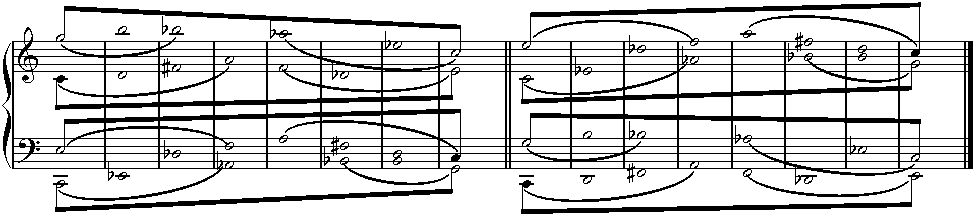
\includegraphics[width=6.5in]{figures/Scotto_Schenker_1.pdf}
		\caption[Schenkerian high-level structure in Scotto's \emph{Tetralogy}]{Schenkerian high-level structure in Scotto's \emph{Tetralogy} \cite[181]{Scotto2000}.}
    	\label{fig:scotto-schenker1}
	\end{figure}
	\begin{figure}[H]
    	\centering
    	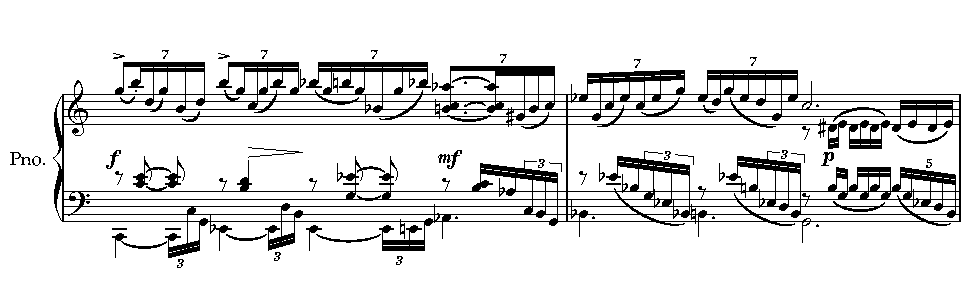
\includegraphics[width=6.5in]{figures/Scotto_1.pdf}
		\caption[Musical realization of the high-level structure in Scotto's \emph{Tetralogy}]{Realization of the high-level structure in Scotto's \emph{Tetralogy} \cite[205]{Scotto2000}.}
    	\label{fig:scotto-music1}
	\end{figure}
\end{example}

%--------------------------------------------------------------------------
Three algorithms for computing combination matrices of self-derivation are presented in \cite{Starr1984}. The first is an algorithm for computing $2 \times 24$ matrices that consists of finding a segment at the beginning of an ordered set that can become an embedded segment in some transform of the set, then constructing a combination matrix involving the retrograde by manually resolving any symmetries. There is no prior knowledge of the entire row, thus the row is actually composed by adding order constraints to an initially unconstrained set \cite[217]{Starr1984}. The second algorithm utilizes Th.~\ref{starr-theorem} to construct self-derivation from columnar aggregates by finding operations that resolve symmetries between the columns of the matrix. Although there is no requirement that the matrix be retrograde-invariant, the retrograde makes it arguably easier to work out the algorithm by hand. Ex.~\ref{ex:starr-algorithm-2} illustrates the second algorithm in which, similarly to the first, the entire row is discovered as a result of the procedure \cite[222]{Starr1984}. The third algorithm proposed makes use of aggregate realizations to compose combination matrices of self-derivation, and also utilizes Th.~\ref{starr-theorem}. Ex.~\ref{ex:starr-aggregate-realization} illustrates how this third algorithm works by explicitly building the aggregate realizations in the matrix from the cycles of some operation \cite[226, 227]{Starr1984}, and Ex.~\ref{ex:stingray} shows how a $6 \times 72$ matrix of self-derivation may be used in a musical composition. This matrix was constructed by exploring the symmetries of an aggregate realization, that is, by using the third algorithm described in \cite{Starr1984}.

%--------------------------------------------------------------------------
\pagebreak
\begin{example}
	\cite[224]{Starr1984}
	\label{ex:starr-algorithm-2}
    Let $S = \{ 0, 1, 7, 2 \} | \{ 10, 9 \} | \{ 11, 4, 8, 5 \} | \{ 3, 6 \}$. Given that the complement of a row's first hexachord is always obtained from its second hexachord, a trivial case of hexachordal combinatoriality results when a row is matched with its retrograde. It is then possible to partition $S$ such that the combination matrix will have four columns:
    \begin{equation}
        A = \left[
        \begin{array}{c|c|c|c}
        	\{ 0, 1, 7, 2 \} & \{ 10, 9 \} & \{ 11, 4, 8, 5 \} & \{ 3, 6 \} \\
        	\{ 6, 3 \} & \{ 5, 8, 4, 11 \} & \{ 9, 10 \} & \{ 2, 7, 1, 0 \}
        \end{array}
        \right] \enspace.
    \end{equation}
    Now consider the cycles of $T_{11}I = (0 \; 11) \; (1 \; 10) \; (2 \; 9) \; (3 \; 8) \; (4 \; 7) \; (5 \; 6)$. In particular, the first column of $A$ will comprise the partial order $S_1 \cup R(S_4)$, and this union will, in turn, map onto its hexachordal complement under $T_{11}I$, as it takes precisely one element from each of the operation's cycles, all of which have length two. Since the second column above is the complement of the first, it will also map onto its complement under $T_{11}I$. Because the third and fourth columns are mirrors of the first two, hexachordal combinatoriality under $T_{11}I$ is obtained in every column, that is, for the partial orders $S_1 \cup R(S_4)$ and $S_2 \cup R(S_3)$, as well as their retrogrades. The same result is not obtained between $S$ and $T_{11}I(S)$, that is, the first hexachord of $T_{11}I(S)$ is \emph{not} the complement of the first hexachord of $S$. This procedure yields the matrix $\hat{A}$.
    \begin{equation}
        \hat{A} = \left[
        \begin{array}{c|c|c|c}
        	\{ 0, 1, 7, 2 \} & \{ 10, 9 \} & \{ 11, 4, 8, 5 \} & \{ 3, 6 \} \\
        	\{ 6, 3 \} & \{ 5, 8, 4, 11 \} & \{ 9, 10 \} & \{ 2, 7, 1, 0 \} \\
        	\{ 11, 10, 4, 9 \} & \{ 1, 2 \} & \{ 0, 7, 3, 6 \} & \{ 8, 5 \} \\
        	\{ 5, 8 \} & \{ 6, 3, 7, 0 \} & \{ 2, 1 \} & \{ 9, 4, 10, 11 \}
        \end{array}
        \right] \enspace.
    \end{equation}
    The above can be construed as a sequence of four columnar aggregates. It may be possible to derive members of the same row class from each column. If the total order class of the intersection of all columns is not empty, that is, if it contains the free aggregate and does not contain any symmetry, then Th.~\ref{starr-theorem} guarantees that representatives of this row class can be derived from each column. Let $C_1, C_2, C_3, C_4$ be the four columns of the matrix $\hat{A}$. It follows the row $V = \{ 11, 0, 1, 6, 10, 4, 7, 2, 9, 5, 3, 8 \}$ has the property that $T \in \Toc \{ \Ext[ C_1 \cup RT_1I(C_2) \cup T_1I(C_3) \cup R(C_4) ] \}$. Therefore $[V | RT_1I(V) | T_1I(V) | R(V)]$ can be derived from the columns of $\hat{A}$.
    \begin{equation*}
        \left[
        \begin{array}{cccccccccccc|cccccccccccc|}
            & 0 & 1 &&&& 7 & 2 &&&& && 10 &&&&& 9 &&&&& \\
            &&& 6 &&&&&&& 3 & & 5 && 8 & 4 & 11 &&&&&&& \\
            \hline
            11 &&&& 10 & 4 &&& 9 &&& &&&&&&&&&&& 1 & 2 \\
            &&&&&&&&& 5 && 8 &&&&&& 6 && 3 & 7 & 0 &&
        \end{array}
        \right. \quad \cdots
    \end{equation*}
    \begin{equation}
        \cdots \left. \quad
        \begin{array}{|cccccccccccc|cccccccccccc}
            &&&&&&& 11 & 4 & 8 && 5 && 3 &&&&&&& 6 &&& \\
            &&&&& 9 &&&&& 10 & &&&&& 2 & 7 &&&& 1 & 0 & \\
            \hline
            && 0 & 7 & 3 && 6 &&&&& & 8 && 5 &&&&&&&&& \\
            2 & 1 &&&&&&&&&& &&&& 9 &&& 4 & 10 &&&& 11
        \end{array} \right] \enspace.
    \end{equation}
\end{example}

%--------------------------------------------------------------------------
\begin{example}
    \cite[226, 227]{Starr1984}
    \label{ex:starr-aggregate-realization}
    Let
    \begin{equation}
    	S = S_1 \; | \; S_2 \; | \; S_3 = \{ 0, 1, 7, 2 \} \; | \; \{ 10, 9, 11, 4 \} \; | \; \{ 8, 5, 3, 6 \}
    \end{equation}
    and consider the matrix $A = [S \; | \; T_4(S) \; | \; T_8(S)]^T$.
    \begin{equation}
        A = \left[
        \begin{array}{cccc|cccc|cccc}
        	0 & 1 & 7 & 2 & 10 & 9 & 11 & 4 & 8 & 5 & 3 & 6 \\
        	4 & 5 & 11 & 6 & 2 & 1 & 3 & 8 & 0 & 9 & 7 & 10 \\
        	8 & 9 & 3 & 10 & 6 & 5 & 7 & 0 & 4 & 1 & 11 & 2
        \end{array}
        \right] \enspace.
    \end{equation}
    Now let $V$ be in the total order class of the first columnar aggregate of $A$. Next, rewrite the first columnar aggregate of $A$ as the aggregate realization $A_1$.
    \begin{equation}
        A_1 = \begin{tikzcd}
            & 0 \arrow[dr] && 1 \arrow[dr] && 7 \arrow[dr] && 2 \arrow[dr] & \\
            * \arrow[r] \arrow[dr] \arrow[ur] & 4 \arrow[r] & * \arrow[r] \arrow[dr] \arrow[ur] & 5 \arrow[r] & * \arrow[r] \arrow[dr] \arrow[ur] & 11 \arrow[r] & * \arrow[r] \arrow[dr] \arrow[ur] & 6 \arrow[r] & * \\
            & 8 \arrow[ur] && 9 \arrow[ur] && 3 \arrow[ur] && 10 \arrow[ur] &
        \end{tikzcd}
    \end{equation}
    When the first column of $A$ is regarded as an aggregate realization, it becomes clearer that any $V \in \Toc(A_1)$ must be a succession of augmented triads. One possibility would be $V = \{ 4, 8, 0, 9, 1, 5, 11, 7, 3, 2, 10, 6 \}$. It is easy to see that linearizing $V$ from $A_1$ is possible, but it is not obvious whether some transform of $V$ can be linearized from the other columns of $A$. The answer depends on the chosen operation, $T_4$ in this case, and on the chosen $S$. To verify that $A_2$ is a transform of $A_1$, it suffices to check whether there is a base-four $RT_nMI$ operation that maps $S_1 \pmod 4$ onto $S_2 \pmod 4$. This is easily verified, as indeed
    \begin{equation}
        S_1 \pmod 4 = \{ 0, 1, 3, 2 \} = T_2I(\{ 2, 1, 3, 0 \}) = T_2I \circ S_2 \pmod 4 \enspace.
    \end{equation}
    The above method works because the elements in each of $A_1$'s columns are incomparable, thus may be picked from each column in any order. In other words, $A_1$ could be flipped horizontally, say, and still have the same aggregate realization. Since all of $A$'s columns can be reduced $\pmod 4$ by construction, it becomes enough to only consider each column's residue modulo four, and four-tone operations. Since $S_1 \pmod 4 = S_3 \pmod 4$, $V$ itself can be derived from $A_3$, yielding the following derivation matrix, where the second column is $T_2I(V)$:
    \begin{equation*}
        \left[
        \begin{array}{cccccccccccc|cccccc}
        	&& 0 && 1 &&& 7 && 2 && & 10 &&&&& 9 \\
        	4 &&&&& 5 & 11 &&&&& 6 & && 2 && 1 & \\
        	& 8 && 9 &&&&& 3 && 10 & & & 6 && 5 &&
        \end{array}
        \right. \quad \cdots
    \end{equation*}
    \begin{equation}
        \cdots \left. \quad
        \begin{array}{cccccc|cccccccccccc}
        	&& 11 && 4 & & & 8 &&&& 5 &&& 3 &&& 6 \\
        	3 &&&&& 8 & && 0 & 9 &&&& 7 &&& 10 & \\
        	& 7 && 0 && & 4 &&&& 1 && 11 &&& 2 &&
        \end{array}
        \right] \enspace.
    \end{equation}
    It may be possible to derive other rows from $A$ that are not based on the concatenation of cycles from an operation. Knowing that the columns of $A$ are related as aggregate realizations by the operation tuple $\mathcal{A} = [T_0 \; T_2I \; T_0]$, and regarding the $A_i$ as columnar aggregates, take $\hat{A} = \Ext[\bigcup_i(\mathcal{A}_i \circ A_i)]$. By Th.~\ref{starr-theorem}, any row that can be linearized from $\hat{A}$, will be in $\bigcap_i \Toc(A_i)$, and thus its $\mathcal{A}_i$ transform can be derived from each $i$-column of $A$. Below is the columnar aggregate $\hat{A}$.
    \begin{equation}
        \hat{A} = \begin{tikzcd}
            & 0 \arrow[r] \arrow[ddr] & 1 \arrow[r] \arrow[dr] & 7 \arrow[r] \arrow[ddr] & 2 \arrow[dr] & \\
            * \arrow[r] \arrow[dr] \arrow[ur] & 4 \arrow[r] \arrow[ur] & 5 \arrow[r] \arrow[dr] & 11 \arrow[r] \arrow[ur] & 6 \arrow[r] & * \\
            & 8 \arrow[r] \arrow[ur] & 9 \arrow[r] \arrow[uur] & 3 \arrow[r] \arrow[ur] & 10 \arrow[ur] &
        \end{tikzcd}
    \end{equation}
    It follows $\hat{V} = \{ 0, 1, 4, 8, 9, 5, 7, 2, 11, 3, 10, 6 \}$ can be linearized from $\hat{A}$, yielding the derivation matrix below:
    \begin{equation*}
        \left[
        \begin{array}{cccccccccccc|cccccc}
        	0 &&&& 1 & 7 &&& 2 &&&&&&& 10 && \\
        	&&& 4 &&& 5 & 11 &&& 6 && 2 &&&& 1 & \\
        	& 8 & 9 &&&&&&& 3 && 10 && 6 & 5 &&& 7
        \end{array}
        \right. \quad \cdots
    \end{equation*}
    \begin{equation}
        \cdots \left. \quad
        \begin{array}{cccccc|cccccccccccc}
        	9 &&& 11 && 4 && 8 &&&&& 5 &&& 3 & 6 & \\
        	& 3 &&& 8 && 0 && 9 &&& 7 &&&&&& 10 \\
        	&& 0 &&&&&&& 4 & 1 &&& 11 & 2 &&&
        \end{array}
        \right] \enspace.
    \end{equation}
\end{example}

%--------------------------------------------------------------------------
\begin{example}
    \label{ex:stingray}
    Consider the aggregate realization A.
    \begin{equation}
        A = \begin{tikzcd}
            & 0 \arrow[dddr] && 1 \arrow[dddr] & \\
            & 4 \arrow[ddr] && 5 \arrow[ddr] & \\
            & 8 \arrow[dr] && 9 \arrow[dr] & \\
            * \arrow[ur] \arrow[uur] \arrow[uuur] \arrow[dr] \arrow[ddr] \arrow[dddr] && * \arrow[ur] \arrow[uur] \arrow[uuur] \arrow[dr] \arrow[ddr] \arrow[dddr] && * \\
            & 11 \arrow[ur] && 10 \arrow[ur] & \\
            & 7 \arrow[uur] && 6 \arrow[uur] & \\
            & 3 \arrow[uuur] && 2 \arrow[uuur] &
        \end{tikzcd}
    \end{equation}
    It is easily seen that $A$ is invariant under the set of operations $\Omega = \{ T_0, T_4, T_8, T_3I, T_7I, T_{11}I \}$. Thus if $\rho \in \Toc(A)$, then also $\Omega_i(\rho) \in \Toc(A)$. It is also easy to see that $R(\rho) \in \Toc(R \circ \Omega_i(A))$. Now let $S = \{ 0, 1, 5, 8, 9, 4, 10, 3, 7, 6, 2, 11 \}$, and consider the combination matrix $\mathcal{A} = [\mathcal{A}_1 | \cdots | \mathcal{A}_6]$.
    \begin{equation}
        \mathcal{A} = \left[
        \begin{array}{cc|cc|cc|cc|cc|cc}
            0 & 1 & 5 & 8 & 9 & 4 & 10 & 3 & 7 & 6 & 2 & 11 \\
            4 & 5 & 9 & 0 & 1 & 8 & 2 & 7 & 11 & 10 & 6 & 3 \\
            8 & 9 & 1 & 4 & 5 & 0 & 6 & 11 & 3 & 2 & 10 & 7 \\
            11 & 10 & 6 & 3 & 2 & 7 & 1 & 8 & 4 & 5 & 9 & 0 \\
            7 & 6 & 2 & 11 & 10 & 3 & 9 & 4 & 0 & 1 & 5 & 8 \\
            3 & 2 & 10 & 7 & 6 & 11 & 5 & 0 & 8 & 9 & 1 & 4
        \end{array}
        \right] \enspace.
    \end{equation}
    By construction, every row of $\mathcal{A}$ is an $\Omega$ transform of $S$. Also by construction, every $\mathcal{A}_i$ is an instance of either $A$ or $R(A)$, seen as a columnar aggregate, and thus $\Omega$-invariant. It follows a transform of $S$ can be derived from every $\mathcal{A}_i$. Since $T_7(S) \in \Toc(\mathcal{A}_1)$ and $RT_0I(S) \in \Toc(\mathcal{A}_2)$, the self-derivation matrix $X$ is obtained.
    \begin{equation}
        X = \left[
        \begin{array}{cccccccccccc|cccccccccccc}
            &&&&& 11 && 10 &&&&&&& 6 &&&&& 3 &&&& \\
            &&&& 4 && 5 &&&&&&&&&& 9 &&&&&&& 0 \\
            &&& 3 &&&&& 2 &&&&& 10 &&&&&&&& 7 && \\
            && 0 &&&&&&& 1 &&&&&& 5 &&& 8 &&&&& \\
            & 8 &&&&&&&&& 9 && 1 &&&&&&&& 4 &&& \\
            7 &&&&&&&&&&& 6 &&&&&& 2 &&&&& 11 &
        \end{array}
        \right] \enspace.
    \end{equation}
    It is important to point out that, although the matrix $X$ could be extended to a $6 \times 72$ derivation matrix wherein all columns of $\mathcal{A}$ are presented, this could not be done using arbitrary transforms of $S$. Upon inspection, it follows that the transforms of $S$ that can be derived from $\mathcal{A}_1$ and $\mathcal{A}_5$ are in
    \begin{equation}
        \{ T_3, T_7, T_{11}, RT_1, RT_5, RT_9, T_0I, T_4I, T_8I, RT_2I, RT_6I, RT_{10}I \} \enspace.
    \end{equation}
    For the columns $\mathcal{A}_2, \mathcal{A}_3, \mathcal{A}_4$ and $\mathcal{A}_6$, the transforms of $S$ that can be derived are in
    \begin{equation}
        \{ T_1, T_5, T_9, RT_3, RT_7, RT_{11}, T_2I, T_6I, T_{10}I, RT_0I, RT_4I, RT_8I \} \enspace.
    \end{equation}
    Rather than a hinderance, this fact can be leveraged to explore contrasting harmonic regions. Fig.~\ref{fig:stingray} shows a musical realization of $X$:
    \begin{figure}[htbp]
        \centering
        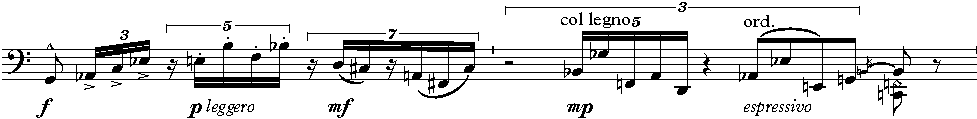
\includegraphics[width=6.5in]{figures/stingray-example.pdf}
        \caption[Self-derivation in Damiani's \emph{Variations for Violoncello}.]{Self-derivation in Damiani's \emph{Variations for Violoncello}.}
        \label{fig:stingray}
    \end{figure}
\end{example}

%--------------------------------------------------------------------------
The framework provided by \cite{Starr1984} is expanded in \cite{Kowalski1987a}, a paper that focuses mostly on the problem of self-derivation. In particular, this focus is restricted to combination matrices with problem sizes two and three, as larger problem sizes are deemed increasingly straightforward to achieve. The technique of folding, as illustrated in Ex.~\ref{self-folded}, is discussed in depth and presented as an alternative to achieving larger than $2 \times 24$ combination matrices \cite[298]{Kowalski1987a}. The direction taken in \cite{Kowalski1987a} differs substantially from \cite{Starr1984} not only in the sense that the former does not stress derivation in general, but also because it constantly emphasizes qualitative aspects of self-derivation. Arguably the greatest contribution in that regard is the introduction of the concept of \emph{merge index} in combination matrices of self-derivation. The merge index measures how row segments are interweaved in a combination matrix and is defined as the number of discrete row segments present in all derived rows, divided by the total number of rows. Ex.~\ref{ex:merge-index} illustrates the basic idea. In general, the more trivial the self-derivation, the lower the merge index \cite[310]{Kowalski1987a}.

%--------------------------------------------------------------------------
\begin{example}
	\cite[314]{Kowalski1987a}
	\label{ex:merge-index}
    The $3 \times 36$ combination matrix $A$ has 10 discrete row segments in all its derived rows. Since there are three derived rows in total, the merge index of $A$ is $10 / 3 = 3.33$. This is considered a rather low merge index.
    \pagebreak
    \begin{equation*}
        A = \left[
        \begin{array}{cccccccccccc|ccccc}
        &&&&&&&&&& 2 & 3 &&&&& \\
        0 & 1 & 4 &&& 10 & 9 & 6 & 5 &&&& 7 & 8 & 11 & 2 & 3 \\
        &&& 7 & 8 &&&&& 11 &&&&&&&
        \end{array}
        \right. \quad \cdots
    \end{equation*}
    \begin{equation}
        \cdots \left. \quad
        \begin{array}{ccccccc|cccccccccccc}
        &&&& 6 & 9 & 10 &&&&&& 0 & 11 & 8 & 7 & 1 & 4 & 5 \\
        &&&&&&&&&&&&&&&&&& \\
        5 & 4 & 1 & 0 &&&& 2 & 3 & 6 & 9 & 10 &&&&&&&
        \end{array}
        \right] \enspace.
    \end{equation}
\end{example}

%--------------------------------------------------------------------------
In a complementary but diametrically opposite approach to \cite{Starr1984}, \cite{Kowalski1987b} proposes an algorithmic view of the specific problem of computing combination matrices of self-derivation. The point of departure of the proposed algorithm is to find the embeddings of transformed row segments in the row itself. These embeddings are pre-computed and stored in a lookup table, then used to construct the first column of a combination matrix by splitting the row into an arbitrary number of initial segments of itself under some transformation \cite[29]{Kowalski1987b}. The algorithm artificially constrains the first column of the combination matrix by disallowing empty cells. This constraint is justified by an increase in performance \cite[30]{Kowalski1987b}. After constructing the first column, the algorithm enumerates all integer partitions of the row size with length equal to the problem size $N$, and finds the next partition that can be used in the next column. In the process, all partitions that cannot be matched with the partitions already present in the previous columns are skipped. Whenever a partition is capable of producing an aggregate, the algorithm moves onto the next column. If all columns up to $N - 1$ are well-formed, the $N$-\textsuperscript{th} column does not need to be verified \cite[31]{Kowalski1987b}. At each column after the first, an order matrix is generated for the column and compared to other transforms in the row class using the $\lor$ operator, as these are binary matrices. If a transform can be found that contains no contradictions with the order matrix for the column at hand, then that transform can be derived from the column. After forming all columns, the algorithm is backtracked so that other possible row transforms may be found. During this phase, if all possibilities were searched, or if some column is incapable of producing a result, then the algorithm resumes the partition enumeration process, trying all possible order matrices for each partition that fits. After trying all partitions for the $(N - 1)$-\textsuperscript{th} column, the algorithm backtracks to the previous column, trying all remaining partitions. After trying all partitions for the second column, a new first column is generated, using the lookup table of embeddings. After trying all combinations of size $N$ from the lookup table of embeddings, the process is repeated reading the embeddings table backwards while attempting to form the first columns, that is, trying to derive retrograde transforms in them, provided the row is not retrograde-invariant. This entire process is repeated with increasing problem sizes, up to the maximum desired size \cite[32]{Kowalski1987b}.

%--------------------------------------------------------------------------
Alg.~\ref{alg:kowalski} shows in pseudocode the entire algorithm described in \cite{Kowalski1987b}. In addition to the procedure illustrated above, the full algorithm iterates over every 12-tone row class, looking for combination matrices of self-derivation in all of them. These row classes are generated in ascending order, as if each row were a 12-digit integer. After generating a new row, if any transform of the row starting with zero is smaller than the row being considered, then this row is skipped. Moreover, the algorithm only considers rows that start with zero, since any other would belong to a row class that has a representative that starts with zero. Rows with a beginning interval $i$ larger than six are also skipped, since those may be considered the inversion of a row beginning with the complement of $i$ \cite[34]{Kowalski1987b}. Similarly, if $i = 5$, then the row may be construed as the $M$ transform of a row in which the first interval is $M(i) = 1$. Rows that have an initial segment of form $\{0, 6, x\}$, with $x > 6$ may also be immediately skipped, since they can be seen as the inverse of a row whose initial segment is $\{0, 6, 12 - x\}$. Analogously, rows that have an initial segment of form $\{0, 6, 5\}$ may also be seen as the $M$ transform of a row whose initial segment is $\{0, 6, 1\}$. Altogether, this reasoning affords contemplating only rows with initial segment in the set $\mathcal{S}$ below \cite[35]{Kowalski1987b}.

%--------------------------------------------------------------------------
\begin{algorithm2e}
\caption{\cite[35, 36, 37]{Kowalski1987b}}
\label{alg:kowalski}
\DontPrintSemicolon
\SetKw{KwGoTo}{goto}
Let $ROW$ be the chromatic scale\;
Find the next permutation of 12 pitch-classes\;
\If{All permutations have been found}{\Return}
Compare $ROW$ with all transforms in its row class that begin with zero\;
\If{Any transform of $ROW$ is numerically lower than $ROW$}{\KwGoTo line 2}
Let $N$ be the smallest problem size minus one\;
Let $IMBED$ be the table of all embeddings of the row class of $ROW$ in itself\;
Let $MAXLEN$ be the longest embedding in the table $IMBED$\;
$N \gets N + 1$\;
\If{$N$ is greater than the largest problem size}{\KwGoTo line 2}
\If{$MAXLEN < 12 / N$}{\KwGoTo line 11}
Take the next $N$-entry combination from the $IMBED$ table\;
\If{All possibilities in $IMBED$ have been tried}{\KwGoTo line 11}
Take the next element of the combination\;
\If{All elements have been tried}{\KwGoTo line 16}
\If{The element duplicates pitch-classes from elements in the same column}{Reduce the element to eliminate duplicates}
\If{The first pitch-class of the element is a duplicate}{\KwGoTo line 16}
\uIf{The columnar aggregate is not complete}{\KwGoTo line 19}
\ElseIf{The columnar aggregate contains fewer than $N$ row segments}{\KwGoTo line 19}
Let $M \gets 1$\;
$M \gets M + 1$\;
\If{$M > N - 1$}{\KwGoTo line 11}
\uIf{All partitions have not been tried for column $M$}{\KwGoTo line 42}
\Else{$M \gets M - 1$}
\uIf{$M > 1$}{\KwGoTo line 34}
\end{algorithm2e}

%--------------------------------------------------------------------------
\setlength{\interspacetitleruled}{0pt}%
\setlength{\algotitleheightrule}{0pt}%

\begin{algorithm2e}
\SetKw{KwGoTo}{goto}
\DontPrintSemicolon
\setcounter{AlgoLine}{39}
\Else{\KwGoTo line 11}
Take the next partition for the current column $M$\;
\If{Partition does not fit $M$}{\KwGoTo line 34}
\If{No aggregates are possible for the partition}{\KwGoTo line 34}
\If{$M < N - 1$}{\KwGoTo line 31}
Let $J \gets 1$\;
$J \gets J + 1$\;
Let $OM$ be the order matrix for column $J$\;
\uIf{$OM$ has not been compared to all order matrices in the row class of $ROW$}{\KwGoTo line 62}
\uElseIf{Column $J$ produced no derivations}{\KwGoTo line 30}
\Else{$J \gets J - 1$}
\uIf{$J = 0$}{\KwGoTo line 73}
\Else{\KwGoTo line 51}
Compare $OM$ with the next transform of $ROW$ using the $\lor$ operator\;
\If{Any contradictions are found}{\KwGoTo line 52}
\uIf{$J = N$ and this is the first derivation of column $J$}{Print the combination matrix}
\Else{Store this derivation}
\uIf{Not all columns have produced a derivation}{\KwGoTo line 50}
\Else{\KwGoTo line 52}
Print all stored alternatives for this combination matrix and \KwGoTo line 30\;
\uIf{$ROW$ is retrograde-invariant}{Go to line 2}
\Else{Take the retrograde of $ROW$}
Change $IMBED$ to point at $R$-embeddings and \KwGoTo line 16\;
\end{algorithm2e}

%--------------------------------------------------------------------------
\begin{equation}
	\label{eq:initial-segment}
	\mathcal{S} = \{\{0, 1\}, \{0, 2\}, \{0, 3\}, \{0, 4\}, \{0, 6, 1\}, \{0, 6, 2\}, \{0, 6, 3\}, \{0, 6, 4\}\} \enspace.
\end{equation}

%--------------------------------------------------------------------------
\noindent The actual implementation of the algorithm comprises a number of enhancements to make it more suitable for certain compositional purposes. Among these enhancements is the inclusion of a device to keep track of the intervallic contents of the row at hand. If a row has too many repeated intervals, it is skipped or rejected \cite[37]{Kowalski1987b}. Other enhancements include limiting the minimum number of intervals and interval classes present in a row, limiting the minimum and maximum acceptable problem sizes, limiting the maximum size of any row segment, limiting the maximum number of empty segments, as well as disallowing $M$ transforms. In addition, the implementation of the algorithm contains a function that returns the merge index for an entire combination matrix \cite[38]{Kowalski1987b}.

%The programming language of choice was FORTRAN, and the implementation does not rely on recursion \cite[40]{Kowalski1987b}. The algorithm was implemented on an IBM 3081 \cite[42]{Kowalski1987b}

%--------------------------------------------------------------------------
Derivation is often approached from the more general context of multiple order functions, which include not only the derivation techniques described above, but also row segments that can belong to more than one dimension of the musical discourse at a time. Mallalieu rows, discussed in Appendix \ref{app:mallalieu}, are a prototypical example. Multiple order functions and Mallalieu rows were extensively studied by Batstone, Morris and Mead \cite{Batstone1972a, Batstone1972b, Morris1977, Mead1988, Mead1989}, and are often a feature of the row itself that does not necessarily extend to combination matrices. In some circumstances, however, they can be used to compose a row that produces high merge indices. In addition, the \emph{partition scheme}, which is the specific merging pattern of segments within a row \cite[245]{Morris1977}, can be explicitly controlled, as illustrated in Ex.~\ref{ex:mof}.

%--------------------------------------------------------------------------
\begin{example}
	\cite[241, 247]{Morris1977}
	\label{ex:mof}
	Constructing a multiple order function row may be accomplished mechanically by devising a partition scheme, aligning the scheme with the order number row, and extracting permutation cycles. These cycles are then matched with the cycles of some $RT_nI$ operation. Consider the partition scheme given by Eq.~\ref{eq:mof}.
	\pagebreak
	\begin{equation}
		\label{eq:mof}
		\left[
        \begin{array}{cccccccccccc}
            0  & 1 & 2  & 3 & 4 & 5 & 6 & 7 & 8 & 9 & 10 & 11 \\
            \hline
               & 0 &    & 1 & 2 &   &   & 3 &   & 4 &    & 5  \\
            11 &   & 10 &   &   & 9 & 8 &   & 7 &   & 6  &
        \end{array}
        \right] \enspace.
	\end{equation}
	\noindent In particular, the lower row of the partition scheme is retrograded in regard to the upper row, which is an important aspect in this type of construction. Extracting permutation cycles from Eq.~\ref{eq:mof} results in the permutation $P = (0 \; 11 \; 5 \; 9 \; 4 \; 2 \; 10 \; 6 \; 8 \; 7 \; 3 \; 1)$. The permutation $P$ can be matched against $T_7 = (0 \; 7 \; 2 \; 9 \; 4 \; 11 \; 6 \; 1 \; 8 \; 3 \; 10 \; 5)$, for example, to construct a series, since both $P$ and $T_7$ have a single cycle of length 12. The series obtained is $S = \{0, 5, 11, 10, 4, 2, 1, 3, 8, 9, 6, 7\}$. This construction yields the following $2 \times 24$ combination matrix of self derivation, where the columns are are $[T_7(S) \; | \; RT_7(S)]$:
	\begin{equation}
		\left[
        \begin{array}{cccccccccccc|cccccccccccc}
        & 0 && 5 & 11 &&& 10 && 4 && 2 && 1 && 3 && 8 & 9 &&& 6 && 7 \\
        7 && 6 &&& 9 & 8 && 3 && 1 && 2 && 4 && 10 &&& 11 & 5 && 0 &
        \end{array}
        \right] \enspace.
	\end{equation}
\end{example}

%--------------------------------------------------------------------------
\section{Objectives and Limitations}

%--------------------------------------------------------------------------
The main objective of this dissertation is to understand the construction of self-deriving combination matrices from an algorithmic standpoint. The techniques proposed in \cite{Starr1984} for self-derivation depart from row segments, aggregate realizations, or columnar aggregates to construct a total order, but the row as a whole is not known before hand. The algorithm proposed in the next chapter will approach the problem of self-derivation from previous knowledge of the row, similarly to the strategy in \cite{Kowalski1987b}. In other words, given a row and a combination matrix size, what are all the possible combination matrices of self-derivation that can be constructed. A fundamental aspect of this algorithm is that it is conceived in all generality, that is, there are no restrictions to row or to problem sizes, hence it will be possible to compute combination matrices for arbitrary $n$-tone equal temperament systems, if the intention is to use the results to organize pitch-classes. However, this generality also implies that self-derivation be used for musical dimensions other than pitch, for which the 12-TET paradigm might not apply. Another important concern is the reduction of the body of solutions into representatives of equivalence classes. Reducing solutions is fundamental for improving execution time and space requirements. The last chapter of the present work will present musical applications of self-derivation as obtained by the proposed model and algorithm. The main relevance of this research is that it extends the field of self-derivation with a novel algorithm based on semi-magic squares. This procedure is simple enough to compute solutions by hand, and powerful enough to compute thousands of solutions in a few milliseconds using a computer. It is also completely general with regard to row and matrix sizes, and allows the composer to use a pre-existing row as input, instead of having the row composed as a byproduct of the procedure. An important contribution is the understanding of how the group $RT_nI$ acts on the set of solutions produced by the algorithm, inducing orbits of different sizes depending on whether the input row is retrograde-invariant or not.

%--------------------------------------------------------------------------
\enlargethispage{\baselineskip}
Despite the many unique contributions, there are certain areas within the field of self-derivation that will not be studied in the present work. In particular, folded and skewed combination matrices are not computed by the algorithm. Folding as described in Ex.~\ref{self-folded} can be construed as an equivalence relation in the sense that combination matrices of different sizes may form an orbit of contractions and expansions. Understanding how solutions of different sizes relate is a fascinating subject for further research, but unfortunately not discussed here. Another important limitation is the fact that only the action of $RT_nI$ is studied, hence multiplication and the cyclic rotation operator are not considered. The former operation is simpler than the latter if the present algorithm were to be improved. However, the latter is arguably more relevant. Eq.~\ref{eq:scotto-folded} presents an important example of how cyclic rotation may appear when folding combination matrices of self-derivation. Multiplication, on the other hand, is controversial for not preserving intervallic content. Magic squares in themselves have amazing compositional applications, which can be found in the music of John Cage, Peter Maxwell Davies and Zack Browning. This dissertation will discuss semi-magic squares only in conjunction with self-derivation. Even within the realm of self-derivation, however, semi-magic squares present a potential for musical syntax, as one can go from one square to another via matrix operations. This potential is nevertheless left for future research. Multiple order functions, including Mallalieu rows, are well-understood. Mallalieu rows, in particular, do not necessarily yield combination matrices of self-derivation with a high merge index. In general, multiple order functions are useful for composing rows, but their relevance to combination matrices is limited when cyclic rotation is not allowed. Therefore, self-derivation shall not be addressed here from the perspective of multiple order functions. Having an efficient algorithm to compute self-deriving matrices is an important component in the algorithmic composition of electroacoustic music. Devising algorithms for both real-time and non-real-time generation of electroacoustic music, where self-derivation is applied to arbitrary parameters of a musical composition, is also not discussed in this paper, but represents a fundamental direction for future research.

%--------------------------------------------------------------------------
\enlargethispage{\baselineskip}
The ideas presented throughout the theoretical framework in the next chapter assume a wealth of prior knowledge. A set-theoretic view of 20\textsuperscript{th}-century musical analysis, as taught in graduate-level courses, that is, familiarity with such basic concepts as contour, pitch, and pitch-class spaces, intervals and interval classes, set and row classes, twelve-tone operations, and associated group-theoretic notions is assumed. Likewise, solid knowledge of 12-tone theory, including the hexachordal combinatoriality seen in the works of Schoenberg, and the trichordal combinatoriality seen in the works of Babbitt, as well as the methods that afford constructing such combinatorialities will not be discussed, but assumed. Also necessary is a working knowledge of abstract and linear algebra, to the extent that many graduate texts in atonal music theory will require. Preliminary results on the topic of group actions are included in Appendix \ref{app:group-actions}. C and C++ programming, and basic concepts of computer science are not included, and only a very superficial knowledge of computer science is necessary to understand the theoretical framework. More involved correctness proofs and complexity analyses of the algorithms presented in the next chapter will be omitted in order to maintain the focus on the musical relevance of such constructs.

%--------------------------------------------------------------------------
\chapter{THEORETICAL FRAMEWORK}

%TODO: This problem is NP-hard and is a satisfiability problem similar to Sudoku and the 8-Queens.

%--------------------------------------------------------------------------
\section{Defining an algorithm to compute a row class}

%--------------------------------------------------------------------------
In a traditional setting, a composer will usually define a class of transforms of a basic row by computing by hand what is commonly denoted a 12-tone matrix. The general procedure usually consists of filling the top row of the matrix with a transform of the 12-tone row beginning with zero. The second step is to fill the leftmost column of the matrix with the inverse transform of the top row. The subsequent steps comprise going row-by-row, filling them with a transposition of the top row. The particular transposition for each 12-tone row is given by the first element of the matrix row at hand, which in turn corresponds to an element in the leftmost column. The 12-tone matrix will hold all 48 transforms of a row: reading every row from left to right gives all transpositions, reading them from right to left gives all retrogrades, reading all columns from top to bottom gives all inversions, and reading them from bottom to top gives all retrograde inversions. Although somewhat tedious, computing 12-tone matrices by hand is a well-established procedure. The 48 transforms that can be inferred from the matrix are not necessarily unique, given that a 12-tone may be retrograde, or retrograde-inverse invariant. It is straightforward to generalize the procedure to $n$-tone matrices. However, the graphical idea of reading the matrix from right to left, or bottom to top, is not ideal for computing self-deriving combination matrices, as it is faster to read a transform of a row that is written contiguously in memory. Another caveat is that the procedure does not necessarily define a canonical form for the top row. Every row in a matrix is a representative of an equivalence class of rows under the action of $RT_nI \cong D_{24} \oplus \mathbb{F}_2$ \cite[127]{FripertingerLackner2015}. The size of each orbit is $4n$ if the row is not retrograde or retrograde-inverse invariant, and $2n$ otherwise. Defining a canonical form for the first row in a data structure that holds a row class is desirable in any algorithm that iterates through row classes in lexicographic order.

%--------------------------------------------------------------------------
Listing~\ref{getCanonicalForm} describes an algorithm that produces a canonical form for a row. The canonical form defined in this implementation is simply the least element in a lexicographic ordering of a row class. Given an arbitrary representative of a row class, that representative will be considered retrograded if any interval class between two consecutive elements of the row, counted from right to left, is strictly less than the corresponding interval class counted from left to right. Most procedures described in this chapter and the next rely on aliases for certain primitive data types, which are given Listing~\ref{typedefs}.

%--------------------------------------------------------------------------
\begin{lstlisting}[caption={Defining aliases for common primitive data types.},label={typedefs}]
typedef signed char number;
typedef unsigned short range;
typedef unsigned long length;
\end{lstlisting}

%TODO: explain how these primitives were chosen

%--------------------------------------------------------------------------
Finding the interval class between two pitch-classes is illustrated in Listing~\ref{intervalClass}, which takes as input two pitch-classes $a$ and $b$, and the base $n$, returning the interval class between the two. The interval class between $a \pmod n$ and $b \pmod n$ is expressed mathematically as $\min\{(a - b) \pmod n, (b - a) \pmod n\}$.

%--------------------------------------------------------------------------
\begin{lstlisting}[caption={Computing the interval class between two pitch-classes.},label={intervalClass}]
number intervalClass(number a, number b, number rowSize) {
    number interval = abs(a - b);
    return min(interval, rowSize - interval);
}
\end{lstlisting}

%--------------------------------------------------------------------------
\begin{enumerate}
\item Listing~\ref{intervalClass} takes as input two pitch-classes $a$ and $b$, as well as a base $n$ such that $a, b \in \mathbb{Z} / n \mathbb{Z}$.
\item Line 2 simply computes the distance between $a$ and $b$.
\item Line 3 returns the least between the interval computed in line 2 and its complement, that is, the interval class between the two given pitch-classes.
\end{enumerate}

%--------------------------------------------------------------------------
The procedure for determining whether a row is retrograded utilizes Listing~\ref{intervalClass} as a subroutine and is outlined in Listing~\ref{isRetrograded}. The first parameter taken by Listing~\ref{isRetrograded} is the row at hand, which can be any representative of its row class.

%--------------------------------------------------------------------------
\begin{lstlisting}[caption={Determining whether a representative of a row class is retrograded.},label={isRetrograded}]
bool isRetrograded(const number *row, number rowSize, bool isInvariant) {
    if (isInvariant || rowSize < 5)
        return false;

    number front, back;

    for (number i = 0; i < rowSize / 2; ++i) {
        front = intervalClass(row[i + 1], row[i], rowSize);
        back = intervalClass(row[rowSize - i - 1], row[rowSize - i - 2], rowSize);

        if (back < front)
            return true;
    }

    return false;
}
\end{lstlisting}

%--------------------------------------------------------------------------
\begin{enumerate}
\item Listing~\ref{isRetrograded} has three parameters, namely a pointer to a row, its size, and a boolean representing whether the row is retrograde or retrograde inverse-invariant. The returned value is another boolean indicating whether the row is retrograded or not.
\item Lines 2 and 3 perform a sanity check. It is straightforward to see that all rows of size 4 or less are necessarily retrograde or retrograde inverse-invariant. If, on the other hand, a row with 5 or more elements is known to be invariant, the test is also skipped.
\addtocounter{enumi}{2}
\item Line 5 declares the variables that will represent the row's interval classes seen from left to right, and from right to left, respectively.
\addtocounter{enumi}{2}
\item Lines 8 and 9 simply update the variables \emph{front} and \emph{back} using Listing~\ref{intervalClass} defined above. As $i$ increases, \emph{front} traverses half of the interval classes in the row from left to right, whereas \emph{back} does the same from right to left, that is, \emph{back} looks at the row as if it were retrograded.
\addtocounter{enumi}{2}
\item Line 11 compares the front and back interval classes and line 12 returns true if any interval class seen from right to left is strictly less than the corresponding interval class seen from left to right, which would indicate that retrograding the row would produce a row with a lower lexicographic position than the one given as input.
\addtocounter{enumi}{3}
\item If all interval classes seen from both directions are equal, then the row is retrograde or retrograde inverse-invariant. Line 15 then returns false to avoid unnecessarily reversing a row that is invariant.
\end{enumerate}

%--------------------------------------------------------------------------
The next step in determining the canonical form of a row consists of finding whether its inverse has a lower lexicographic position within the row class. The procedure is described in Listing~\ref{isInverted}, which in turn depends on two small subroutines, namely Listing~\ref{modulo} and Listing~\ref{isOwnInverse}. The former simply computes $modulo(x, n) = x \pmod{n}$. However, it needs to be defined as a subroutine this way because the result of the C-language built-in modulo operator is signed, and for practical reasons that will be elaborated in the next sections, it is best that all pitch-classes be represented as unsigned integers ranging from $0$ to $n - 1$.

%--------------------------------------------------------------------------
\begin{lstlisting}[caption={A subroutine to compute $x \pmod{n}$ such that the result is non-negative.},label={modulo}]
number modulo(number x, number base) {
    x %= base;
    return x < 0 ? x + base : x;
}
\end{lstlisting}

%--------------------------------------------------------------------------
\begin{enumerate}
\item The inputs to Listing~\ref{modulo} are a number $x$ and a base $n$.
\item Line 2 simply computes $x \pmod{n}$ using the C-language built-in modulo operator.
\item Line 3 then returns the congruence class in the range $[0, n - 1]$.
\end{enumerate}

%--------------------------------------------------------------------------
Listing~\ref{isOwnInverse} is a simple convenience method that is used to check whether $x \equiv x \pmod{n}$, which is also needed in Listing~\ref{isInverted}.

%--------------------------------------------------------------------------
\begin{lstlisting}[caption={A subroutine that returns true if a pitch-class is its own inverse.},label={isOwnInverse}]
bool isOwnInverse(number x, number base) {
    return x == 0 || x == base - x;
}
\end{lstlisting}

%--------------------------------------------------------------------------
\begin{enumerate}
\item The input $x$ is assumed to be in the range $[0, n - 1]$.
\item Since $x$ is non-negative, it can only be its own inverse if it is the identity, or if $x \equiv -x \pmod{n}$. It is also possible to check that if $n$ is even and $x$ is equal to $n / 2$, then $x$ is its own inverse. But this alternative method is more expensive that the computation performed in line 2.
\end{enumerate}

%--------------------------------------------------------------------------
In order to determine whether the inverse transform of a row has a lower lexicographic position than itself, it is necessary in this implementation to consider if its retrograde transform also sits in a lower lexicographic position. Therefore a call to Listing~\ref{isInverted} requires a previous call to Listing~\ref{isRetrograded}, since the result of the latter is used as the last argument passed to Listing~\ref{isInverted}.

%--------------------------------------------------------------------------
\begin{lstlisting}[caption={Determining whether a representative of a row class is inverted.},label={isInverted}]
bool isInverted(const number *r, number rowSize, bool R) {
    if (R) {
        for (number i = rowSize - 1; i >= rowSize / 2; --i) {
            number mod = modulo(r[i] - r[rowSize - 1], rowSize);

            if (!isOwnInverse(mod, rowSize))
                return mod > rowSize - mod;
        }
    } else {
        for (number i = 0; i < rowSize / 2; ++i) {
            number mod = modulo(r[i] - r[0], rowSize);

            if (!isOwnInverse(mod, rowSize))
                return mod > rowSize - mod;
        }
    }

    return false;
}
\end{lstlisting}

%--------------------------------------------------------------------------
\begin{enumerate}
\item The inputs are a row, its size, and a boolean representing whether the row is retrograded.
\addtocounter{enumi}{1}
\item If $r$ is retrograded, line 3 begins iteration in reverse order, that is, starting with the last element of the row.
\item Line 4 computes the ordered interval between the pitch-class at hand, and the first pitch-class of the row, which in this case is the last because the row is retrograded.
\addtocounter{enumi}{1}
\item Line 6 checks if the interval is not its own inverse and, if not, line 7 checks if the interval is greater than its inverse. If so, an inverted form of the row would sit in a lower lexicographic position within the entire row class, and the row is inverted.
\addtocounter{enumi}{3}
\item If the input row is not retrograded, then lines 10 to 14 perform essentially the same check as the previous branch, only traversing the row from left to right, instead of the right to left traversal done for a retrograded row. In both branches, it is important to note that the loops iterate at most twice. If the row size is odd, then the very first iteration will decide if the row is inverted. If, on the other hand, the row size is even, then there is the possibility that the very first interval will be its own inverse, in which case the next iteration will invariably be able to tell if the row is inverted.
\addtocounter{enumi}{7}
\item Line 18 should never be reached for well-defined inputs, and is included for correctness.
\end{enumerate}

%--------------------------------------------------------------------------
Determining that an arbitrary representative of a row class is retrograded or inverted are essential subroutines used in Listing~\ref{getCanonicalForm}, which in turn does transform the input row into its canonical form. This transformation happens in Listing~\ref{getTransformInPlace}, and the latter relies on a straightforward method to swap row entries in place, which is described below in Listing~\ref{swapInPlace}.

%--------------------------------------------------------------------------
\begin{lstlisting}[caption={Swapping two entries in a row.},label={swapInPlace}]
void swapInPlace(number *row, number i, number j) {
    number tmp = row[i];
    row[i] = row[j];
    row[j] = tmp;
}
\end{lstlisting}

%--------------------------------------------------------------------------
The procedure in Listing~\ref{swapInPlace} is very common-place, so the details are omitted. Listing~\ref{getTransformInPlace} is also straightforward and represents the main subroutine in Listing~\ref{getCanonicalForm}.

%--------------------------------------------------------------------------
\begin{lstlisting}[caption={Transforming a row in place.},label={getTransformInPlace}]
void getTransformInPlace(number *row, number rowSize, number T, bool I, bool R) {
    if (R) {
        for (number i = 0; i < rowSize / 2; ++i)
            swapInPlace(row, i, rowSize - 1 - i);
    }

    if (I) {
        for (number i = 0; i < rowSize; ++i)
            row[i] = (rowSize - row[i] + T) % rowSize;
    } else if (T != 0 % rowSize) {
        for (number i = 0; i < rowSize; ++i)
            row[i] = (row[i] + T) % rowSize;
    }
}
\end{lstlisting}

%--------------------------------------------------------------------------
\begin{enumerate}
\item The inputs are a row, its size, a non-negative integer representing an offset to be added to the entire row, a boolean representing whether the row is inverted, and another boolean representing whether the row is retrograded.
\addtocounter{enumi}{1}
\item If the row is retrograded, lines 3 and 4 simply reverse the row using Listing~\ref{swapInPlace}.
\addtocounter{enumi}{4}
\item If the row is inverted, lines 8 and 9 invert the row and add the offset to each row entry.
\addtocounter{enumi}{2}
\item Otherwise, if the row is not inverted, lines 11 and 12 only add the offset to the entire row.
\end{enumerate}

%--------------------------------------------------------------------------
The procedure illustrated in Listing~\ref{getTransformInPlace} is used below in Listing~\ref{getCanonicalForm}, but it will also be used many times over to construct a row class in memory. In the particular case where the canonical form of the row is desired, that is, the lowest element in a lexicographic ordering of the row class, the offset used will be the additive inverse of the row's first element. It is important to observe that Listing~\ref{getCanonicalForm} requires prior knowledge as to whether the row is retrograde or retrograde inverse-invariant. In the grand scheme of things, that knowledge will already be available when calling Listing~\ref{getCanonicalForm}.

%--------------------------------------------------------------------------
\begin{lstlisting}[caption={Transforming a row into its canonical form.},label={getCanonicalForm}]
void getCanonicalForm(number *row, number rowSize, bool isInvariant) {
    bool R = isRetrograded(row, rowSize, isInvariant);
    bool I = isInverted(row, rowSize, R);
    number T = row[R ? rowSize - 1 : 0];
    getTransformInPlace(row, rowSize, I ? T : rowSize - T, I, R);
}
\end{lstlisting}

%--------------------------------------------------------------------------
\begin{enumerate}
\item The inputs are a row, its size, and whether the row is retrograde or retrograde inverse-invariant.
\item Lines 2 and 3 simply call Listing~\ref{isRetrograded} and Listing~\ref{isInverted} respectively, storing the results.
\addtocounter{enumi}{1}
\item Line 4 just stores the first element of the row, which may be the last if the row is retrograded.
\item Line 5 is a call to Listing~\ref{getTransformInPlace}. The third argument is the additive inverse of the row's start element. It varies, naturally, if the row is inverted.
\end{enumerate}

%--------------------------------------------------------------------------
The purpose of the procedure described in Listing~\ref{getRowClass} is to store an entire row class contiguously in memory. That consists of creating an array large enough to hold all transforms of a row, and sequentially copying said transforms into this array. Even for rows whose bases are considered large, a row class under $RTn_I$ is still very small. Thus holding these transforms in memory makes sense for execution speed purposes. The size of the row class array depends on whether the row is reverse or reverse inverse-invariant. The row class array begins with the canonical form of the row, followed by all its transpositions, in ascending order, followed by all transpositions of the inversion of the canonical form, also in ascending order. If the row is not reverse or reverse inverse-invariant, the row class array is appended by all transpositions of the reverse of the canonical order, followed by all transpositions of the retrograde inverse of the canonical order. Therefore, the overall size of the row class array is $2n^2$ if the row is retrograde or retrograde inverse-invariant, or $4n^2$ otherwise, where $n$ is the row size. The main routine for creating the row class array is described in Listing~\ref{getRowClass}. It depends on two subroutines, namely Listing~\ref{isRetrogradeInvariant} and Listing~\ref{isRetrogradeInverseInvariant} that are described below.

%--------------------------------------------------------------------------
\begin{lemma}
	\label{retrograde-invariance}
	In a retrograde-invariant row, the interval between every entry seen from left to right, and the corresponding entry seen from right to left, must equal half the size of the row. In particular, a row with odd size greater than $3$ cannot be retrograde-invariant.
	\begin{proof}
	Regard the row as a sequence of order numbers $\{0, 1, \cdots, n - 1\}$. If $n$ is even, the retrograde operation induces the permutation of order numbers
	\begin{equation}
		P = (0 \; n - 1) \; (1 \; n - 2) \; \cdots \; (\tfrac{n}{2} - 1 \; \tfrac{n}{2}) \enspace .
	\end{equation}
	If $n$ is odd, the retrograde operation induces the permutation of order numbers
	\begin{equation}
		P = (0 \; n - 1) \; (1 \; n - 2) \; \cdots \; (\lfloor \tfrac{n}{2} \rfloor) \enspace .
	\end{equation}
	Since $P$ is a transposition, the only possibility is $P = T_{\frac{n}{2}}$ with $n$ even.
	\end{proof}
\end{lemma}

%--------------------------------------------------------------------------
\begin{lstlisting}[caption={Determining whether a row is retrograde-invariant.},label={isRetrogradeInvariant}]
bool isRetrogradeInvariant(const number *row, number rowSize) {
    if (rowSize > 4 && rowSize % 2 == 1)
        return false;

    number half = rowSize / 2;

    for (number i = 0; i < half; ++i) {
        if (modulo(row[rowSize - i - 1] - row[i], rowSize) != half)
            return false;
    }

    return true;
}
\end{lstlisting}

%--------------------------------------------------------------------------
\begin{enumerate}
\item The only inputs are a row and its size.
\item Line 2 utilizes Lem.~\ref{retrograde-invariance} as a sanity check. If the test in line 2 succeeds, line 3 returns false.
\addtocounter{enumi}{2}
\item Line 5 just computes half the row size for convenience. Retrograde-invariance can be determined by iterating through at most half the size of the row.
\addtocounter{enumi}{1}
\item Line 7 iterates through the row from left to right, and line 8 applies Lem.~\ref{retrograde-invariance}. Line 9 then returns false if any of the intervals is not equal to half the row size.
\addtocounter{enumi}{4}
\item If all pairs coming from both directions are equal to half the row size, then the row is retrograde-invariant and line 12 returns true.
\end{enumerate}

%--------------------------------------------------------------------------
Unlike retrograde invariance, every row size can produce retrograde inverse-invariant rows. A simple example is the row of any size with the lowest lexicographic order. If $n = 12$, this is a chromatic scale. Retrograding, inverting, and transposing by $-1$ always yields back the initial row. Listing~\ref{isRetrogradeInverseInvariant} outlines the procedure in all generality.

%--------------------------------------------------------------------------
\begin{lemma}
	\label{retrograde-inverse-invariance}
	In a retrograde inverse-invariant row $r$, the sum of every entry seen from left to right, and the corresponding entry seen from right to left, must be equal to $x = r_0 + r_{n - 1} \pmod{n}$, where $n$ is the base of the row. In particular, if $n$ is odd, the element at the center of the row plus itself must also be equal to $x$. 
	\begin{proof}
	The index of inversion between two pitch-classes is their sum. To see that, let $a$ and $b$ be pitch-classes. It follows
	\begin{equation}
		a = T_xI(b) \iff a = T_x(-b) \iff a = x - b \iff a + b = x \enspace .
	\label{eq:retrograde-inverse-invariance}
	\end{equation}
	If $x = r_0 + r_{n - 1} \pmod{n}$, then $x$ is the index of inversion between the first and last elements of $r$. Since $r$ is retrograde inverse-invariant, this forces every pair of corresponding elements in $r$ from both directions to have the same index of inversion. If $n$ is odd, the element $c$ at the center must be invariant under $T_xI$, since it is a fixed point under $R$. By Eq.~\ref{eq:retrograde-inverse-invariance}, $c = T_xI(c) \iff c + c = x$, as desired.
	\end{proof}
\end{lemma}

%--------------------------------------------------------------------------
\begin{lstlisting}[caption={Determining whether a row is retrograde inverse-invariant.},label={isRetrogradeInverseInvariant}]
bool isRetrogradeInverseInvariant(const number *row, number rowSize) {
    number half = rowSize / 2;
    number first = modulo(row[rowSize - 1] + row[0], rowSize);

    for (number i = 1; i < half; ++i) {
        if (modulo(row[rowSize - i - 1] + row[i], rowSize) != first)
            return false;
    }

    return true;
}
\end{lstlisting}

%--------------------------------------------------------------------------
\begin{enumerate}
\item The inputs are a row and its size.
\item Line 2 computes half the row size for convenience. Like Listing~\ref{isRetrogradeInvariant}, retrograde inverse invariance can be determined by traversing at most half the row size.
\item Line 3 computes $r_0 + r_{n - 1} \pmod{n}$ for later use.
\addtocounter{enumi}{1}
\item Line 5 begins iteration from the second entry onward, since the first pair was already computed in line 3. Line 6 then compares the subsequent corresponding pairs, and line 7 returns false if any of them is not equal to the first pair.
\addtocounter{enumi}{4}
\item If line 10 is reached, it means the row is retrograde inverse-invariant, so the algorithm returns true.
\end{enumerate}

%--------------------------------------------------------------------------
The procedure to compute and store an entire row class in memory is outlined below in Listing~\ref{getRowClass}. It returns a memory address that must be freed by the caller. While computing combination matrices of self-derivation, this memory location will be held for the duration of the program, and possibly also be shared by many different threads of execution. The procedure makes heavy use of Listing~\ref{getTransformInPlace} to sequentially store in memory all transforms of the canonical form of the row. It also takes the input row and transforms it in-place into its canonical form. Any representative of a row class can therefore be used to construct a row class with Listing~\ref{getRowClass}.

%--------------------------------------------------------------------------
\begin{lstlisting}[caption={Computing and storing a row class in memory.},label={getRowClass}]
number *getRowClass(range *classSize, number *row, number rowSize, bool isInvariant) {
    getCanonicalForm(row, rowSize, isInvariant);
    *classSize = isInvariant ? rowSize * 2 : rowSize * 4;

    number *rowClass = malloc(rowSize * *classSize * sizeof(number));
    memcpy(rowClass, row, rowSize * sizeof(number));

    for (number i = 1; i < rowSize; ++i) {
        number *rep = &rowClass[i * rowSize];
        memcpy(rep, rowClass, rowSize * sizeof(number));
        getTransformInPlace(rep, rowSize, i, false, false);
    }

    for (number i = rowSize; i < rowSize * 2; ++i) {
        number *rep = &rowClass[i * rowSize];
        memcpy(rep, rowClass, rowSize * sizeof(number));
        getTransformInPlace(rep, rowSize, i, true, false);
    }

    if (*classSize == rowSize * 2)
        return rowClass;

    for (number i = rowSize * 2; i < rowSize * 3; ++i) {
        number *rep = &rowClass[i * rowSize];
        memcpy(rep, rowClass, rowSize * sizeof(number));
        getTransformInPlace(rep, rowSize, i, false, true);
    }

    for (number i = rowSize * 3; i < rowSize * 4; ++i) {
        number *rep = &rowClass[i * rowSize];
        memcpy(rep, rowClass, rowSize * sizeof(number));
        getTransformInPlace(rep, rowSize, i, true, true);
    }

    return rowClass;
}
\end{lstlisting}

%--------------------------------------------------------------------------
\begin{enumerate}
\item The inputs are a pointer to the size of the row class, which will be computed by Listing~\ref{getRowClass} and stored in the address provided, a row, its size, and a boolean representing whether the row is retrograde or retrograde inverse-invariant. This boolean will be computed by the caller before calling Listing~\ref{getRowClass}, utilizing the procedures described in Listing~\ref{isRetrogradeInvariant} and Listing~\ref{isRetrogradeInverseInvariant}. The output is a memory location containing the entire row class.
\item As mentioned above, line 2 simply computes the canonical form of the given row in place.
\item Line 3 computes the class size based on whether the row is retrograde or retrograde inverse-invariant. It is important to notice here that the row class size is not the length of the row class array, but the number of transforms of the canonical form that the row class array contains. This number is stored in the address provided by the caller.
\addtocounter{enumi}{1}
\item Line 5 allocates in the heap the memory space that will be used to store the entire row class, and line 6 copies the canonical form of the row to the beginning of this allocated space.
\addtocounter{enumi}{2}
\item Line 8 starts from the second row in the row class, which is the first transposition of the canonical form, and the block adds all subsequent transpositions to the row class. Line 9 computes the address where the current transposition should start, line 10 copies the canonical form of the row into this address, and line 11 transforms the canonical form into the desired transposition in place. 
\addtocounter{enumi}{5}
\item Line 14 starts from the $n$\textsuperscript{th} row in the row class, that is, the $T_0I$ transform of the row. Lines 15 to 17 add the subsequent $T_nI$ transforms of the canonical form of the row in the same way the $T_n$ transforms were added above, only specifying in the call to Listing~\ref{getTransformInPlace} that the transforms now need to be inverted.
\addtocounter{enumi}{5}
\item Line 20 checks if the row is retrograde or retrograde inverse-invariant and, if so, halts the process and returns the memory location allocated in line 5.
\addtocounter{enumi}{2}
\item If the row is is retrograde or retrograde inverse-invariant, lines 23 to 26 add all $RT_n$ transforms of the row to the row class as above.
\addtocounter{enumi}{5}
\item Similarly, lines 29 to 32 add all the $RT_nI$ transforms of the row.
\addtocounter{enumi}{5}
\item Line 36 then simply returns the memory location allocated in line 5.
\end{enumerate}

%--------------------------------------------------------------------------
\section{Defining an algorithm to compute semi-magic squares}

A key component in the definition of a combination matrix of self-derivation is a semi-magic square. By definition, a semi-magic square is a square matrix where the sum of all elements, for each row and column, is a constant. For our purposes, that constant will be the base $n$ of the row. Seeing each entry in a semi-magic square as a real number and dividing each entry in the matrix by $n$ produces a doubly stochastic matrix, in which every row and every column sum to one. A magic square is a semi-magic square where, in addition, both main diagonals add up to the same constant as the rows and columns. By the definition above of a semi-magic square, every row therein is a permutation of an integer partition of $n$. In fact, every column is also a permutation of an integer partition of $n$, but the algorithm described below in Listing~\ref{allPartitionsRecursive} shall concentrate on computing all integer partitions of $n$ and their permutations as rows that will ultimately become the rows of a semi-magic square. Since these integer partitions of $n$ are completely independent of the row at hand, they can be computed only once for each $n$ and stored as a file, speeding up the process of computing combination matrices for other rows. Before describing Listing~\ref{allPartitionsRecursive}, a couple subroutines for reading and writing files are outlined.

%--------------------------------------------------------------------------
\begin{lstlisting}[caption={Retrieving the size of a file.},label={getFileSize}]
long getFileSize(FILE *file) {
    fseek(file, 0, SEEK_END);
    long fileSize = ftell(file);
    fseek(file, 0, SEEK_SET);
    return fileSize;
}
\end{lstlisting}

Listing~\ref{getFileSize} is a completely common-place procedure in the C-language, and its details are omitted. It is used as a subroutine in Listing~\ref{readFile}, which is described next.

%--------------------------------------------------------------------------
\begin{lstlisting}[caption={Reading the contents of a file.},label={readFile}]
number *readFile(const char *fileName, length *numLines, number problemSize) {
    FILE *file = fopen(fileName, "rb");

    if (file == NULL)
        return NULL;

    long fileSize = getFileSize(file);
    number *buffer = malloc(fileSize);
    *numLines = (length) (fileSize / sizeof(number)) / problemSize;
    fread(buffer, fileSize, 1, file);
    fclose(file);

    return buffer;
}
\end{lstlisting}

\begin{enumerate}
\item The inputs are the file name, assuming both the main executable and the file are in the same folder, a memory address where the number of lines read will be stored, and the problem size, which is the size of the magic square. The output is a memory location with the contents of the file, or a NULL pointer if the operation fails.
\item Line 2 simply opens the file at the given path for reading. Line 4 performs a sanity check and line 5 returns a NULL pointer if the file cannot be read.
\addtocounter{enumi}{4}
\item Line 7 is a call to Listing~\ref{getFileSize} so that the correct amount of memory can be allocated. The value computed in line 7 is already in bytes. Line 8 then allocates the memory whose address will be returned.
\addtocounter{enumi}{1}
\item Line 9 computes the number of lines in the file, that is, the number of integer partitions of $n$ with length \emph{problemSize} that have been previously computed and stored in the file. The value is then stored in the memory address provided in the input list to store the number of lines in the file.
\item Line 10 simply reads the entire contents of the file into the buffer allocated in line 8, line 11 frees the FILE data structure created in line 2, and line 13 returns the allocated memory. It is the responsibility of the caller to free this memory when no longer needed.
\end{enumerate}

The procedure described in Listing~\ref{writeAllPartitions} effectively writes all integer partitions of $n$ with a certain size to a file. It depends on Listing~\ref{allPartitionsRecursive} to compute all said partitions recursively, which is described next. One important feature of Listing~\ref{allPartitionsRecursive} is that it skips partitions whose all but one entries are zero. The reason for this is because the remaining entry would be forced to be equal to $n$. In any semi-magic square where there is an entry equal to $n$, both the row and column to which this entry belongs will necessarily contain only zeros except, of course, for the entry with value $n$. This means that the linearized top of the combination matrix at that semi-magic square's column will inevitably be trivially polyphonized, that is, the corresponding square cell would simply have the entire row at the top. Therefore any combination matrix can be extended by adding a column and a row at an arbitrary indices, and making that square entry contain $n$ elements, that is, a linearized statement of a row form. Since this procedure is completely general, the semi-magic squares computed below include entries only up to $n - 1$.

%--------------------------------------------------------------------------
\begin{lstlisting}[caption={Recursively computing all partitions of a number $n$ and permutations thereof with a certain size.},label={allPartitionsRecursive}]
void allPartitionsRecursive(number *tmp, number currentSize, number problemSize, number currentSum, number rowSize, FILE *file) {
    if (currentSize == problemSize - 1) {
        if (currentSum > 0) { // skip the [0, ..., 0, rowSize] partition
            tmp[currentSize] = rowSize - currentSum;
            fwrite(tmp, sizeof(number), problemSize, file);
        }

        return;
    }

    for (number i = 0; i < rowSize; ++i) {
        if (i + currentSum <= rowSize) {
            tmp[currentSize++] = i;
            allPartitionsRecursive(tmp, currentSize, problemSize, i + currentSum, rowSize, file);
            currentSize--;
        }
    }
}
\end{lstlisting}

\begin{enumerate}
\item The inputs are the address of some scratch memory previously allocated with the same length of the problem size, the current number of entries already placed in the scratch memory, the problem size, the current sum of the entries in the scratch memory, the base $n$, and a pointer to a FILE data structure where the partitions will be stored, line by line.
\item Line 2 deals with the base case of the recursion, that is, when the current number of elements in the scratch memory is one less than the problem size. If that is the case, then the last element in the scratch memory array must be equal to $n$ minus the sum of all previous elements.
\item Line 3 deals with the edge case where all entries up to problem size minus one are zero. That would force the very last element of the scratch memory array to be equal to $n$ which, by the discussion above is avoided in this implementation.
\item Line 4 sets the last element of the scratch memory array to $n$ minus the sum of its previous elements and line 5 writes the current partition to the given file. Having completed an entire partition, line 8 returns, so the function recurses no further.
\addtocounter{enumi}{6}
\item For the recursion cases where the scratch memory array has been filled with less than problem size minus one elements, the loop in line 11 iterates from zero to $n - 1$. Line 12 is a sanity check that the sum of the current element being appended to the scratch memory array with the current sum of all elements so far introduced is no greater than $n$. Line 13 then appends the current element to the end of the scratch memory array, increases the current size counter, and line 14 pushes to the call stack another recursive call to Listing~\ref{allPartitionsRecursive}.
\addtocounter{enumi}{1}
\item Line 15 backtracks the current size so that all combinations of integers in the range $[0, n - 1]$ are tried.
\end{enumerate}

Listing~\ref{writeAllPartitions} described below is essentially a wrapper around Listing~\ref{allPartitionsRecursive}. Partitions files are saved in the same location where the main executable is built, in order to facilitate dealing with file paths. In general, these files are very small even for large $n$, but the speed gains in precomputing them are worthwhile, given the recursive nature of Listing~\ref{allPartitionsRecursive}.

%--------------------------------------------------------------------------
\begin{lstlisting}[caption={Writing all partitions to a file.},label={writeAllPartitions}]
void writeAllPartitions(number problemSize, number rowSize) {
    char fileName[32];
    sprintf(fileName, "all_partitions_%i_%i.dat", problemSize, rowSize);
    FILE *file = fopen(fileName, "wb");

    number *tmp = malloc(problemSize * sizeof(number));
    allPartitionsRecursive(tmp, 0, problemSize, 0, rowSize, file);

    free(tmp);
    fclose(file);
}
\end{lstlisting}

\begin{enumerate}
\item The inputs are a problem size, which is the size of the semi-magic square, and a row size, which is the row base $n$.
\item Line 2 creates an array of 32 characters to hold the file name. This file name array length is large enough to accommodate all file names in this implementation. Line 3 writes the name of the file into the buffer defined in the previous line, and line 4 opens a C-type FILE for writing at the specified path.
\addtocounter{enumi}{3}
\item Line 6 allocates the scratch memory needed for the call to Listing~\ref{allPartitionsRecursive} in the following line. Being that Line 7 is the bottommost call on the call stack for Listing~\ref{allPartitionsRecursive}, the arguments given for the current size and current sum parameters are both zero.
\addtocounter{enumi}{2}
\item Line 9 frees the scratch memory used in the calls to Listing~\ref{allPartitionsRecursive}, and line 10 closes and releases the file created in line 4.
\end{enumerate}

The counterpart to Listing~\ref{writeAllPartitions} is Listing~\ref{readAllPartitions}, which is designed to not only read a partitions file, but to also generate one in case the particularly sought partitions file had not been previously created.

%--------------------------------------------------------------------------
\begin{lstlisting}[caption={Reading all partitions from a file.},label={readAllPartitions}]
number *readAllPartitions(length *numPartitions, number problemSize, number rowSize) {
    char fileName[32];
    sprintf(fileName, "all_partitions_%i_%i.dat", problemSize, rowSize);

    number *allPartitions = readFile(fileName, numPartitions, problemSize);

    if (allPartitions == NULL) {
        printf("Writing partitions file...\n");
        writeAllPartitions(problemSize, rowSize);
        allPartitions = readFile(fileName, numPartitions, problemSize);
    }

    return allPartitions;
}
\end{lstlisting}

\begin{enumerate}
\item The inputs are a memory address to store the number of lines in the partitions file to be read, the problem size and the row size. The output is a memory address with the contents of the partitions file. It is the responsibility of the caller to free the returned memory when no longer needed.
\item Lines 2 and 3 store the file name in a buffer, similarly to Listing~\ref{writeAllPartitions}.
\addtocounter{enumi}{2}
\item Line 5 attempts to read an existing file.
\addtocounter{enumi}{1}
\item Line 7 checks that the operation in line 5 succeeded. If it failed, lines 8 to 10 print to the console that a partitions file will be created, create the file by calling Listing~\ref{writeAllPartitions}, and attempt to read the file again.
\addtocounter{enumi}{5}
\item Line 13 simply returns the memory address with the contents of the file, or NULL if creating the file failed.
\end{enumerate}

Listing~\ref{allSquaresRecursive} describes an algorithm to combine integer partition rows into semi-magic squares. The overall procedure consists of appending integer partition rows to the square and adding the the rows as vectors. It is a backtracking recursive algorithm similar to Listing~\ref{allPartitionsRecursive}, the main difference being that the backtracking step consists of subtracting from the vector sum the previously added row after pushing onto the stack another recursive call. Adding two integer partition rows, seen as vectors, is described next in Listing~\ref{plus}.

%--------------------------------------------------------------------------
\begin{lstlisting}[caption={Adding two vectors.},label={plus}]
void plus(number *a, const number *b, number problemSize) {
    for (number i = 0; i < problemSize; ++i)
        a[i] += b[i];
}
\end{lstlisting}

\begin{enumerate}
\item The inputs are the memory locations of two vectors and their size, which assumed to be the same.
\item Line 2 simply iterates through the length of the vectors and line 3 adds point-wise the second vector to the first.
\end{enumerate}

The counterpart to Listing~\ref{plus} is Listing~\ref{minus}. It is important to notice that vector addition and subtraction can be vectorized for speed, that is, SIMD instructions from the processor architecture at hand can replace much of the work the for-loops in Listing~\ref{plus} is Listing~\ref{minus} do to great effect. This option is not explored in this implementation, however. Details are omitted for Listing~\ref{minus}, as is essentially the same as Listing~\ref{plus}, only with the inverse operation.

%--------------------------------------------------------------------------
\begin{lstlisting}[caption={Subtracting one vector from another.},label={minus}]
void minus(number *a, const number *b, number problemSize) {
    for (number i = 0; i < problemSize; ++i)
        a[i] -= b[i];
}
\end{lstlisting}

Listing~\ref{validate} is also used as subroutine in Listing~\ref{allSquaresRecursive} to validate whether the integer partition row that had just been added to the sum of rows vector does not violate the semi-magic square constraints.

%--------------------------------------------------------------------------
\begin{lstlisting}[caption={Validating a sum of integer partition rows.},label={validate}]
bool validate(const number *currentSum, number problemSize, number rowSize) {
    for (number i = 0; i < problemSize; ++i) {
        if (currentSum[i] > rowSize)
            return false;
    }

    return true;
}
\end{lstlisting}

\begin{enumerate}
\item The inputs are the memory location of the current sum of rows, the problem size, and the row size $n$.
\item Line 2 iterates through the size of the magic square, checking in line 3 whether any entry in the current sum vector is already greater than $n$, fact that would violate the semi-magic square definition. If so, line 4 returns false.
\addtocounter{enumi}{4}
\item If all entries in the current sum vector are less than or equal to $n$, this is still a viable semi-magic square, so line 7 returns true.
\end{enumerate}

Listing~\ref{allSquaresRecursive} utilizes the previously computed integer partition rows to form all possible semi-magic squares of size $n$, with entries in the range $[0, n - 1]$. It is described here because it facilitates understanding of Listing~\ref{allSolutionsRecursive}, but it is not used in computing combination matrices of self-derivation. For the latter purpose, computing \emph{all} possible semi-magic squares would be impractical, but this discussion is deferred to the next sections. Although Listing~\ref{allSquaresRecursive} takes as input a pointer to a FILE data structure, a procedure to save all semi-magic squares is omitted, as the number of such squares is overwhelmingly large and grows with both the problem size and $n$.

%--------------------------------------------------------------------------
\begin{lstlisting}[caption={Recursively computing all semi-magic squares of a certain size.},label={allSquaresRecursive}]
void allSquaresRecursive(number *tmp, number *currentSum, number currentSize, number problemSize, number rowSize, const number *partitions, length numPartitions, FILE *file) {
    if (currentSize == problemSize) {
        fwrite(tmp, sizeof(number), problemSize, file);
        return;
    }

    number start = 0;

    if (currentSize == 0)
        memset(currentSum, 0, problemSize * sizeof(number));
    else
        start = tmp[currentSize - 1];

    for (length i = start; i < numPartitions; ++i) {
        const number *p = &partitions[i * problemSize];
        plus(currentSum, p, problemSize);

        if (validate(currentSum, problemSize, rowSize)) {
            tmp[currentSize++] = i;
            allSquaresRecursive(tmp, currentSum, currentSize, problemSize, rowSize, partitions, numPartitions, file);
            currentSize--;
        }

        minus(currentSum, p, problemSize);
    }
}
\end{lstlisting}

\begin{enumerate}
\item The inputs are the memory address for some scratch memory where the semi-magic square will be stored as a sequence of indices into the integer partitions array. The size of this allocated memory must this be equal to the problem size. The memory address of another scratch memory space to hold the current sum of integer partition rows, with size equal to the problem size, the current number of rows already appended to the square, the problem size, the row size $n$, a pointer to the contents of a partitions file, previously computed using Listing~\ref{allPartitionsRecursive}, the total number of integer partition rows, and a pointer to a FILE data structure.
\item Line 2 deals with the base case of the recursion, that is, when all rows have been appended to the square. When that is the case, the algorithm writes the square to the file and returns.
\addtocounter{enumi}{4}
\item Line 7 defines a variable for where iteration of integer partition rows should start. This is a mechanism to avoid permutations of integer partition rows within a semi-magic square by enforcing that the rows of the constructed semi-magic square, seen as indices in the range between zero and the total number of integer partitions, be a nondecreasing sequence. The next section shall expand on the discussion of avoiding permutations of rows in semi-magic squares.
\addtocounter{enumi}{1}
\item Even though the current size is normally set to zero on a very first call to Listing~\ref{allSquaresRecursive}, the backtracking nature of the algorithm will push onto the call stack many other calls to Listing~\ref{allSquaresRecursive} where the current sum scratch memory might have been previously used, thus containing left over data. Line 9 then checks if the current size is zero, and line 10 sets all entries in the current sum scratch space to zero, to clear any left over data. If, on the other hand, the current size is greater than zero, then line 12 sets the start of the iteration to the very last index into the integer partition rows seen so far, guaranteeing that the sequence of indices in each square is nondecreasing.
\addtocounter{enumi}{4}
\item Line 14 begins iteration from the last index already in the square. In line 15, the variable \emph{p} stores the memory location of the integer partition row at the current index of iteration, and line 16 utilizes Listing~\ref{plus} to add this integer partition row to the current sum scratch memory.
\addtocounter{enumi}{3}
\item Line 18 calls Listing~\ref{validate} to validate the current sum and, if the sum is valid, line 19 sets the next index in the current square scratch memory, here represented by the variable \emph{tmp} to the current iteration index and increases the current size. Line 20 then pushes another call to Listing~\ref{allSquaresRecursive} onto the stack, and line 21 backtracks the current size.
\addtocounter{enumi}{5}
\item Regardless whether the validation test in line 18 succeeded, the current sum must be backtracked inside the same block where Listing~\ref{plus} was called. Line 24 accomplishes that with a balancing call to Listing~\ref{minus}.
\end{enumerate}

%--------------------------------------------------------------------------
\section{Computing all possible combination matrices for a row}

This section outlines a procedure that produces all combination matrices of self-derivation of a certain size for a particular row. The main idea relies on departing from a top row, which is a concatenation of transforms of the canonical form of a row $r$. If the row size is $n$, and the problem size is $m$, then the size of the top row is $m \times n$. In terms of derivation theory, the top row is completely linearized, and each of its $m$ transforms of the row $r$ will constitute a column of the combination matrix, if a solution for the top exists. The top itself is not part of the combination matrix, but rather the linearization thereof. It is, nonetheless, the point of departure of the main algorithm in this implementation. The combination matrix per se consists of a semi-magic square of size $m$ by $m$, where each column in the square defines a partition of the transform of $r$ for the corresponding section of the top. The last component in this view of a combination matrix of self-derivation are the transforms of the row $r$ that can be derived from the top row as a whole from the integer partitions given by the rows of the semi-magic square. These derived rows are a column vector of size $m$ which are called the sides of the combination matrix.

\begin{example}
Let $S = \{ 3, 8, 1, 0, 9, 6, 4, 7, 10, 5, 2, 11 \}$ as in Ex.~\ref{topSquareSideExample} and consider the combination matrix of self-derivation in Eq.~\ref{topSquareSideEquation}. In it, the top vector is $[\T_7(S) | \R\T_2\I(S)]$, the side vector is $[S | \T_9\I(S)]^T$, and the semi-magic square is

	\begin{equation}
        \left[
        \begin{array}{c|c}
            6 & 6 \\
            \hline
            6 & 6
        \end{array}
        \right] \enspace.
    \end{equation}
    
The row $S$ is not in its canonical form. An application of Listing~\ref{getCanonicalForm} reveals that the canonical form of $S$ is in fact the row $r = \{0, 3, 6, 11, 8, 5, 7, 10, 1, 2, 9, 4\}$, so that $S = RT_{11}(r)$.
\end{example}

\begin{theorem}
	\label{topSquareSideTheorem}
	Let $r$ be a row. If a solution exists for a combination of top, side and square, then it is unique.
	\begin{proof}
	Suppose there exist two different solutions for the same combination of top, side and square. Then each solution comprises a combination matrix of self-derivation, say $M_1$ and $M_2$. By assumption $M_1 \ne M_2$. Now consider the linearized top and the first row of $M_1$, which is a transform of $r$, say $S_1(r)$. Since $M_1$ is a solution, when $S_1(r)$ is partitioned using the partition scheme given by the first row of the square, each partition of $S_1(r)$ fits exactly under each column of the top. Each column of the top is totally ordered, and so is each partition of $S_1(r)$. So there is only one way in which one can fit under another. The same reasoning applies to the first row of $M_2$, and to all subsequent rows of $M_1$ and $M_2$. Hence it must be that $M_1 = M_2$ and the solution is unique, as desired.
	\end{proof}
\end{theorem}

\begin{corollary}
	\label{topSquareSideCorollary}
	Let $r$ be a row. If a  solution exists for a combination of top, side and square, then the set of permutations of the side vector form an equivalence class of solutions.
	\begin{proof}
		The identity permutation of the side is essentially the same combination matrix, hence a solution. Reordering the entries of the side and applying Th.~\ref{topSquareSideTheorem} shows that a permutation of the side is also a solution. Let the problem size be $m$ and regard the side as a vector of indices with entries in $\mathbb{Z} / m \mathbb{Z}$. Then transitivity comes from the fact that $\mathbb{Z} / m \mathbb{Z}$ is a subgroup of $S_m$, that is, composition of permutations of the side vector are also a solution.
	\end{proof}
\end{corollary}

\begin{corollary}
    Let $r$ be a row, let the problem size be equal to $m$, and regard the top vector as the direct product of $m$ copies of $G_r$, the group of $RT_nI$-transforms of $r$. If a solution exists for a combination of top, side and square, then right-multiplying the solution by an element of $G_r$ represents a group action that induces an equivalence class of solutions. In particular, this equivalence class preserves the structure of the semi-magic square.
    \begin{proof}
    \end{proof}
\end{corollary}

As described above, the side and top vectors are key components in this implementation. Even though the side and the top are both vectors of length equal to the problem size, and they are both vectors of $RT_nI$ transforms of a row, there are some important distinctions between them. The most relevant distinction is that the top vector is used to define the input of a problem, whereas the side vector is used to compute a solution. In derivation theory words, the top vector is the linearization of the combination matrix, and each element in the side vector is a transform of the row $r$ that can be derived from from the top. Another fundamental distinction is that the contents of a side are permutable by Corollary~\ref{topSquareSideCorollary}, whereas the contents of the top are usually not. Even though there are permutations of the top vector that yield equivalent solutions, those are special cases and will be discussed in more detail in the next section. Lastly, like Listing~\ref{allSquaresRecursive}, the algorithm presented in Listing~\ref{allSidesRecursive} below also facilitates understanding of Listing~\ref{allSolutionsRecursive}, but it is not used in computing combination matrices of self-derivation. The algorithm described in Listing~\ref{allTopsRecursive}, on the other hand, is not only used in this implementation, but will also be the subject of future research.

%--------------------------------------------------------------------------
\begin{lstlisting}[caption={Recursively computing all side vectors of a certain size.},label={allSidesRecursive}]
void allSidesRecursive(number *tmp, number currentSize, number problemSize, range classSize, FILE *file) {
    if (currentSize == problemSize) {
        fwrite(tmp, sizeof(number), problemSize, file);
        return;
    }

    number start = currentSize == 0 ? 0 : tmp[currentSize - 1];

    for (range i = start; i < classSize; ++i) {
        tmp[currentSize++] = i;
        allSidesRecursive(tmp, currentSize, problemSize, classSize, file);
        currentSize--;
    }
}
\end{lstlisting}

\begin{enumerate}
\item The inputs are some pre-allocated scratch memory with size equal to the problem size, the current size of the vector, the problem size itself, the size of the row class, and a pointer to a C-style FILE data structure.
\item Line 2 is the base case of the recursion, and simply checks that the current size of the vector has already reached the problem size. If so, line 3 writes the contents of the scratch memory contiguously to the provided FILE handle and line 4 returns control to the caller.
\addtocounter{enumi}{4}
\item Line 7 is a similar mechanism to that described in line 12 of Listing~\ref{allSquaresRecursive}. Like the latter, its purpose is to avoid permutations of the size vector by forcing upon them being nondecreasing sequences of indices into the row class array. It will be shown in Listing~\ref{allSolutionsRecursive} that size vectors can actually be strictly increasing sequences.
\addtocounter{enumi}{1}
\item Line 9 begins iteration from the start index computed in line 7, until the last index possible, which is the size of the row class minus one. Line 10 sets the scratch memory's entry at the current size to the current index of iteration and increases the current size. Line 11 pushes onto the call stack another call to Listing~\ref{allSidesRecursive}, and line 12 backtracks by decreasing the current size, thus ensuring that all nondecreasing sequences of indices in the range from zero to row class size minus one are seen and written to the provided FILE.
\end{enumerate}

In this implementation, tops are pre-computed and saved to a file. This is a two-edged sword, as it increases speed at the expense of risking some potentially prohibitive file sizes. Let $r$ be a row of size $n$, let $c$ be the size of its row class, and let $m$ be a problem size. Then the number of all possible tops is $c^m$, which can be an incredibly large number. If $r$ is a 12-tone row that is not retrograde or retrograde inverse-invariant, then $c = 48$. The number of all possible $4 \times 4$ tops is then $48^4 = 5308416$. For music composition applications, $m = 4$ is a rather small number. A composer may well be interested in combination matrices of sizes up to $n$, hence reducing the number of tops into smaller equivalence classes is of utmost importance. Under the action of $RT_nI$, the number of tops can be reduced substantially, but this reduction is asymptotically irrelevant as row size and problem size grow. In other words, dealing with large $n$ and $m$ can be a very difficult problem. On the bright side, this analysis shows that solutions do exist in abundance, however difficult they may be to compute.

%--------------------------------------------------------------------------
\begin{lstlisting}[caption={Recursively computing all top vectors of a certain size.},label={allTopsRecursive}]
void allTopsRecursive(number *tmp, number currentSize, number problemSize, range classSize, FILE *file) {
    if (currentSize == problemSize) {
        fwrite(tmp, sizeof(number), problemSize, file);
        return;
    }

    if (currentSize == 0)
        tmp[currentSize++] = 0;

    for (range i = 0; i < classSize; ++i) {
        tmp[currentSize++] = i;
        allTopsRecursive(tmp, currentSize, problemSize, classSize, file);
        currentSize--;
    }
}
\end{lstlisting}

\begin{enumerate}
\item The inputs are the memory address of some scratch memory space, pre-allocated with size equal to the problem size, the current size of the top, the problem size, the row class size, and a pointer to a FILE where the tops should be saved.
\item Line 2 handles the base case of the recursion, line 3 writes the contents of the current top to the FILE, and line 4 returns.
\addtocounter{enumi}{5}
\item Line 7 restricts the number of tops that will be computed by enforcing in line 8 that the first element of the top vector be always zero. If the problem size is $m$ and the class size is $c$, then Listing~\ref{allTopsRecursive} effectively computes $c^{m - 1}$ tops. It will be shown in the next section how all equivalence classes of tops under the action of $RT_nI$ can be computed departing from $c^{m - 1}$ elements.
\addtocounter{enumi}{2}
\item In line 10, the for-loop always starts from zero, since from the second element to the last, all possibilities are needed. Lines 11 to 13 describe the same backtracking recursive procedure in other algorithms already discussed above.
\end{enumerate}


Similarly to Listing~\ref{writeAllPartitions}, Listing~\ref{writeAllTops} wraps around Listing~\ref{allTopsRecursive} to save a file in the same location where the the main executable is built, so the details are omitted. Unlike Listing~\ref{writeAllPartitions}, however, the output of Listing~\ref{writeAllTops} can be a very large file. Suppose $r$ is a row of size $n = 12$, its row class has size $c = 48$, and the problem size is $m = 8$. Since a number of type char requires one byte of memory, the output of Listing~\ref{writeAllTops} would be a file of size $c^{m - 1} = 546.75$ Gigabytes.

%--------------------------------------------------------------------------
\begin{lstlisting}[caption={Writing all tops to a file.},label={writeAllTops}]
void writeAllTops(number problemSize, range classSize) {
    char fileName[NAME_SIZE];
    sprintf(fileName, TOPS_FILE, problemSize, classSize);
    FILE *file = fopen(fileName, "wb");

    number *tmp = malloc(problemSize * sizeof(number));
    allTopsRecursive(tmp, 0, problemSize, classSize, file);

    free(tmp);
    fclose(file);
}
\end{lstlisting}

The same applies to Listing~\ref{readAllTops}, whose details are omitted for being similar to Listing~\ref{readAllPartitions} above, including the way Listing~\ref{readAllTops} generates a new file if none has been already created.

%--------------------------------------------------------------------------
\begin{lstlisting}[caption={Reading all tops from a file.},label={readAllTops}]
number *readAllTops(length *numTops, number problemSize, range classSize) {
    char fileName[NAME_SIZE];
    sprintf(fileName, TOPS_FILE, problemSize, classSize);

    number *allTops = readFile(fileName, numTops, problemSize);

    if (allTops == NULL) {
        printf("Writing top combos file...\n");
        writeAllTops(problemSize, classSize);
        allTops = readFile(fileName, numTops, problemSize);
    }

    return allTops;
}
\end{lstlisting}

The main algorithm in this implementation writes to a file the combination matrices of self-derivation computed from a provided set of tops. It writes them to a provided file in a format that is readily useable for music composition, unless otherwise specified. It takes as input a significant amount of pre-computed data which can be shared between several threads of execution, as well many pointers to scratch memory addresses that must be allocated for each thread. Both common and thread-specific data are organized into data structures to reduce the number of parameters necessary for each call. These data structures, as well as the text formatting of the output will be discussed in this section.

Listing~\ref{threadCommonDataStructure} below is a data structure where all members are immutable, so is safe to shares between different threads of execution. Some members are common to a particular row, namely the memory address and size of the row class, the retrograde and retrograde inverse maps addresses, which will be discussed in the next section, the row size, and whether it is retrograde or retrograde inverse-invariant. All other members are common to all rows of a particular size $n$, given a problem size $m$. These members are namely the memory address and size of all partitions read from the partitions file, the memory address and size of all tops read from the tops file, and the problem size itself.

%--------------------------------------------------------------------------
\begin{lstlisting}[caption={Defining a data structure to hold thread-common data.},label={threadCommonDataStructure}]
typedef struct {
    number *rowClass, *rMap, *riMap, *allPartitions, *allTops;
    length numPartitions, numTops;
    range topSize, classSize;
    number problemSize, rowSize, isInvariant;
} common_data;
\end{lstlisting}

Listing~\ref{threadSpecificDataStructure} below, on the other hand, cannot be shared between different threads of execution, as it mostly contains allocated scratch memory space to be used in a call to Listing~\ref{allSolutionsRecursive}, which computes all solutions for a given top. The members are, in order, the scratch memory for the size vector, the current top being used as input, the memory address for a stack of tops that will be needed by Listing~\ref{allSolutionsRecursive}, the current sum of the semi-magic square columns, the scratch memory for the semi-magic square itself, and lastly a variable to store the number of solutions obtained by the top at hand.

%--------------------------------------------------------------------------
\begin{lstlisting}[caption={Defining a data structure to hold thread-specific data.},label={threadSpecificDataStructure}]
typedef struct {
    number *tmpSide, *currentTop, *tmpTops, *currentSum;
    length *tmpSquare;
    length counter;
} thread_data;
\end{lstlisting}

Listing~\ref{writeRow} is used in Listing~\ref{writeSolution} as a subroutine to write as text an entire solution line-by-line. The lines in the solution include the top line, as well as one line for each entry in the side vector.

%--------------------------------------------------------------------------
\begin{lstlisting}[caption={Writing a single row from a combination matrix.},label={writeRow}]
void writeRow(const number *row, number rowSize, range topSize, bool newLine, FILE *file) {
    for (range i = 0; i < topSize; ++i) {
        if (i > 0 && i % rowSize == 0)
            write(file, "| ");

        if (row[i] < 0)
            write(file, "   ");
        else if (row[i] < 10)
            write(file, "%i  ", row[i]);
        else
            write(file, "%i ", row[i]);
    }

    if (newLine)
        write(file, "\n");
}
\end{lstlisting}

\begin{enumerate}
\item The inputs are the combination matrix row at hand, which includes the top line. These rows have the same length as the top row. Rows that are derived from the top, however, will have nonnegative entries whenever those entries align with the top's current index, and minus one otherwise. The row size, which is used to add separators at each of the top's columns, the top size, a boolean to indicate whether a new line character should be included after the combination matrix, and the address of a C-style FILE data structure.
\item Line 2 iterates over the top's length and line 3 checks if the current index of iteration has reached the boundary of a column. If so, line 4 will write a separator character and a space.
\addtocounter{enumi}{3}
\item Line 6 checks if the current row's entry is less than zero, in which case there is nothing to align with the top, hence line 7 writes three spaces. Line 8 checks if the current entry is less than ten, in which case line 9 writes a single-character number and two spaces. If line 10 is reached, then the current entry has two characters, so line 11 lines the two-digit number and a single space.
\addtocounter{enumi}{7}
\item Line 14 checks if a new line character was requested and, if so, line 15 writes one to the file.
\end{enumerate}

The algorithm for converting a solution into text is presented below in Listing~\ref{writeSolution}. A text solution consists of the solution number within the thread-specific context, and all the rows appended using calls to Listing~\ref{writeRow}. If a single thread is used, then the solution number is unique within the set of all solutions, otherwise it is only unique within the text file created by the thread the processed the solution. The rows of the combination matrix are prepended by their side vector index, and appended by their square row index, which is an index into the array of all integer partitions of size $n$, with entries in the range $[0, n - 1]$, as previously discussed.

%--------------------------------------------------------------------------
\begin{lstlisting}[caption={Writing an entire solution.},label={writeSolution}]
void writeSolution(thread_data *d, common_data *cd, FILE *solutionsFile) {
    write(solutionsFile, "Solution %lu:\n\n     ", d->counter);
    writeRow(d->tmpTops, cd->rowSize, cd->topSize, true, solutionsFile);

    for (number i = 0; i < cd->problemSize; ++i) {
        range topIndex = 0;
        number rowIndex = 0;
        const number *p = &cd->allPartitions[d->tmpSquare[i] * cd->problemSize];
        const number *r = &cd->rowClass[d->tmpSide[i] * cd->rowSize];
        memset(d->currentTop, -1, cd->topSize * sizeof(number));

        for (number j = 0; j < cd->problemSize; ++j) {
            number pj = p[j];

            for (range k = topIndex; k < topIndex + cd->rowSize; ++k) {
                if (pj == 0)
                    break;

                if (d->tmpTops[k] == r[rowIndex]) {
                    d->currentTop[k] = r[rowIndex];
                    rowIndex++;
                    pj--;
                }
            }

            topIndex += cd->rowSize;
        }

        if (d->tmpSide[i] < 10)
            write(solutionsFile, "%i  | ", d->tmpSide[i]);
        else
            write(solutionsFile, "%i | ", d->tmpSide[i]);

        writeRow(d->currentTop, cd->rowSize, cd->topSize, false, solutionsFile);
        write(solutionsFile, "| %lu\n", d->tmpSquare[i]);
    }

    write(solutionsFile, "\n");
}
\end{lstlisting}

\begin{enumerate}
\item The inputs are the address of a thread-specific data structure, the address of a thread-common structure, and a pointer to a C-style FILE structure.
\item Line 2 writes the solution number within the current thread context. It also writes an additioinal line break, and five spaces, since the next line to be written is the top vector, which is not prepended by a side vector entry like the other derived rows. Line 3 then calls Listing~\ref{writeRow} to write the top vector, using the fact that the latter is stored as the bottommost element of the \emph{tmpTops} stack, whose details are deferred until the next section. 
\addtocounter{enumi}{2}
\item Line 5 iterates over the problem size, which is precisely the number of derived rows that combine to form a combination matrix. The thread-specific data structure provided as input contains a schematic solution, given by indices into various arrays found in the thread-common data structure. Therefore each derived row must be constructed before being written. Line 6 is then an index into the top vector, and line 7 is an index into the derived row. Line 8 is the address of the semi-magic square row within all the integer partitions, and line 9 is the address of the derived row within the row class. The memory address used to compute the spelled-out derived row is a reused scratch space, hence it is re-initialized at every iteration of the for-loop in line 5. Line 10 fills this scratch space with minus ones, as negative entries are skipped in Listing~\ref{writeRow}.
\addtocounter{enumi}{6}
\item Line 12 too iterates over the problem size, only this time regarding each column of the semi-magic square. Line 13 simply stores the integer partition value for the current iteration in a variable for convenience. This value is effectively the cell of the semi-magic square at row \emph{i} and column \emph{j}.
\addtocounter{enumi}{2}
\item The innermost for-loop in line 15 starts from the last top index and iterates $n$ times, where $n$ is the row size, and its body is responsible for matching the next \emph{pj} entries in the derived row against the entire \emph{j}\textsuperscript{th} column in the top vector, which has size $n$. Line 16 checks if all \emph{pj} entries have been matched, in which case line 17 breaks the for-loop.
\addtocounter{enumi}{2}
\item Line 19 checks if the derived row's entry at the current row index aligns with the current top column at the index of iteration given in line 15. If so, line 20 updates the scratch memory that will be used to write the derived row, line 21 increments the row index, and line 22 decrements \emph{pj}, which at each iteration represents the number of elements in the current square cell that still need to be matched.
\addtocounter{enumi}{6}
\item Line 25 increments the current top index by $n$ at each iteration of the for-loop in line 12, needed in order to traverse the top vector column-by-column.
\addtocounter{enumi}{1}
\item Line 27 checks if the current side vector index is less than ten, that is, if it has a single digit and, if so, line 28 prepends to the derived row line the side index, followed by two spaces and a separator. If the side index requires two digits, then line 30 prepends the side index followed by a single spaces and a separator.
\addtocounter{enumi}{4}
\item Line 32 calls Listing~\ref{writeRow} to write the computed derived row without a line break. Line 33 then prepends to the line the current square row index and a new line character.
\addtocounter{enumi}{3}
\item Line 36 simply separates this solution from the next with an additional line break.
\end{enumerate}

\begin{example}
	Below is a sample output of Listing~\ref{writeSolution}. In it, the row $r = \{0, 1, 4, 2, 5, 3\}$ is a 6-tone row that is not retrograde or retrograde inverse-invariant. The top row is the vector $\{T_0(r), RT_3I(r), T_0I(r)\}$. The side vector is equal to $\{21, 16, 19\} = \{RT_3I(r), RT_1(r), RT_4(r)\}$. The semi-magic square is the vector $\{8, 13, 17\}$. These are indices into the array of all partitions of six, that can be inferred from the combination matrix to be the square
	
	\begin{equation}
        \left[
        \begin{array}{c|c|c}
            1 & 3 & 2 \\
            \hline
            2 & 2 & 2 \\
            \hline
            3 & 1 & 2
        \end{array}
        \right] \enspace.
    \end{equation}
\end{example}

\begin{lstlisting}[basicstyle=\ttfamily\footnotesize,numbers=none]
Solution 610:

     0  1  4  2  5  3  | 0  4  1  5  2  3  | 0  5  2  4  1  3  
21 | 0                 |    4  1  5        |       2        3  | 8
16 |    1           3  | 0           2     |    5     4        | 13
19 |       4  2  5     |                3  | 0           1     | 17
\end{lstlisting}

\vspace{12pt}

The algorithm presented in Listing~\ref{allSolutionsRecursive} is the main procedure in this implementation for computing solutions to the problem of self-derivation. Like other algorithms described in the previous sections, it is a recursive backtracking algorithm. It utilizes Listing~\ref{matchRowWithTop} as a subroutine to test if the a given representative of a row class can be matched with the top row. Listing~\ref{matchRowWithTop} is very similar to the first inner for-loop in Listing~\ref{writeSolution} in that it tries to match a transform of the row $r$ against a top vector, and that matching is done column-by-column, using the partition scheme given by the current square row. The main difference between Listing~\ref{writeSolution} and Listing~\ref{matchRowWithTop} lies in the fact that the top row is not immutable. Rather, it is some scratch memory space that gets changed every time Listing~\ref{matchRowWithTop} is called. Another key difference is the fact that Listing~\ref{matchRowWithTop} can fail to produce a match, whereas Listing~\ref{writeSolution} is only called once a solution already exists for all derived rows.

%--------------------------------------------------------------------------
\begin{lstlisting}[caption={Matching a representative of a row class with a given top vector.},label={matchRowWithTop}]
bool matchRowWithTop(number *top, const number *row, const number *partitions, number problemSize, number rowSize) {
    range topIndex = 0;
    number rowIndex = 0;

    for (number i = 0; i < problemSize; ++i) {
        number p = partitions[i];

        for (range j = topIndex; j < topIndex + rowSize; ++j) {
            if (p == 0)
                break;

            if (top[j] == row[rowIndex]) {
                top[j] = -1;
                rowIndex++;
                p--;
            }
        }

        if (p > 0)
            return false;

        topIndex += rowSize;
    }

    return rowIndex == rowSize;
}
\end{lstlisting}

\begin{enumerate}
\item The inputs are a memory address that holds some scratch space with size equal to the top size, the address of the transform of the row which the algorithm will try to match with the top, the address of the integer partition to be used, that is, a row from the semi-magic square, the problem size, and the row size.
\item Like lines 6 and 7 in Listing~\ref{writeSolution}, lines 2 and 3 here are indices into the top vector and row transform. 
\addtocounter{enumi}{2}
\item Line 5 iterates over the problem size, that is, over the number of columns in the top vector, similarly to line 12 in Listing~\ref{writeSolution}. Line 6 stores in a variable the current square cell value, and the use of variable \emph{p} here is identical to the use of variable \emph{p} in Listing~\ref{writeSolution}.
\addtocounter{enumi}{2}
\item The inner for-loop in line 8, as well as the check in lines 9 and 10 are identical to lines 15 to 17 in Listing~\ref{writeSolution}.
\addtocounter{enumi}{3}
\item Line 12 tests that the \emph{j}\textsuperscript{th} entry in the top vector matches the row transform at the current row index. Unlike Listing~\ref{writeSolution}, the top vector may not be unaltered. If the \emph{j}\textsuperscript{th} entry in the top vector was already matched to a different transform of the row $r$ in a previous call to Listing~\ref{matchRowWithTop}, then the \emph{j}\textsuperscript{th} entry in the top vector will have been set to minus one, and Listing~\ref{matchRowWithTop} will fail. Otherwise, line 13 will set the \emph{j}\textsuperscript{th} entry in the top vector to minus one, which differs from Listing~\ref{writeSolution} in the sense that the latter sets a scratch memory space that had previously initialized with minus ones to the the corresponding entry in the row transform. Line 14 increases the row index, and line 15 decreases \emph{p}, similarly to what Listing~\ref{writeSolution} does in lines 21 and 22.
\addtocounter{enumi}{6}
\item Line 19 checks that all \emph{p} elements from the row transform starting at row index have been matched with the current top vector column. If not, line 20 returns false.
\addtocounter{enumi}{2}
\item If line 22 is reached, then the top index is increased by the row size, like line 25 in Listing~\ref{writeSolution}, and the algorithm moves to the next top vector column.
\addtocounter{enumi}{2}
\item If line 25 is reached, then the row transform has been matched successfully to all top vector columns. Still, the algorithm performs a sanity check and confirms that all row elements have been indeed matched by comparing the current row index with the row size.
\end{enumerate}

Listing~\ref{allSolutionsRecursive} combines Listing~\ref{allSidesRecursive} and Listing~\ref{allSquaresRecursive} to compute all possible solutions for a given top. The general idea is to, for each potential row of a semi-magic square, try to match a transform of the row $r$ with the current top using Listing~\ref{matchRowWithTop}. If that succeeds, Listing~\ref{allSolutionsRecursive} recurses then backtracks, thus covering all of the row class and all of the partitions. Side vectors are not computed directly, but rather as a side effect of matching transforms of $r$ with the top. The side vector is still maintained as the algorithm recurses, as it is crucial for avoiding permutations of the rows, as previously discussed, and is also used in Listing~\ref{writeSolution} to label each derived row in the text output of a solution.

%--------------------------------------------------------------------------
\begin{lstlisting}[caption={Recursively computing all solutions for a top vector of a certain size.},label={allSolutionsRecursive}]
void allSolutionsRecursive(thread_data *d, common_data *cd, FILE *solutionsFile, number currentSize) {
    if (currentSize == cd->problemSize) {
        d->counter++;
        writeSolution(d, cd, solutionsFile);
        return;
    }

    length start = 0;

    if (currentSize > 0) {
        start = d->tmpSquare[currentSize - 1];
        memcpy(&d->tmpTops[currentSize * cd->topSize], d->currentTop, cd->topSize * sizeof(number));
    }

    for (length i = start; i < cd->numPartitions; ++i) {
        const number *p = &cd->allPartitions[i * cd->problemSize];
        plus(d->currentSum, p, cd->problemSize);

        if (validate(d->currentSum, cd->problemSize, cd->rowSize)) {
            d->tmpSquare[currentSize] = i;
            number rowStart = 0;

            if (currentSize > 0 && start == i)
                rowStart = d->tmpSide[currentSize - 1] + 1;

            for (range j = rowStart; j < cd->classSize; ++j) {
                const number *r = &cd->rowClass[j * cd->rowSize];

                if (matchRowWithTop(d->currentTop, r, p, cd->problemSize, cd->rowSize)) {
                    d->tmpSide[currentSize++] = j;
                    allSolutionsRecursive(d, cd, solutionsFile, currentSize);
                    currentSize--;
                }

                memcpy(d->currentTop, &d->tmpTops[currentSize * cd->topSize], cd->topSize * sizeof(number));
            }
        }

        minus(d->currentSum, p, cd->problemSize);
    }
}
\end{lstlisting}

\begin{enumerate}
\item The inputs are the memory address of the thread-specific data, the memory address of the thread-common data, a pointer to a C-style FILE data structure, and the current size of the call stack.
\item Line 2 deals with the base case of the recursion by testing whether the current size has reached the problem size. If so, line 3 increases the thread-specific solution counter, line 4 calls Listing~\ref{writeSolution} to write the solution to the provided FILE, and line 5 returns.
\addtocounter{enumi}{5}
\item Line 8 initializes a variable for where iteration of integer partition rows should start, similarly to line 7 in Listing~\ref{allSquaresRecursive}.
\addtocounter{enumi}{1}
\item Line 10 tests if the current size is greater than zero and, if so, line 11 sets the start value to the last row appended to the current semi-magic square, similarly to what line 12 in Listing~\ref{allSquaresRecursive} does, and line 12 here pushes onto the top history stack the current top. As derived rows are added to form a solution, the state of the current sum of square columns is always easy to backtrack by subtracting from the current sum array the last integer partition row that was appended to the square. Backtracking the current top, on the other hand, is more difficult. Every time a derived row is successfully matched against the current top, the entries where they align according to the square row at hand will be set to minus one in the current top. If all derived rows are matched and a solution is found, the entire current top scratch memory will contain only minus ones. Therefore backtracking the current top requires maintaining its history every time Listing~\ref{matchRowWithTop} succeeds and a new call to Listing~\ref{allSolutionsRecursive} is pushed onto the call stack.
\addtocounter{enumi}{4}
\item Lines 15 to 17 do exactly what lines 14 to 16 do in Listing~\ref{allSquaresRecursive}.
\addtocounter{enumi}{3}
\item Similarly, lines 19 and 20 are identical to lines 18 and 19 in Listing~\ref{allSquaresRecursive}. At this point, the current sum of square columns have been validated and a new integer partition row has been appended to the square. With an integer partition row and a current top in place, the algorithm now searches for a representative of the row class that will fit under the current top given the scheme provided by the integer partition. Line 21 then declares a variable to represent what the start index of iteration over the representatives of the row class should be.
\addtocounter{enumi}{3}
\item The rows of the square, seen as indices into the array of all integer partition rows, form a nondecreasing sequence. That is to avoid permutations of the square's rows, as by Cor.~\ref{topSquareSideCorollary} two squares with permuted rows are equivalent. Nonetheless, squares may have several repeated rows. One simple example is the square in which all entries are equal to $n / m$, where $n$ is the row size, $m$ is the problem size, and $m$ divides $n$. Line 23 tests for the case where the current square row is the same as the previous one, which can only be true if the current size is greater than zero. If that is the case, then the sequence of representatives of the row class that fall under the subsequence of repeated integer partition rows can be allowed to be nondecreasing, as well, to avoid permutations that would produce equivalent solutions. In fact, a stronger condition applies, and the sequence of representatives falling under repeated square rows can be strictly increasing. That is because the same representative of a row class cannot fit under the top row twice using the same integer partition row scheme. Line 24 then changes the start index of iteration over the representatives of the row class accordingly.
\addtocounter{enumi}{2}
\item Line 26 iterates over the representatives of a row class, according to the row start index declared in line 21, and line 27 stores in a variable the memory address of the representative being considered.
\addtocounter{enumi}{2}
\item Line 29 is a call to Listing~\ref{matchRowWithTop}. If it succeeds, line 30 sets the next row representative index in the side vector and increases the current size. Line 31 then pushes another call to Listing~\ref{allSolutionsRecursive} onto the stack, and line 32 backtracks the current size.
\addtocounter{enumi}{5}
\item Line 35 backtracks the current top to its previous state, using the top history stored in the top stack in line 12. Every call to Listing~\ref{matchRowWithTop} is matched with the backtracking procedure in line 35.
\addtocounter{enumi}{3}
\item Finally, line 39 backtracks the current sum of square columns with a balancing call to Listing~\ref{minus}, similarly to what Listing~\ref{allSquaresRecursive} does in its line 24.
\end{enumerate}

%--------------------------------------------------------------------------
\section{Creating work data for use in concurrent threads}

This section outlines the procedures used for allocating the data structures to be used as inputs to Listing~\ref{allSolutionsRecursive}. Pre-allocating and reusing scratch memory locations is absolutely critical for the performance of all algorithms described above. Unnecessary calls to allocate and deallocate memory can significantly increase the time it takes for Listing~\ref{allSolutionsRecursive} to execute as row size and problem size grow. Listing~\ref{createCommonData} describes how thread-common data is allocated, and every call to Listing~\ref{createCommonData} should be balanced with a call to Listing~\ref{destroyCommonData} when resources are no longer needed. Listing~\ref{createCommonData} allocates two arrays with size equal to the row class size. These are namely the retrograde and the retrograde inverse maps. As the name suggests, theses are mappings between indices within the row class. The retrograde map takes an element into its retrograde, and the retrograde inverse map takes an element into its retrograde inverse. These maps will be used in conjunction with Listing~\ref{unseen}, thus further details are deferred until the next section.

%--------------------------------------------------------------------------
\begin{lstlisting}[caption={Allocating thread-common data.},label={createCommonData}]
void createCommonData(common_data *cd, int argc, char *argv[]) {
    number problemSize = (number) strtol(argv[1], NULL, 10);
    number rowSize = argc - 2;
    number *row = malloc(rowSize * sizeof(number));

    for (number i = 0; i < rowSize; ++i)
        row[i] = (number) strtol(argv[i + 2], NULL, 10);

    cd->problemSize = problemSize;
    cd->rowSize = rowSize;
    cd->topSize = problemSize * rowSize;

    bool rInvariant = isRetrogradeInvariant(row, rowSize);
    bool riInvariant = isRetrogradeInverseInvariant(row, rowSize);

    cd->isInvariant = rInvariant || riInvariant;
    cd->rowClass = getRowClass(&cd->classSize, row, rowSize, cd->isInvariant);
    cd->rMap = malloc(cd->classSize * sizeof(number));
    cd->riMap = malloc(cd->classSize * sizeof(number));
    cd->allPartitions = readAllPartitions(&cd->numPartitions, problemSize, rowSize);
    cd->allTops = readAllTops(&cd->numTops, problemSize, cd->classSize);

    if (rInvariant) {
        for (int i = 0; i < rowSize; ++i)
            cd->rMap[i] = cd->rowClass[(i + 1) * rowSize - 1];

        for (int i = rowSize; i < cd->classSize; ++i)
            cd->rMap[i] = cd->rowClass[(i + 1) * rowSize - 1] + rowSize;
    } else {
        for (int i = 0; i < rowSize; ++i)
            cd->rMap[i] = cd->rowClass[(i + 1) * rowSize - 1] + rowSize;

        for (int i = rowSize; i < cd->classSize; ++i)
            cd->rMap[i] = cd->rowClass[(i + 1) * rowSize - 1];
    }

    for (int i = 0; i < cd->classSize; ++i)
        cd->riMap[i] = (cd->rMap[i] == 0 || cd->rMap[i] == rowSize)
                       ? modulo(cd->rMap[i] + rowSize, cd->classSize)
                       : modulo(-cd->rMap[i], cd->classSize);

    free(row);
}
\end{lstlisting}

\begin{enumerate}
\item The inputs are the memory address of a thread-common data structure, and the number of arguments provided in the command line, and the array of such arguments. Listing~\ref{createCommonData} allocates the internal pointers in a thread-common data structure, but also parses the command line inputs, which are a problem size and a row, separated by spaces. The row does not need to be in its canonical form.
\item Line 2 retrieves the problem size from the first element in arguments array. Note that the zeroth element is the application name. Line 3 computes then the row size, which is just the number of arguments minus two, namely the row size and the application name. Line 4 allocates some memory space which will be used to parse the row provided in the remaining arguments.
\addtocounter{enumi}{3}
\item Line 6 iterates through the row size and line 7 parses each row entry provided, storing them in the memory allocated in line 4.
\addtocounter{enumi}{2}
\item Line 9 updates the provided pointer to a thread-common data structure with the problem size, line 10 updates the row size, and line 11 computes and updates the top size.
\addtocounter{enumi}{3}
\item Line 13 is a call to Listing~\ref{isRetrogradeInvariant} to determine if the row is retrograde-invariant, and line 14 is similarly a call to Listing~\ref{isRetrogradeInverseInvariant} to determine if the row is retrograde inverse-invariant. Note that the row does not need to be in its canonical form when determining retrograde or retrograde inverse-invariance.
\addtocounter{enumi}{2}
\item Line 16 updates the data pointer with information whether the row is retrograde or retrograde inverse-invariance. The specific information whether retrograde invariance occurs under inversion or not will be needed to compute retrograde and retrograde inverse maps in Listing~\ref{createCommonData}, but will not be needed in the algorithms that depend on a thread-common data structure. Line 17 is a call to Listing~\ref{getRowClass}, which allocates and returns the memory address of the row class array. Line 18 allocates the memory that will hold the retrograde map, and line 19 allocates the memory that will hold the retrograde inverse map. Lines 20 and 21 are calls to respectively Listing~\ref{readAllPartitions} and Listing~\ref{readAllTops}, both returning allocated memory addresses.
\addtocounter{enumi}{6}
\item Line 23 tests if the row is retrograde-invariant and, if so, line 24 iterates over the size of the row, filling the first half of the retrograde map in line 25. Note that, since the row is retrograde-invariant, the size of the row class is twice the size of the row.
\addtocounter{enumi}{3}
\item Line 27 continues iterating over the class size, filling the second half of the retrograde map in line 28.
\addtocounter{enumi}{2}
\item If the row is retrograde inverse-invariant, line 30 iterates over the size of the row, filling the first half of the retrograde map in line 31. Note that here the first and second halves of the retrograde map are reversed in regard to the retrograde-invariant case, that is, line 31 does the same computation that line 28 does.
\addtocounter{enumi}{2}
\item Line 33 continues iterating over the class size, filling the second half of the retrograde map in line 34, with the same computation in line 25.
\addtocounter{enumi}{3}
\item Line 37 iterates over the entire size of the row class to set the values in the retrograde inverse map. Line 38 tests if the corresponding retrograde map entry contains the $T_0$ or the $T_0I$ transforms of the row, in which case line 39 assigns these indices such that $T_0 \mapsto T_0I$ and $T_0I \mapsto T_0$. If not, then line 40 assigns the other indices such that $T_x \mapsto T_{-x}$.
\addtocounter{enumi}{4}
\item Finally, line 42 deallocates the space created in line 4, as the original row can now be retrieved from the row class array.
\end{enumerate}

\begin{example}
\label{rMapExample}
Let $r$ be a retrograde-invariant row with size $n = 6$. Then the row class array computed by Listing~\ref{getRowClass} will contain a sequence of transforms of $r$ equal to $C = \{T_0, \cdots, T_5, T_0I, \cdots, T_5I\}$. The retrograde map of the row class of $r$ will be the sequence containing the last entry in each transform of $r$ in $C$. This sequence will always be equal to $C_R = \{3, 4, 5, 0, 1, 2, 9, 10, 11, 6, 7, 8\}$. Since $r$ is retrograde-invariant, the sequence $\{0, \cdots, 5\}$ of indices of $r$ maps to itself under the retrograde operator, that is, $R$ is the permutation $(0 \; 5) \; (1 \; 4) \; (2 \; 3)$ when seen as a permutation of indices. Since $r = RT_x(r)$ by assumption, $Tx$ must be a transposition that, seen as a permutation of pitch-classes, comprises solely 2-cycles. This is only possible if $x = 3$. Since $T_3 = (0 \; 3) \; (1 \; 4) \; (2 \; 5)$, the array given by $C_R$, when seen as a permutation of indices of the row class, is in fact the map
\begin{equation}
	T_0 \mapsto T_3, \cdots, T_5 \mapsto T_2, T_3I \mapsto T_0I, \cdots, T_5I \mapsto T_2I \enspace.
\end{equation}
Given an index in $C$, the retrograde map takes that index to another index in $C$ such that a transform of $r$ maps to itself under $RT_{n / 2}$. Let $C_I = \{6, 11, 10, 9, 8, 7, 0, 5, 4, 3, 2, 1\}$ be the array that maps a transform of $r$ in the row class array to its inverse. Seen as a permutation, $C_I = (0 \; 6) \; (1 \; 11) \; (2 \; 10) \; (3 \; 9) \; (4 \; 8) \; (5 \; 7)$. The retrograde inverse map is then the composition of $C_R$ with $C_I$, that is
\begin{equation}
	C_R \circ C_I = \{9, 8, 7, 6, 11, 10, 3, 2, 1, 0, 5, 4\} \enspace.
\end{equation}
\end{example}

\begin{example}
Let $r = \{0, 2, 3, 4, 5, 1\}$, with $n$, $C$ and $C_I$ as in Ex.~\ref{rMapExample}. Then $r$ is retrograde inverse-invariant. The sequence containing the last entry in each transform of $r$ in $C$ will depend on which $x$ satisfies $r = RT_xI(r)$. Since $T_xI$, seen as a permutation, must comprise only 2-cycles, $x$ is necessarily odd. In particular, $x = 1$ for this choice of $r$, but unlike retrograde maps, retrograde inverse maps depend on the row at hand. More precisely, on the transposition index in the operation that maps the row to itself. Here, $C_R = \{7, 8, 9, 10, 11, 6, 5, 0, 1, 2, 3, 4\}$ and thus
\begin{equation}
	C_R \circ C_I = \{5, 4, 3, 2, 1, 0, 7, 6, 11, 10, 9, 8\} \enspace.
\end{equation}
\end{example}

Listing~\ref{destroyCommonData} below describes how the data allocated in Listing~\ref{createCommonData} is deallocated. It simply frees all the memory that had been previously allocated in the heap. Due to their simplicity, further details are omitted in the next three routines.

%--------------------------------------------------------------------------
\begin{lstlisting}[caption={Deallocating thread-common data.},label={destroyCommonData}]
void destroyCommonData(common_data *cd) {
    free(cd->rowClass);
    free(cd->rMap);
    free(cd->riMap);
    free(cd->allPartitions);
    free(cd->allTops);
}
\end{lstlisting}

Listing~\ref{createThreadData} is a very simple procedure, as well. As it depends on a previous call to Listing~\ref{createCommonData}, all thread-common data has already been allocated, and sizes computes. Listing~\ref{createThreadData} then allocates the necessary scratch areas that cannot be shared between different thread contexts, and sets the thread-specific solution counter to zero.

%--------------------------------------------------------------------------
\begin{lstlisting}[caption={Allocating thread-specific data.},label={createThreadData}]
void createThreadData(thread_data *d, common_data *cd) {
    d->counter = 0;
    d->tmpSide = malloc(cd->problemSize * sizeof(number));
    d->currentTop = malloc(cd->topSize * sizeof(number));
    d->tmpTops = malloc(cd->problemSize * cd->topSize * sizeof(number));
    d->currentSum = malloc(cd->problemSize * sizeof(number));
    d->tmpSquare = malloc(cd->problemSize * sizeof(length));
}
\end{lstlisting}

Similarly to Listing~\ref{destroyCommonData}, Listing~\ref{destroyThreadData} deallocates the heap memory that was allocated in Listing~\ref{createThreadData}. Here too, every call to Listing~\ref{createThreadData} should be balanced with a call to Listing~\ref{destroyThreadData} when resources are no longer needed.

%--------------------------------------------------------------------------
\begin{lstlisting}[caption={Deallocating thread-specific data.},label={destroyThreadData}]
void destroyThreadData(thread_data *d) {
    free(d->tmpSide);
    free(d->currentTop);
    free(d->tmpTops);
    free(d->currentSum);
    free(d->tmpSquare);
}
\end{lstlisting}

%--------------------------------------------------------------------------
\section{Computing all possible solutions for a row class}

This section outlines Listing~\ref{writeSolutions}, a procedure that wraps Listing~\ref{allSolutionsRecursive}, providing it with the necessary scaffolding to output all solutions computed to a text file. In a single-threaded context, Listing~\ref{writeSolutions} will be furnished with all possible tops for a given problem size. In a multi-threaded context, however, Listing~\ref{writeSolutions} will be given a range of tops to be processed by each thread. Listing~\ref{allTopsRecursive} above computes the minimal subset of tops necessary for the operation of Listing~\ref{writeSolutions}. As previously discussed, the number of possible tops becomes impractically large as the problem size grows. Many algorithms described in this section deal with skipping tops that can be achieved by retrograding a top that has already been seen. Listing~\ref{writeSolutions} itself handles computing tops that cannot be achieved from the results of Listing~\ref{allTopsRecursive}. Listing~\ref{createSolutionsFile} creates a file to which solutions will be written.

%--------------------------------------------------------------------------
\begin{lstlisting}[caption={Creating a text file to hold all thread-specific solutions.},label={createSolutionsFile}]
FILE *createSolutionsFile(number *row, number problemSize, number rowSize, length startTop, length endTop) {
    char fileName[64];
    sprintf(fileName, "all_solutions_%i", problemSize);
    char offset = problemSize < 10 ? 15 : 16;

    for (number i = 0; i < rowSize; ++i) {
        sprintf(&fileName[offset], "_%i", row[i]);
        offset += row[i] < 10 ? 2 : 3;
    }

    sprintf(&fileName[offset], "_%lu_%lu.txt", startTop, endTop);

    return fopen(fileName, "wt");
}
\end{lstlisting}

\begin{enumerate}
\item The inputs are the row in canonical form, the problem size, the row size, and the start and end indices into the all tops array. Since this file will contain solutions only for the tops between theses indices, the indices are used in the name of the file, to distinguish it from other files written by other threads.
\item Line 2 creates a buffer to store the file name, and line 3 writes the first part of the name into the buffer. Line 4 computes the current offset from which the rest of the name should start, which depends on the problem size.
\addtocounter{enumi}{3}
\item Line 6 iterates over the row size, appending in line 7 each row entry to the file name, and updating in line 8 the offset declared in line 4.
\addtocounter{enumi}{4}
\item Line 11 appends to the file name the start and end top indices.
\addtocounter{enumi}{1}
\item Line 13 returns a pointer to a C-style FILE.
\end{enumerate}

The procedure for determining whether a top can be achieved from a previously processed top by some $RT_nI$ transform differs if the row is retrograde or retrograde inverse-invariant or not. Listing~\ref{unseen} outlines the procedure for retrograde or retrograde inverse-invariant rows, whereas Listing~\ref{seen} outlines the procedure for rows otherwise. The next three algorithms below are used as subroutines in Listing~\ref{seen}.

%--------------------------------------------------------------------------
\begin{lstlisting}[caption={Computing the index of the inverse row within a row class.},label={getInverse}]
range getInverse(range num, number rowSize) {
    if (num == 0 || num == rowSize * 2)
        return num + rowSize;

    if (num == rowSize || num == rowSize * 3)
        return num - rowSize;

    if (num < rowSize * 2)
        return rowSize * 2 - num;

    return rowSize * 6 - num;
}
\end{lstlisting}

\begin{enumerate}
\item The inputs are the index of the row within the row class, and the row size.
\item Line 2 tests if the given transform is either $T_0$ or $RT_0$, in which case line 3 returns respectively $T_0I$ or $RT_0I$.
\addtocounter{enumi}{2}
\item Line 5 does the opposite of line 2, that is, it tests if the given transform is either $T_0I$ or $RT_0I$, in which case line 6 returns respectively $T_0$ or $RT_0$.
\addtocounter{enumi}{2}
\item Line 8 tests if the given transform is not retrograded, in which case line 9 returns an index within the first half of the row class size.
\addtocounter{enumi}{2}
\item If line 11 is reached, then the given transform is retrograded, so the the index returned lies within the second half of the row class size.
\end{enumerate}

Listing~\ref{getReverse} is a lot simpler than Listing~\ref{getInverse}. It simply takes an index in the first half of the row class size and returns the corresponding index in the second half, and vice-versa.

%--------------------------------------------------------------------------
\begin{lstlisting}[caption={Computing the index of the retrograde row within a row class.},label={getReverse}]
range getReverse(range num, number rowSize) {
    return (num + rowSize * 2) % (rowSize * 4);
}
\end{lstlisting}

Listing~\ref{getReverseInverse} is even simpler and just combines calls to Listing~\ref{getInverse} and Listing~\ref{getReverse} to return the retrograde inverse index of the provided input index.

%--------------------------------------------------------------------------
\begin{lstlisting}[caption={Computing the index of the retrograde inverse row within a row class.},label={getReverseInverse}]
range getReverseInverse(range num, number rowSize) {
    return getInverse(getReverse(num, rowSize), rowSize);
}
\end{lstlisting}

Listing~\ref{seen} is designed to filter tops that can be achieved by transforming some previously seen top. It relies on the order in which Listing~\ref{allTopsRecursive} outputs tops to filter out top invariances under the retrograde operation.

%--------------------------------------------------------------------------
\begin{lstlisting}[caption={Determining whether a top has already been seen.},label={seen}]
bool seen(const number *combo, common_data *cd) {
    number last = cd->problemSize - 1;
    bool I = (combo[last] % (cd->rowSize * 2)) > (cd->rowSize - 1);
    number T = combo[last] % cd->rowSize;
    range back, transform, offset;

    for (int i = 0; i <= last; ++i) {
        if (I) {
            back = getReverseInverse(combo[last - i], cd->rowSize);
            transform = modulo(back + T, cd->rowSize);
        } else {
            back = getReverse(combo[last - i], cd->rowSize);
            transform = modulo(back - T, cd->rowSize);
        }

        offset = (back / cd->rowSize) * cd->rowSize;

        if (combo[i] < transform + offset)
            return false;
        else if (combo[i] > transform + offset)
            return true;
    }

    return false;
}
\end{lstlisting}

\begin{enumerate}
\item The inputs are the memory addresses of a top row, and of a thread-common data structure. The output is a boolean representing whether the top has already been seen.
\item Line 2 stores in a variable the index of the last row in the top. Line 3 determines if the last top entry is inverted, that is, if it lies in the second or fourth quarters of the row class size. Line 4 determines if the last top entry's index of transposition. Line 5 declares three variables that will be needed in the for-loop in line 7.
\addtocounter{enumi}{4}
\item Line 7 iterates through all entries in the top, retrograding or retrograde inverting it. Line 8 checks if the top is inverted, and if so, line 9 calls Listing~\ref{getReverseInverse} and stores the result. Line 10 uses the index of transposition computed in line 4 to determine the transposition index of the top entry at hand, modulo the row size.
\addtocounter{enumi}{4}
\item Line 12 is the equivalent to line 9 when the top is not inverted, that is, it stores the result of a call to Listing~\ref{getReverse} instead. Line 13 is similarly the equivalent to line 10, and accordingly subtracts modulo the row size the value computed in line 4 instead of adding.
\addtocounter{enumi}{3}
\item Line 16 essentially computes in which quarter of the row class size the current retrograded or retrograde-inverted top entry lies. If the row size is $n$, it stores a value $k \in \{0, n, 2n, 3n\}$. These values correspond respectively to the start indices of the transpositions, inversions, retrogrades and retrograde inversions within the row class.
\addtocounter{enumi}{1}
\item Line 18 checks whether the current top entry, after being retrograded or retrograde inverted, and transposed so that the last (now first) top entry starts with zero, is less than the top entry given at the current index of iteration, that is the non-transformed top entry read form left to right. If the former is less than the latter, then this top or some transform thereof has not been processed yet, as tops are traversed in lexicographic order. In that case, line 19 returns false.
\addtocounter{enumi}{1}
\item Line 20 tests the opposite case, where the transformed top entry seen from right to left is greater than the non-transformed entry seen form left to right. If that is the case, this top or some transform that leads to it has already been processed and thus line 21 returns true.
\addtocounter{enumi}{3}
\item If line 24 is reached, then every transformed top entry seen from right to left is equal to the corresponding non-transformed entry seen form left to right, which indicates that the top is retrograde or retrograde inverse-invariant. The algorithm then returns false. Since the first element of every top is always zero, line 24 can only be reached if the top at hand is being seen for the first time. Note that there are exceptions to the rule that every top's first element is zero, which shall be discussed in conjunction with Listing~\ref{writeSolutions}.
\end{enumerate}

The purpose of Listing~\ref{unseen} is also to filter out tops that can be achieved from a previously seen top through some transformation, only that Listing~\ref{unseen} handles the cases where the row is retrograde or retrograde inverse-invariant. The general idea is the same: compute the retrograde or retrograde inverse-invariant transform of the top, transposing it so it starts with zero. Then compare with the original top, read from left to right, and return true is there is an entry in the transformed top greater than the corresponding entry in the original top, or if there are no entries in the transformed top less than the corresponding entry in the original top, implying the top is retrograde or retrograde inverse-invariant. Listing~\ref{unseen} utilizes retrograde and retrograde inverse maps contained in the thread-common data structure, as filtering out tops may depend on the row at hand if the row is retrograde or retrograde inverse-invariant.

%--------------------------------------------------------------------------
\begin{lstlisting}[caption={Determining whether a top has not yet been seen for retrograde or retrograde inverse-invariant rows.},label={unseen}]
bool unseen(const number *top, common_data *cd) {
    number last = cd->problemSize - 1;
    number offset = cd->rMap[top[last]];
    bool invert = offset >= cd->rowSize;

    if (invert)
        offset = cd->riMap[top[last]];

    for (number i = 1; i < cd->problemSize; ++i) {
        number front = top[i];
        number back = invert ? cd->riMap[top[last - i]] : cd->rMap[top[last - i]];

        if (back < cd->rowSize)
            back = modulo(back - offset, cd->rowSize);
        else {
            back = modulo(back - offset - cd->rowSize, cd->rowSize);
            back += cd->rowSize;
        }

        if (back > front)
            return true;
        else if (back < front)
            return false;
    }

    return true;
}
\end{lstlisting}

\begin{enumerate}
\item The inputs are the memory addresses of a top row, and of a thread-common data structure. Unlike Listing~\ref{unseen}, the output is a boolean representing whether the top has not yet been seen.
\item Line 2 stores in a variable the index of the last row in the top. Line 3 uses the retrograde map to compute the transposition index of the top's last entry, assuming that the retrograde of the top is not inverted. Line 4 checks if the top's last entry is inverted and stores the result.
\addtocounter{enumi}{3}
\item Line 6 uses the result of the test computed in line 4, and if the retrograde of the top is indeed inverted, line 7 corrects the wrong assumption made in line 3, using this time the retrograde inverse map to update the transposition index of the top's last entry.
\addtocounter{enumi}{2}
\item Line 9 iterates through the entries in the top, skipping the comparison between its first and last entries. Since the row class does not contain any retrograde transforms, the result of the comparison between the first and last entries here would be trivial. Line 10 stores the current leftmost entry, and line 11 stores the current rightmost entry, using the value computed in line 4 to determine if the retrograde or the retrograde inverse map should be used to retrieve the rightmost entry.
\addtocounter{enumi}{3}
\item Line 13 tests if the current rightmost entry is not inverted, in which case line 14 transposes it using the previously computed transposition index.
\addtocounter{enumi}{2}
\item If the current rightmost entry is in fact inverted, lines 16 and 17 use the previously computed transposition index to transpose and invert the current rightmost entry.
\addtocounter{enumi}{3}
\item Line 20 simply tests if the current rightmost entry is greater than the current leftmost entry and, if so, line 21 returns true.
\addtocounter{enumi}{1}
\item Line 22 tests the opposite scenario, and line 23 returns false if the current rightmost entry is less than the current leftmost entry.
\addtocounter{enumi}{3}
\item If line 26 is reached, then the top is is retrograde or retrograde inverse-invariant, so the algorithm returns true.
\end{enumerate}

Listing~\ref{fillTop} is used as a subroutine in Listing~\ref{writeSolutions} copy the top to be processed by Listing~\ref{allSolutionsRecursive} into the thread-specific data structure's scratch area for the top vector. A top, as computed in Listing~\ref{allTopsRecursive}, is an array of indices into the row class array. Listing~\ref{fillTop} iterates through the problem size, and copies the appropriate row transform from the row class array into the current column offset of the top row scratch area.

%--------------------------------------------------------------------------
\begin{lstlisting}[caption={Refreshing the top row scratch area.},label={fillTop}]
void fillTop(thread_data *d, common_data *cd, const number *combo) {
    for (number i = 0; i < cd->problemSize; ++i)
        memcpy(&d->currentTop[i * cd->rowSize],
               &cd->rowClass[combo[i] * cd->rowSize],
               cd->rowSize * sizeof(number));
}
\end{lstlisting}

Listing~\ref{writeSolutions} processes a range of tops and writes all solutions found into a text file. It relies on thread-specific data, so its execution should be constrained to a single thread. Multiple parallel calls to Listing~\ref{writeSolutions} can be made from different thread contexts, provided that each thread maintains their own thread-specific data structures. Listing~\ref{writeSolutions} also expands the provided range of tops when the row at hand is not retrograde or retrograde inverse-invariant. That is accomplished by processing the range of tops twice, the second time replacing the first entry in the top, which is always zero, with half the row class size, which is the index of the $RT_0$ transform. The reason is because some tops cannot be achieved by transforming the results of Listing~\ref{allTopsRecursive} alone. As a simple example, consider the case where $r$ is a row of size $n$ that is not retrograde or retrograde inverse-invariant, such that the size of its row class is $4n$. Let $T = \{0, 24\} = \{T_0, RT_0\}$ be a top. In particular, $T$ is one of the tops in the output of Listing~\ref{allTopsRecursive}. However, the retrograde of $T$ is the top

\begin{equation}
    R(T) = \{R(RT_0), R(T_0)\} = \{T_0, RT_0\} = \{0, 24\} = T \enspace.
\end{equation}

This shows that, in order to achieve some tops in which the first entry is a retrograde transform, such as $\tilde{T} = \{24, 0\}$, it is necessary that the top's first entry be a retrograde transform and not zero. It is sufficient that this first entry be $2n = RT_0$, since other tops in which the first entry is a retrograde transform can then be achieved by transformation under transposition, inversion or both. To see this, let $m$ be the problem size and let

\begin{equation}
    G = \underbrace{RT_xI \times \cdots \times RT_xI}_{m \; \text{times}} \enspace.
\end{equation}

The action of $RT_xI$ on $G$ by right multiplication induces orbits of two sizes, depending on whether $g \in G$, which is a top, is retrograde or retrograde inverse-invariant. If so, the orbit has size $2n$, otherwise the orbit has size $4n$. In the latter case, all orbits have a representative in which the first entry is zero. In the former case, all orbits have either a representative in which the first entry is zero, or one in which the first entry is $2n$.

%--------------------------------------------------------------------------
\begin{lstlisting}[caption={Writing a text file with all solutions for a row class within a range of tops.},label={writeSolutions}]
length writeSolutions(thread_data *d, common_data *cd, length startTop, length endTop) {
    length topCounter = 0;
    FILE *solutionsFile = createSolutionsFile(&cd->rowClass[0], cd->problemSize, cd->rowSize, startTop, endTop);

    for (range first = 0; first < cd->classSize; first += cd->classSize / 2) {
        for (length i = startTop; i < endTop; ++i) {
            number *combo = &cd->allTops[i * cd->problemSize];
            combo[0] = first;

            if (cd->isInvariant && first >= cd->classSize / 2)
                break;

            if (cd->isInvariant && !unseen(combo, cd))
                continue;

            if (!cd->isInvariant && seen(combo, cd))
                continue;

            fillTop(d, cd, combo);
            memcpy(d->tmpTops, d->currentTop, cd->topSize * sizeof(number));
            memset(d->currentSum, 0, cd->problemSize * sizeof(number));
            allSolutionsRecursive(d, cd, solutionsFile, 0);
            topCounter++;
        }
    }

    fclose(solutionsFile);
    return topCounter;
}
\end{lstlisting}

\begin{enumerate}
\item The inputs are the memory addresses of a thread-common and a thread-specific data structures, as well as the start and end top indices to be covered. The output is the actual number of tops that were processed.
\item Line 2 declares a variable to hold the total number of processed tops. Line 3 is a call to Listing~\ref{createSolutionsFile} to create and store the pointer to the C-style FILE where to which the computed solutions will be written.
\addtocounter{enumi}{2}
\item Line 5 iterates twice over the row class size to change the top's first entry from zero to half the row size in the second iteration, as discussed above. Line 6 iterates over the provided range of tops. Line 7 stores the memory address of the current top being processed, and line 8 changes the top's first entry.
\addtocounter{enumi}{4}
\item Line 10 checks if the row is retrograde or retrograde inverse-invariant and the current top's first entry is not zero, in which case line 11 breaks the for-loop.
\addtocounter{enumi}{2}
\item Line 13 checks if the row is retrograde or retrograde inverse-invariant and the current top can be achieved by transforming another top already seen by calling Listing~\ref{unseen}, in which case line 14 skips this iteration.
\addtocounter{enumi}{2}
\item Line 16 checks if the row is not retrograde or retrograde inverse-invariant and the current top can be achieved by transforming another top already seen by calling Listing~\ref{seen}, in which case line 17 skips this iteration.
\addtocounter{enumi}{2}
\item Line 19 is a call to Listing~\ref{fillTop} to refresh the top row's scratch area. Line 20 copies the current top into the bottom of the top stack, and line 21 sets all entries in the scratch area for square column sums to zero. Line 22 then calls Listing~\ref{allSolutionsRecursive} to compute and output solutions, and line 23 increases the top counter.
\addtocounter{enumi}{7}
\item Line 27 closes the solutions file and line 28 returns the number of tops actually processed.
\end{enumerate}

%--------------------------------------------------------------------------
\chapter{APPLICATIONS AND CONCLUSION}

%TODO: add tests to confirm results

%--------------------------------------------------------------------------
\section{Single and multi-threaded command-line tools}

%--------------------------------------------------------------------------
This section exemplifies the use of the framework developed in the previous chapter by defining two command-line tools for computing combination matrices of self-derivation. The first of them computes all solutions for a given row and problem size using a single thread of execution, while the second utilizes several threads. The single-threaded application is reasonably fast for small row and problem sizes. As input sizes grow, the number of solutions grows dramatically, and a single thread of execution becomes insufficient.

%--------------------------------------------------------------------------
\begin{lstlisting}[caption={A single-threaded command line tool.},label={singleMain}]
int main(int argc, char *argv[]) {
    if (argc < 3) {
        printf("Enter a problem size and a row!\n");
        return -1;
    }

    common_data commonData;
    createCommonData(&commonData, argc, argv);

    thread_data data;
    createThreadData(&data, &commonData);

    clock_t start = clock();
    writeSolutions(&data, &commonData, 0, commonData.numTops);

    printf("%f seconds elapsed.\n", ((double) (clock() - start)) / CLOCKS_PER_SEC);
    printf("%lu solutions found!\n", data.counter);

    destroyThreadData(&data);
    destroyCommonData(&commonData);

    return 0;
}
\end{lstlisting}

%--------------------------------------------------------------------------
\begin{enumerate}
\item The inputs are the standard command line inputs, that is, the number of arguments, and the array of strings containing them.
\item Line 2 checks that at least three arguments were passed and, if not, line 3 prints usage instructions to the console and line 4 returns an error.
\addtocounter{enumi}{4}
\item Line 7 creates an empty thread-common data structure and line 8 calls Listing~\ref{createCommonData} to fill it.
\addtocounter{enumi}{2}
\item Line 10 creates an empty thread-specific data structure and line 11 calls Listing~\ref{createThreadData} to fill it.
\addtocounter{enumi}{2}
\item Line 13 computes the current time and stores it in a variable. Line 14 calls Listing~\ref{writeSolutions} to write solutions for all tops to a single text file.
\addtocounter{enumi}{2}
\item Line 16 computes the current time after the call to Listing~\ref{writeSolutions} in line 14, subtracts from it the start time computed in line 13, converts the result to seconds and prints it to the console. Line 17 prints to the console the number of solutions found.
\addtocounter{enumi}{2}
\item Lines 19 and 20 free all allocated memory by calling respectively Listing~\ref{destroyThreadData} and Listing~\ref{destroyCommonData}.
\addtocounter{enumi}{2}
\item Line 22 simply exits the program normally.
\end{enumerate}

%TODO: add table with execution times

%--------------------------------------------------------------------------
Listing~\ref{thread_manager} below describes a data structure that is used in Listing~\ref{multiMain} to manage multiple threads of execution. The framework described in the previous chapter was designed using only platform-independent components of the C programming language. For multi-threaded applications, the C programming language does not provide such platform-independent components. Listing~\ref{multiMain} therefore is written in C++, which provides a standard library for managing threads in a platform-independent way, as well as an object-oriented paradigm in which the creation, dispatching, and destruction of threads can be greatly simplified.

%--------------------------------------------------------------------------
\begin{lstlisting}[caption={A class to manage concurrency.},label={thread_manager}]
class thread_manager {
public:
    thread_manager(int argc, char *argv[]) : threadData(std::thread::hardware_concurrency()) {
        createCommonData(&commonData, argc, argv);

        for (auto &data: threadData)
            createThreadData(&data, &commonData);
    }

    ~thread_manager() {
        for (auto &data: threadData)
            destroyThreadData(&data);

        destroyCommonData(&commonData);
    }

    long long runThreads() {
        auto numThreads = threadData.size();

        auto doWork = [this, &numThreads](int i, length startTop, length endTop) {
            writeSolutions(&threadData[i], &commonData, startTop, endTop);
            std::lock_guard<std::mutex> lock(mutex);
            numThreads--;
            condition.notify_one();
        };

        length startTop = 0;
        length offset = commonData.numTops / numThreads;
        auto maxThreads = numThreads - 1;
        auto startTime = std::chrono::high_resolution_clock::now();

        for (auto i = 0; i < maxThreads; ++i) {
            std::thread(doWork, i, startTop, startTop + offset).detach();
            startTop += offset;
        }

        doWork(maxThreads, startTop, commonData.numTops);

        std::unique_lock<std::mutex> lock(mutex);
        condition.wait(lock, [&numThreads] { return numThreads == 0; });

        auto stopTime = std::chrono::high_resolution_clock::now();
        auto duration = std::chrono::duration_cast<std::chrono::milliseconds>(stopTime - startTime);

        return duration.count();
    }

    length getNumSolutions() const {
        length numSolutions = 0;

        for (auto &data: threadData)
            numSolutions += data.counter;

        return numSolutions;
    }

private:
    std::vector<thread_data> threadData;
    common_data commonData;
    std::mutex mutex;
    std::condition_variable condition;
};
\end{lstlisting}

%--------------------------------------------------------------------------
\begin{enumerate}
\addtocounter{enumi}{2}
\item The constructor of a thread manager in line 3 takes as inputs the same arguments passed on the command line, initializing the vector of thread-specific data structures declared in line 57 with the number of hardware cores in the CPU. Using more threads than the number of CPU cores does not necessarily improve performance. Line 4 then allocates the thread-common data with a call to Listing~\ref{createCommonData}, storing it to the member variable declared in line 58.
\addtocounter{enumi}{2}
\item The for loop in line 6 iterates through the vector of thread-specific data structures and allocates memory for each one of them in line 7 with calls to Listing~\ref{createThreadData}.
\addtocounter{enumi}{4}
\item The destructor of a thread manager iterates through the vector of thread-specific data structures, freeing the memory allocated in line 12 for each one of them with calls to Listing~\ref{destroyThreadData}.
\addtocounter{enumi}{2}
\item Line 14 frees the allocated thread-specific data in the destructor of a thread manager with a call to Listing~\ref{destroyCommonData}.
\addtocounter{enumi}{2}
\item Line 17 declares the \emph{runThreads} method, which takes no inputs and outputs a big number. Line 18 stores in a variable the number of threads that will be used to compute the solutions.
\addtocounter{enumi}{2}
\item Line 20 declares a lambda that will be executed by each thread. The lambda captures the instance of the thread manager, as well as a reference to the variable declared in line 18. Its inputs are the thread index, the top start index, and the top end index. Line 21 calls Listing~\ref{writeSolutions} from each thread, using the thread index to provide each thread with a pointer to a thread-specific data structure. When the call returns, line 22 locks the mutex declared in line 59 to protect access to the \emph{numThreads} variable. Line 23 decreases \emph{numThreads}, and line 24 notifies the condition variable declared in line 60.
\addtocounter{enumi}{6}
\item Line 27 creates a local variable inside \emph{runThreads} to store the start top that will be given to each thread, and line 28 computes how many tops each thread will be asked to compute. Line 29 stores the maximum number of threads minus one, and line 30 stores the current time.
\addtocounter{enumi}{4}
\item Line 32 iterates over the number of threads minus one, creating and detatching a new thread in line 33. Line 34 then updates the start top index for each thread.
\addtocounter{enumi}{4}
\item Line 37 calls the lambda declared in line 20 from the current thread, without dispatching a new one, thus utilizing all CPU cores available.
\addtocounter{enumi}{1}
\item Line 39 uses the mutex declared in line 59 to lock the current thread. Line 40 then uses the lock and the condition variable declared in line 60 to block the current thread until \emph{numThreads}, which is decreased by every thread, reaches zero, indicating that no more threads are running.
\addtocounter{enumi}{2}
\item Line 42 computes the current time, and line 43 computes the execution time for all threads in milliseconds.
\addtocounter{enumi}{2}
\item Line 45 simply returns the execution time computed in line 43 as a number.
\addtocounter{enumi}{2}
\item Line 48 declares the \emph{getNumSolutions} method, which returns a number. Line 49 initializes a local variable to zero, which will be used to return the total number of solutions for all threads.
\addtocounter{enumi}{2}
\item Line 51 iterates through all thread-specific data structures and accumulates in line 52 the number of thread-specific solutions.
\addtocounter{enumi}{2}
\item Line 54 simply returns the value of the variable declared in line 49.
\end{enumerate}

%TODO: add table with execution times

%--------------------------------------------------------------------------
Listing~\ref{multiMain} is the main entry point in a multi-threaded application that computes all possible combination matrices of self-derivation for a given problem size and row. To do so, it creates an instance of a thread manager, and prints to the console the results of calls to \emph{runThreads} and to \emph{getNumSolutions}. Due to its simplicity and similarity with Listing~\ref{singleMain}, further details are omitted.

%--------------------------------------------------------------------------
\begin{lstlisting}[caption={A multi-threaded command line tool.},label={multiMain}]
int main(int argc, char *argv[]) {
    if (argc < 3) {
        printf("Enter a problem size and a row!\n");
        return -1;
    }

    thread_manager threadManager(argc, argv);
    std::cout << threadManager.runThreads() << " milliseconds elapsed." << std::endl;
    std::cout << threadManager.getNumSolutions() << " solutions found!" << std::endl;

    return 0;
}
\end{lstlisting}

%Even with several threads running concurrently, however, computing all $4 \times 4$ combination matrices for a 12-tone row takes a significant amount of time.

% D:\Developer\MONF\cmake-build-release\MONF_CPP.exe 4 0 4 7 3 11 2 10 1 6 8 9 5
% Writing partitions file...
% Writing top combos file...
% 1718801 milliseconds elapsed.
% 23232 solutions found!

% Process finished with exit code 0

%--------------------------------------------------------------------------
\section{Musical applications}

%--------------------------------------------------------------------------
This section shows how various outputs of Listing~\ref{writeSolutions} may be used to compose music. Most of the musical examples in the literature around self-derivation approach it from the standpoint of 12-tone practice. There is, however, no requirement that these constructs be focused on the pitch domain, nor that they be restricted to base 12. For this reason, the examples presented here attempt to explore the practical use of self-derivation with sizes different than 12, as well as to dimensions other than pitch. The first musical application below describes the use of self-derivation in a composition for solo percussion. The instrument setup consists of five tom-toms, five cowbells, and five woodblocks, all of different sizes. The tom-toms are placed at the lowest height, and the woodblocks at the highest, with the cowbells in the middle. All three rows of instruments are assembled from left to right according to pitch. Alternatively, tom-toms may be replaced with rototoms, cowbells with Almglocken, and woodblocks with temple blocks. The point of departure for the musical passage shown in Fig.~\ref{fig:percussion} is a freely-composed, four-bar rhythmic phrase, repeated three times. The four $3 \times 15$ combination matrices of self-derivation described in Listing~\ref{list:percussion} are used to dictate instrument changes in this passage. Each matrix row corresponds to a row in the instrument setup, that is, the bottom matrix row corresponds to the tom-toms, the top row to the woodblocks, and the center row to the cowbells.

%--------------------------------------------------------------------------
\begin{lstlisting}[basicstyle=\ttfamily\footnotesize,numbers=none,caption={Output of Listing~\ref{writeSolutions} for problem size three and row $\{0, 2, 3, 1, 4\}$.},label={list:percussion}]

Solution 37:

     0  2  3  1  4  | 4  2  1  3  0  | 0  3  1  2  4  
15 |          1     | 4  2     3  0  |                | 8
2  |    2        4  |                | 0  3  1        | 9
19 | 0     3        |       1        |          2  4  | 10

Solution 38:

     0  2  3  1  4  | 4  2  1  3  0  | 0  3  1  2  4  
15 |          1     | 4  2     3  0  |                | 8
19 | 0     3        |                |       1  2  4  | 9
13 |    2        4  |       1        | 0  3           | 10

Solution 39:

     0  2  3  1  4  | 4  1  3  2  0  | 0  2  3  1  4  
0  |                |             0  |    2  3  1  4  | 0
10 |             4  |    1  3  2     | 0              | 7
0  | 0  2  3  1     | 4              |                | 17

Solution 40:

     0  2  3  1  4  | 4  1  3  2  0  | 0  2  3  1  4  
14 |                |       3        | 0  2     1  4  | 0
4  |             4  |    1     2  0  |       3        | 7
0  | 0  2  3  1     | 4              |                | 17
\end{lstlisting}

%--------------------------------------------------------------------------
\begin{figure}[H]
\centering
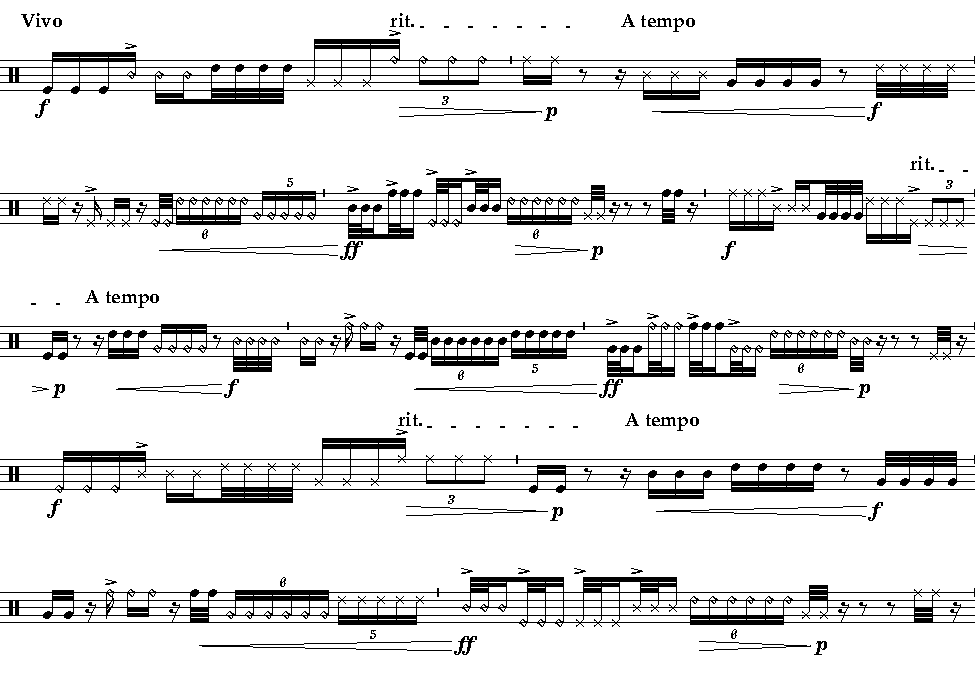
\includegraphics[width=6.5in]{figures/Example_Percussion.pdf}
\caption[Using self-derivation in a percussion setup.]{Using self-derivation to change instruments in a percussion setup.}
\label{fig:percussion}
\end{figure}

%TODO Add percussion key

%--------------------------------------------------------------------------
Each of the five instruments from each family is notated in Fig.~\ref{fig:percussion} in one of the staff lines, from bottom to top, according to ascending pitch. To discern between the instrument families, tom-toms are notated with a normal note head, cowbells with a diamond, and woodblocks with a cross. The base row $\{0, 2, 3, 1, 4\}$ in Listing~\ref{list:percussion} was chosen specifically not to be retrograde invariant. The set of solutions $\{37, 38, 39, 40\}$, on the other hand, was chosen to fit a particular musical structure. The semi-magic squares in solutions 37 and 38 are the same, and so are the semi-magic squares in solutions 39 and 40. The side vectors in solutions 37 and 38 differ by one row, whereas the side vectors in solutions 39 and 40 differ by two. Moreover, the side vectors in solutions 37 and 38 contain no representatives of the row class contained in the side vectors in solutions 39 and 40, and vice-versa. Therefore the entire passage can be broken into two statements. The motivation for this choice is to make the three repetitions of the basic rhythmic phrase as diverse as possible, avoiding any alignment between the repetitions and the solutions. This is accomplished by the fact that three is relatively prime to four and to two. Dynamics and tempo makings, nevertheless, are aligned with each repeated statement of the rhythmic phrase, since these two musical dimensions belong to the intuitive sphere of this musical composition.

%--------------------------------------------------------------------------
The next musical application is a passage for string quartet where four $4 \times 32$ combination matrices of self-derivation are used to determine pitch. The four instruments are associated with the four rows of the combination matrix in the canonical score order. An 8-tone row is used as the indices of an octatonic scale. The basic index row is $S = \{0, 2, 5, 6, 3, 1, 7, 4\}$. Listing~\ref{list:quartet} displays the output of a modified version of Listing~\ref{writeSolutions} where the base row is $RT_4(S) = \{0, 3, 5, 7, 2, 1, 6, 4\}$. The octatonic row is $\mathcal{O} = \{0, 2, 4, 5, 6, 8, 10, 11\}$, so that $S \mapsto \mathcal{O}$ is the injective mapping
\begin{equation}
	0 \mapsto 0, 1 \mapsto 2, 2 \mapsto 4, 3 \mapsto 5, 4 \mapsto 6, 5 \mapsto 8, 6 \mapsto 10, 7 \mapsto 11 \enspace . 
\end{equation}

%--------------------------------------------------------------------------
The output of Listing~\ref{writeSolutions} presented in Listing~\ref{list:quartet} is shown as a musical score in Fig.~\ref{fig:quartet}. The chosen set of solutions is $\{86, 116, 161, 175\}$, and these choices were based mostly on how each semi-magic square explored all instruments. The musical realization is straightforward in regards to how the rows of the combination matrices are mapped to the four instruments. Rhythmically, the contents of the combination matrices are realized depending on the contents of each semi-magic square. Square cells equal to one, two or zero are realized as 8\textsuperscript{th}-notes or rests. Square cells equal to three are realized as 16\textsuperscript{th}-note triplets, cells equal to four are realized as 32\textsuperscript{nd}-notes, and cells equal to five and six are realized as 32\textsuperscript{nd}-note quintuplets and sextuplets, respectively. Cells equal to two are struck simultaneously as double-stops and prolonged as 32\textsuperscript{nd}-note sextuplet tremolos. The tremolo order is the same as the square cell order, and the tremolos have a left and right spacing of one 8\textsuperscript{th}-note, that is, tremolos begin one 8\textsuperscript{th}-note after the double-stop, and end one 8\textsuperscript{th}-note before the next non-empty square cell for that instrument. Tremolos are altogether omitted when there is not enough time for them, hence there needs to be at least three 8\textsuperscript{th}-note rests between a double-stop and the next non-empty cell, so that the tremolo may be surrounded by rests. Besides the tremolos, the remainder of the passage is mostly pointillistic. To emphasize this characteristic, single and double-stop 8\textsuperscript{th}-notes are marked with pizzicati. The time signature changes in this realization are also influenced by the combination matrices. Given the aforementioned durations for each square cell size, every combination matrix column corresponds in Fig.~\ref{fig:quartet} to a bar, such that the time signature of every bar is the sum of the durations of the column cell in the corresponding combination matrix.

%--------------------------------------------------------------------------
\begin{lstlisting}[basicstyle=\ttfamily\footnotesize,numbers=none,caption={Output of Listing~\ref{writeSolutions} for problem size four and row $\{0, 3, 5, 7, 2, 1, 6, 4\}$.},label={list:quartet}]

Solution 86:
     0  3  5  7  2  1  6  4  | 0  3  5  7  2  1  6  4  |
2  |             2           |       5  7              |
28 | 0                 6     |    3        2           | ...
23 |    3  5                 | 0              1  6  4  |
19 |          7     1     4  |                         |
   | 2  5  7  1  4  3  0  6  | 7  1  4  5  2  0  6  3  
   |          1  4  3  0  6  |                         | 62
   |    5  7                 |    1  4                 | 93
   | 2                       | 7                       | 101
   |                         |          5  2  0  6  3  | 106

Solution 116:
     0  3  5  7  2  1  6  4  | 0  3  5  7  2  1  6  4  |
14 |                   6     |    3                    |
30 |             2           | 0     5              4  | ...
19 |          7     1     4  |                         |
0  | 0  3  5                 |          7  2  1  6     |

   | 4  7  1  3  6  5  2  0  | 6  3  1  7  4  5  0  2  
   |                         |       1  7  4  5  0  2  | 50
   |    7  1  3  6           |                         | 67
   |                5  2  0  | 6  3                    | 109
   | 4                       |                         | 125

Solution 161:
     0  3  5  7  2  1  6  4  | 0  3  5  7  2  1  6  4  |
0  |                         | 0  3  5                 |
7  |                         |          7  2        4  | ...
26 |                   6  4  |                1        |
0  | 0  3  5  7  2  1        |                   6     |

   | 7  2  4  6  1  0  5  3  | 0  3  5  7  2  1  6  4  
   | 7  2                    |                1  6  4  | 24
   |          6  1  0  5  3  |                         | 27
   |                         | 0  3  5  7  2           | 85
   |       4                 |                         | 156

Solution 175:
     0  3  5  7  2  1  6  4  | 0  3  5  7  2  1  6  4  |
0  |                         | 0  3  5                 |
9  |                1  6     |                      4  | ...
22 |             2        4  |          7              |
0  | 0  3  5  7              |             2  1  6     |

   | 0  5  3  1  6  7  2  4  | 1  6  4  2  7  0  3  5  
   |                7  2     | 1  6  4                 | 24
   |                         |          2  7  0  3  5  | 85
   | 0  5  3  1  6           |                         | 90
   |                      4  |                         | 140
\end{lstlisting}

\vspace{-1pt}

%--------------------------------------------------------------------------
\begin{figure}[H]
\centering
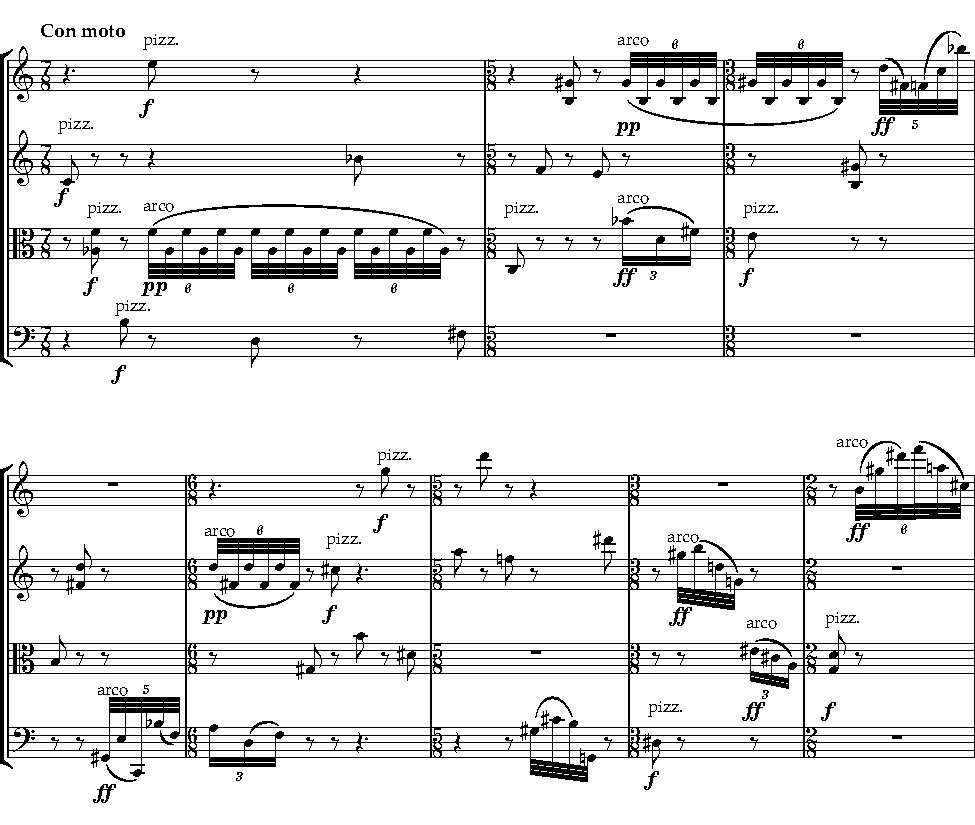
\includegraphics[width=6.5in]{figures/Example_Quartet_1.pdf}
\end{figure}

%--------------------------------------------------------------------------
\begin{figure}[H]
\centering
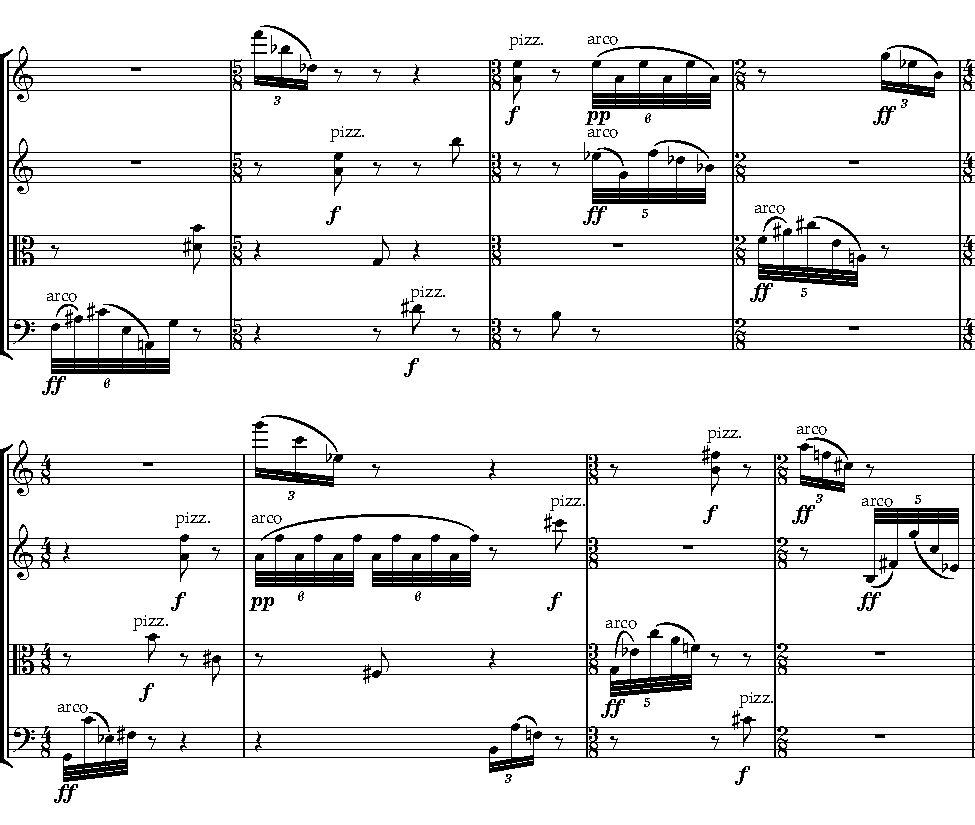
\includegraphics[width=6.5in]{figures/Example_Quartet_2.pdf}
\caption[Using self-derivation with an octatonic scale.]{Using self-derivation to map an octatonic scale to an 8-tone row.}
\label{fig:quartet}
\end{figure}

%TODO Add more musical examples

%--------------------------------------------------------------------------
\section{Conclusion}

%--------------------------------------------------------------------------
The algorithms, applications and examples presented in this dissertation represent an advancement in the study of combination matrices of self-derivation. Arguably the most notable contribution is an algorithm that is simple enough to allow computations by hand, while at the same time fast enough to generate thousands of solutions per second when run by a computer, and general enough to compute solutions for arbitrary problem and row sizes. The ideas in \cite{Starr1984} are invaluable for an understanding and classification of various derivation techniques from a set-theoretic perspective. They also contribute enormously to understanding how a particular class of solutions for the self-derivation problem can be constructed by exploring the permutation cycles of $RT_nI$ operations. What is missing in \cite{Starr1984} is an efficient way to compute combination matrices of self-derivation in a general setting. This shortcoming is addressed in \cite{Kowalski1987b}, which restricts its focus to the self-derivation problem and introduces an efficient algorithm to compute solutions for the 12-tone case. Even though the algorithm devised in \cite{Kowalski1987b} can be generalized to other row sizes, it is not a simple algorithm to understand or apply. More importantly, it intentionally avoids computing all possible solutions, sacrificing the less interesting ones for speed. The void that Listing~\ref{allSolutionsRecursive} intends to fill is exactly that of an algorithm that can produce a complete set of solutions given a row and a combination matrix size. The achieved result is straightforward to understand and implement. Devising this algorithm required understanding the problem of self-derivation from a new point-of-view, namely that of a structure that can be broken down into three basic constituent parts: a linearized top, a semi-magic square, and an array of derived row transforms. In this formulation, a top, a square and a side are necessary and sufficient to characterize a solution, that is, every solution is uniquely determined by them according to Th.~\ref{topSquareSideTheorem}. Such analysis of the problem paves the way for a much deeper understanding of self-derivation, especially when combined with a simple and fast algorithm capable of unveiling a large amount of solutions within reasonable time. Once the self-derivation problem was broken into parts, each part had to be studied and understood in detail. This study resulted in reducing the body of solutions into equivalence classes under the action of $RT_nI$, the number and sizes of which depending on the retrograde or retrograde inverse invariance of the row. This body of solutions also groups into classes of solutions which are equivalent under permutations of the side vector, leading to Cor.~\ref{topSquareSideCorollary}, and further into permutations of repeated semi-magic square rows. Although a significant advance, this paper is still a small step toward a more complete understanding of self-derivation, falling short in many aspects. Some of these aspects will be the subject of the rest of this chapter.

%--------------------------------------------------------------------------
\pagebreak
One major weakness of the present implementation is the way tops are pre-computed and stored as binary data. Although this method does improve execution speed, it is impractical, if not impossible, to handle large rows and problem sizes this way, as the number of possible tops becomes quickly unwieldy. One possibility to mitigate this problem would be to compute tops dynamically, compromising execution speed somewhat. In itself, this workaround would not help with the issue that Listing~\ref{allSolutionsRecursive} can produce an unmanageable amount of solutions, many if not most of them being rather uninteresting compositionally. There is a contradiction between a research goal in the present implementation, which is to devise an algorithm that produces a complete body of solutions, and the compositional goal of utilizing combination matrices to achieve meaningful counterpoint. Modifying the current implementation to focus on more interesting combination matrices is very easy, however. Besides the choice of row itself, the main contributor to uninteresting solutions is the semi-magic square itself. Therefore an implementation that restricts the search to squares capable of producing high merge indices should produce highly merged solutions according to the choice of row. Even though the current research is biased toward the understanding of self-derivation in all generality, the methodology described is still suitable for more restrictive applications. Restricting the range of the output of Listing~\ref{allSolutionsRecursive} may also represent a practical way of studying self-derivation itself in cases where the number of solutions is too large. This is an open topic of discussion, however, as what is considered too large is a matter of context. In a distributed system with hundreds of thousands of machines, space requirements and computational times have indeed a completely different meaning. Another argument is that improving how solutions can be further reduced into equivalence classes may involve first being able to produce all solutions. There are several additional ways in which the body of solutions produced by Listing~\ref{allSolutionsRecursive} may be amenable to reduction into representatives of larger and larger equivalence classes. One example is by allowing multiplication, that is, considering the action of the larger group $RT_nMI$. Multiplication in rows of arbitrary size generalizes to studying the group of automorphisms of $\mathbb{Z} / n \mathbb{Z}$, which in turn impacts how row classes are computed and retrograde invariances are filtered. Another example is to allow cyclic rotations of the row. Grouping rows into equivalence classes that include their cyclic rotations is thoroughly described in \cite{FripertingerLackner2015}. The compositional use of combination matrices of self-derivation that include cyclic-rotated transforms of the row can also be seen in \cite{Scotto2000}. Ex.~\ref{ex:scotto} shows how folding a $2 \times 24$ combination matrix of self-derivation into a $4 \times 48$ combination matrix can be achieved by simply repeating the top, that is, extending the top $\{T_0, RT_0\}$ into the top $\{T_0, RT_0, T_0, RT_0\}$. In Ex.~\ref{ex:scotto}, the derived rows contain cyclic-rotated transforms of the original row. Yet another example of how solutions may be reduced is given by how solutions for \emph{different} problem sizes can relate by the technique of folding, whether these relations contemplate cyclic-rotated transforms of the row or not. A particularly interesting consequence of regarding combination matrices of self-derivation as a top, a square and a side is that the set of semi-magic squares have some algebraic structure. It may be possible to reduce the set of solutions produced by Listing~\ref{allSolutionsRecursive} further, but more important could be the potential for generating musical syntax, as any operation that transforms a semi-magic square into another can motivate transforming a combination matrix into another. The action of $RT_nI$ on a combination matrix preserves the semi-magic square, therefore a transformation of the square itself may lead to more interesting musical syntax. Moreover, complete sets of solutions for a problem size and row can also help understanding how these solution sets relate for rows that are generated from the same aggregate realization, as described in \cite{Starr1984}. Comparing sets of solutions, however, brings out a fundamental problem with Listing~\ref{allSolutionsRecursive}, which is the fact that solutions are not output in a standardized order. Given an orbit of solutions under the action of $RT_nI$, a representative for the orbit may be picked by selecting the element where the first derived row is in canonical form. That would ensure that solution sets for different but related rows be more easily compared.

%--------------------------------------------------------------------------
Improving the present implementation may also be considered from the standpoint of execution speed and space requirements. The latter point would involve outputting solutions in a minimized form, such as top, square and side indices. A simple method similar to Listing~\ref{writeSolution} can then be used to reconstruct the solution as a combination matrix. The former point, that is, improving execution speed, is more involved. A simple optimization would be to use SIMD to vectorize vector addition and subtraction, which are fundamental components used in constructing and backtracking semi-magic squares. A more complicated possibility would be to use general purpose computing on the GPU to increase the number of threads. Although possible, this approach brings many complications. The most notable is that GPU programming is very suitable for applications where loops are broken down into into smaller ones and computed by multiple threads that load a single compute kernel. The recursive nature of Listing~\ref{allSolutionsRecursive} goes against this paradigm, and even though recursion is possible on the GPU, it is platform-specific and arguably not the best use of the GPU architecture. In fact, although GPU programming can be platform-independent to an extent, extracting every ounce of performance would likely involve getting into the implementation details of each platform. As mentioned previously, the use of distributed systems can greatly reduce computation times and make space constraints less problematic. It would also require less modifications to Listing~\ref{allSolutionsRecursive}, when compared to the GPU approach. At the same time, the code necessary to distribute the execution of Listing~\ref{allSolutionsRecursive} may be more platform-independent, and not require the modifications necessary to extract compute kernels from Listing~\ref{allSolutionsRecursive} and translate its recursive calls into iterative ones. The difficulty with distributed systems is either the access to a data center, or the cost of building one of a decent size. The use of self-derivation in real-time applications for electroacoustic music represents another area to which the ideas presented here can be extended. In these applications, the current execution speed of Listing~\ref{allSolutionsRecursive} may be adequate and no further optimizations be needed. By nature, combination matrices of self-derivation would fit best within a real-time music application in the sphere of event generation. That may or may not involve MIDI, but the more important observation is that generating events usually occurs at a much slower rate than the digital signal processing of audio samples. The modifications necessary to adapt Listing~\ref{allSolutionsRecursive} to a real-time application might involve not only how many combination matrices are output at a time, but also how these matrices are formatted. One idea is to pair each entry of the top with a timestamp. This vector of timestamps could be algorithmically generated, based on a time-point system, or even triggered by human interaction in live scenarios. Another idea is to pair each entry of each derived row with information regarding their register, if those are being used as pitch classes. Derived rows could also be marked with orchestration information, which in an electroacoustic context could mean the sound source triggered by an element of the derived row, with the derived row itself representing an entire track. For all these example applications, the changes to Listing~\ref{allSolutionsRecursive} would be minimal, and likely only involve adding parameters to it to restrict the output, as well as changing the output to a schematic representation of the combination matrix.

%--------------------------------------------------------------------------
This dissertation explored the concept of self-deriving combination matrices in a general setting. Derivation is a technique that was already used by Schoenberg, in conjunction with hexachordal combinatoriality \cite[100]{Westergaard1966}. The advancements made since Babbitt in the topic of general combinatoriality were reflected on the technique of derivation itself. Although incipient in \cite{Martino1961}, \cite{Westergaard1966} brings awareness to the possibility of working out by hand $12 \times 144$ combination matrices of self-derivation, and to the fact that more constrained problem sizes are harder to achieve. \cite{Starr1984} studies derivation and self-derivation from the standpoint of set theory, formalizing numerous procedures and devising three algorithms. \cite{Kowalski1987b} subsequently proposes a more general algorithm, focused on the problem of self-derivation. This dissertation expands on the ideas of Starr and Kowalski, proposing a novel algorithm that computes self-deriving combination matrices by separating the problem into a linearized top row, a side vector of self-derived rows, and an underlying semi-magic square. In the process, several mechanisms were devised with the intent to reduce the body of generated solutions into equivalence classes. Examples of the compositional application of self-deriving combination matrices were created to illustrate their use beyond the traditional 12-tone setting. The advancements made in the field of self-derivation are significant, but many directions for future research remain. Understanding how large bodies of solutions relate, both with equal and different problem sizes, such as in folded arrays, is a fundamental way to optimize performance and produce musical syntax.

%--------------------------------------------------------------------------
\section{Program Notes}

%--------------------------------------------------------------------------
\emph{Variations for Violoncello} is a short piece in three movements written for Craig Hultgren, who premiered it at the University of Florida on October 21\textsuperscript{st} of 2013, shortly after it was written. The piece explores the serial technique of self-derivation, in which several layers of coherence occur simultaneously. A set of rhythmic motivic cells is imposed over the pitch structures. These cells are constantly rotated, and evolve at an independent pace from the self-deriving pitch structures, whose syntax of row transforms stay somewhat constant. This procedure ultimately defines the impetus of the piece, where the quasi-kaleidoscopic nature of the pitch domain is driven by the ever free-spirited rhythmic motives.

%--------------------------------------------------------------------------
\emph{Out of Focus for Wind Quintet} is a short piece in a single movement with three contrasting sections. The piece departs from a generative algorithm which is stochastic in nature. Every instrument is centered around a particular note, and the algorithm dictates how these central notes evolve in terms of pitch and octave displacements, dynamics, and durations. The raw output of the algorithm is brought to life in a second and final compositional stage, where a myriad of adjustments and gestures are added to make the instruments sing. \emph{Out of Focus} was composed in 2014 and premiered as part of the Society of Composers, Inc. Showcase. The event took place at the University of Florida on February 7\textsuperscript{th} of 2015.

%--------------------------------------------------------------------------
The \emph{Duo for Alto Saxophone and Viola} is written in three movements, all drastically different from one another. The first movement explores the idea of permutation, concentrating almost obsessively on small collections of notes and exhausting their permutational possibilities. On top of this texture, the music unravels in the timbral and dynamical dimensions, producing long-winded phrases. The second movement is a most lyrical song, where the alto saxophone sings freely. The accompaniment is a sculpture \emph{da tirare}, where large blocks of harmony built over Perle-Lansky cycles are trimmed to satisfaction. A middle section is an adaptation of a famous (to some with my background) melody which I shall never reveal. Finally, the third movement is a fugue in which the note collections used for each section are expanding intervallic and rhythmic transforms of the initial statement. In other words, intervals as well as time signatures and motives get bigger up to a certain point, then shrink. Voices are carried and passed back and forth by both instruments, making this a very virtuosic fugue and concluding the piece with fireworks.

%--------------------------------------------------------------------------
\begin{figure}[htbp]
    \centering
	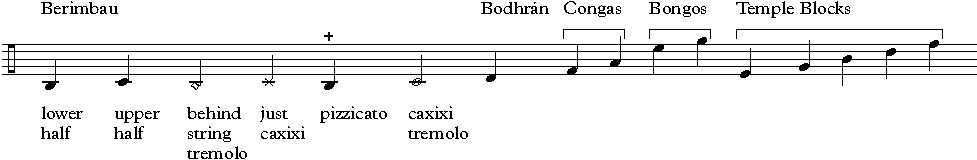
\includegraphics[width=6.5in]{figures/Percussion_Key.pdf}
	\caption[Percussion key for Damiani's \emph{Duo for Viola and Percussion}.]{Percussion key for Damiani's \emph{Duo for Viola and Percussion}.}
\end{figure}

%%--------------------------------------------------------------------------
\chapter{THEORETICAL FRAMEWORK}

This section proposes a model to describe derivation in a general setting. After writing the chapter, Luis will come back here and summarize what he wrote.

%--------------------------------------------------------------------------
\section{Defining an algorithm to compute a row class}

In a traditional setting, a composer will usually define a class of transforms of a basic row by computing by hand what is commonly termed as a 12-tone matrix. The general procedure is usually to fill the top row of the matrix with a transform of the row beginning with zero. The second step is to fill the leftmost column of the matrix with the inverse transform of the top row. The subsequent steps comprise going row-by-row and filling them with a transposition of the top row. The particular transposition for each row is the first pitch-class of the row. So if a row begins with, say, pitch-class $5$, then the entire row will be the $T_5$ transform of the top row. Then 12-tone matrix will hold all 48 transforms of a row: reading every row from left to right gives all transpositions, reading them from right to left gives all retrogrades, reading all columns from top to bottom gives all inversions, and reading them from bottom to top gives all retrograde inversions.

Although somewhat tedious, computing 12-tone matrices by hand is a well-established procedure. The 48 transforms that can be inferred from the matrix are not necessarily unique, given that a 12-tone may be retrograde, or retrograde-inverse invariant. It is straightforward to generalize the procedure to $n$-tone matrices. However, the graphical idea of reading the matrix from right to left, or bottom to top, is not ideal for computing self-deriving combination matrices, as it is faster to read a transform of a row that is written contiguously in memory. Another caveat is that the procedure does not necessarily define a canonical form for the top row. Every row in a matrix is a representative of an equivalence class of rows under the action of $RT_NI$. The size of each orbit is $4n$ if the row is not retrograde or retrograde-inverse invariant, and $2n$ otherwise. Defining a canonical form for the first row in a data structure that holds a row class is desirable in any algorithm that iterates through row classes in lexicographic order.

%--------------------------------------------------------------------------
\subsection{The canonical form of a row}

This section describes an algorithm to obtain a canonical form for a row. The canonical form defined here is simply the least element in a lexicographic ordering of a row class. Given an arbitrary representative of a row class, that representative will be considered retrograded if any interval class between two consecutive elements of the row, counted from right to left, is strictly less than the corresponding interval class counted from left to right. Finding the interval class between two pitch-classes is illustrated in Listing~\ref{intervalClass}, which takes as input two pitch-classes $a$ and $b$, and the base $n$, returning the interval class between the two. The interval class between $a \pmod n$ and $b \pmod n$ is expressed mathematically as $\min\{(a - b) \pmod n, (b - a) \pmod n\}$.

%--------------------------------------------------------------------------
\begin{lstlisting}[caption={Computing the interval class between two pitch-classes.},label={intervalClass}]
number intervalClass(number a, number b, number rowSize) {
    number interval = abs(a - b);
    return min(interval, rowSize - interval);
}
\end{lstlisting}

\begin{enumerate}
\item \emph{intervalClass} takes as input two pitch-classes $a$ and $b$, as well as the base $n$ so that $a, b \in \mathbb{Z} / n \mathbb{Z}$.
\item Line 2 simply computes the distance between $a$ and $b$.
\item Line 3 returns the least between the above interval and its complement, that is, the interval class between the two given pitch-classes.
\end{enumerate}

The procedure for determining whether a row is retrograded utilizes Listing~\ref{intervalClass} as a subroutine, and is outlined in Listing~\ref{isRetrograded}. The sole parameter to Listing~\ref{isRetrograded} is the row at hand, which can be any of the representatives of its row class, and the returned value is a boolean indicating whether the row is retrograded or not.

%--------------------------------------------------------------------------
\begin{lstlisting}[caption={Determining whether a representative of a row class is retrograded.},label={isRetrograded}]
bool isRetrograded(const number *row, number rowSize, bool isInvariant) {
    if (isInvariant || rowSize < 5)
        return false;

    number front, back;

    for (number i = 0; i < rowSize; ++i) {
        front = intervalClass(row[i + 1], row[i], rowSize);
        back = intervalClass(row[rowSize - i - 1], row[rowSize - i - 2], rowSize);

        if (back < front)
            return true;
    }

    return false;
}
\end{lstlisting}

\begin{enumerate}
\item \emph{isRetrograded} has three parameters, namely a pointer to a row, its size, and a boolean representing whether the row is retrograde or retrograde inverse-invariant.
\item Lines 2 and 3 perform a straightforward sanity check. It will be shown below that all rows of size 4 or less are necessarily retrograde or retrograde-invariant. If a row with 5 or more elements is known to be invariant, we skip the test.
\addtocounter{enumi}{2}
\item Line 5 declares the variables that will represent interval classes seen from left to right, and from right to left, respectively.
\addtocounter{enumi}{2}
\item Lines 8 and 9 simply update the variables front and back using Listing~\ref{intervalClass} defined above. As $i$ increases, front traverses all interval classes in the row from left to right, whereas back does the same from right to left, that is, back looks at the row as if it were retrograded.
\addtocounter{enumi}{2}
\item Line 11 compares the front and back interval classes and line 12 returns true if any interval class seen from right to left is strictly less than the corresponding interval class seen from left to right, which would indicate that retrograding the row would produce a lexicographically lower-positioned row than the one given as input.
\addtocounter{enumi}{3}
\item If all interval classes seen from both directions are equal, then the row is retrograde or retrograde inverse-invariant. Line 15 then returns false to avoid unnecessarily reversing a row that is invariant.
\end{enumerate}

The next step in determining the canonical form of a row consists of finding whether its inverse has a lower lexicographic position within the row class. The procedure is described in Listing~\ref{isInverted}, which in turn depends on two small subroutines, namely Listing~\ref{modulo} and Listing~\ref{isOwnInverse}. The former simply computes $modulo(x, n) = x \pmod{n}$. However, it needs to be defined in a subroutine this way because the result of C-language built-in modulo operator is signed, and for practical reasons that will be elaborated below, it is best that all pitch-classes be represented as unsigned integers ranging from $0$ to $n - 1$.

%--------------------------------------------------------------------------
\begin{lstlisting}[caption={A subroutine to compute $x \pmod{n}$ such that the result is non-negative.},label={modulo}]
number modulo(number x, number base) {
    x %= base;
    return x < 0 ? x + base : x;
}
\end{lstlisting}

\begin{enumerate}
\addtocounter{enumi}{1}
\item Line 2 simply computes $x \pmod{n}$ using the C-language built operator.
\item Line 3 then returns then same congruence class but in the range $[0, n - 1]$.
\end{enumerate}

Listing~\ref{isOwnInverse} is a simple convenience method that is used to check whether $x \equiv X \pmod{n}$, which is also needed in Listing~\ref{isInverted}.

%--------------------------------------------------------------------------
\begin{lstlisting}[caption={A subroutine that returns true if a pitch-class is its own inverse.},label={isOwnInverse}]
bool isOwnInverse(number x, number base) {
    return x == 0 || x == base - x;
}
\end{lstlisting}

\begin{enumerate}
\item The input $x$ is assumed to be in the range $[0, n - 1]$.
\item Since $x$ is non-negative, it can only be its own inverse if it is the identity, or if $x \equiv -x \pmod{n}$. It is also possible to check that if $n$ is even and $x$ is equal to $n / 2$, then $x$ is its own inverse. But this alternative method is far more computationally expensive that the one in Listing~\ref{isOwnInverse}.
\end{enumerate}

In order to determine whether the inverse transform of a row has a lower lexicographical position than itself, it is necessary in this implementation to consider if its retrograde transform also sits in a lower lexicographical position. The reason for that is because the input row has not been transformed at all up to this point. A prerequisite to calling Listing~\ref{isInverted} is to have previously called Listing~\ref{isRetrograded}, the result thereof being used as one of the inputs to Listing~\ref{isInverted}.

%--------------------------------------------------------------------------
\begin{lstlisting}[caption={Determining whether a representative of a row class is inverted.},label={isInverted}]
bool isInverted(const number *r, number rowSize, bool R) {
    if (R) {
        for (number i = rowSize - 1; i >= rowSize / 2; --i) {
            number mod = modulo(r[i] - r[rowSize - 1], rowSize);

            if (!isOwnInverse(mod, rowSize))
                return mod > rowSize - mod;
        }
    } else {
        for (number i = 0; i < rowSize / 2; ++i) {
            number mod = modulo(r[i] - r[0], rowSize);

            if (!isOwnInverse(mod, rowSize))
                return mod > rowSize - mod;
        }
    }

    return false;
}
\end{lstlisting}

\begin{enumerate}
\item The inputs are a row, its size, and a boolean representing whether the row is retrograded.
\addtocounter{enumi}{1}
\item If $r$ is retrograded, line 3 begins iteration in reverse order, that is, starting with the last element of the row.
\item Line 4 computes the ordered interval between the pitch-class at hand, and the first pitch-class of the row, which in this case is the last because the row is retrograded.
\addtocounter{enumi}{1}
\item Line 6 checks if the interval is not its own inverse and, if not, line 7 checks if the interval is greater than its inverse. If so, an inverted form of the row would sit in a lower lexicographical position within the entire row class, and the row is inverted.
\addtocounter{enumi}{3}
\item If the input row is not retrograded, then lines 10 to 14 perform essentially the same check as the previous branch, only traversing the row from left to right, instead of the right to left traversal done for a retrograded row. In both branches, it is important to note that the loops iterate at most twice. If the row size is odd, then the very first iteration will decide if the row is inverted. If, on the other hand, the row size is even, then there is the possibility that the very first interval will be its own inverse, in which case the next iteration will invariably be able to tell if the row is inverted.
\addtocounter{enumi}{7}
\item Line 18 should never be reached for well-defined inputs, and is included for correctness.
\end{enumerate}

Determining that an arbitrary representative of a row class is retrograded or inverted are essential subroutines used in Listing~\ref{getCanonicalForm}, which in turn does transform the input row into its canonical form. This transformation happens in Listing~\ref{getTransformInPlace}, and the latter relies on a straightforward method to in-place swap row entries, described below in Listing~\ref{swapInPlace}.

%--------------------------------------------------------------------------
\begin{lstlisting}[caption={Swapping two entries in a row.},label={swapInPlace}]
void swapInPlace(number *row, number i, number j) {
    number tmp = row[i];
    row[i] = row[j];
    row[j] = tmp;
}
\end{lstlisting}

The procedure in Listing~\ref{swapInPlace} is very common-place, so the details are omitted. Listing~\ref{getTransformInPlace} is also straightforward and represents the main subroutine in Listing~\ref{getCanonicalForm}.

%--------------------------------------------------------------------------
\begin{lstlisting}[caption={Transforming a row in place.},label={getTransformInPlace}]
void getTransformInPlace(number *row, number rowSize, number T, bool I, bool R) {
    if (R) {
        for (number i = 0; i < rowSize / 2; ++i)
            swapInPlace(row, i, rowSize - 1 - i);
    }

    if (I) {
        for (number i = 0; i < rowSize; ++i)
            row[i] = (rowSize - row[i] + T) % rowSize;
    } else if (T != 0 % rowSize) {
        for (number i = 0; i < rowSize; ++i)
            row[i] = (row[i] + T) % rowSize;
    }
}
\end{lstlisting}

\begin{enumerate}
\item The inputs are a row, its size, a non-negative integer representing an offset to be added to the entire row, a boolean representing whether the row is inverted, and another boolean representing whether the row is retrograded.
\addtocounter{enumi}{1}
\item If the row is retrograded, lines 3 and 4 simply reverse the row using Listing~\ref{swapInPlace}.
\addtocounter{enumi}{4}
\item If the row is inverted, lines 8 and 9 invert the row and add the offset to each row entry.
\addtocounter{enumi}{2}
\item Otherwise, if the row is not inverted, lines 11 and 12 only add the offset to the entire row.
\end{enumerate}

The procedure illustrated in Listing~\ref{getTransformInPlace} is used below in Listing~\ref{getCanonicalForm}, but it will also be used many times over to construct a row class in memory. In the particular case where the canonical form of the row is desired, that is, the lowest element in a lexicographical ordering of the row class, the offset used will be the additive inverse of the row's first element. It is important to observe that Listing~\ref{getCanonicalForm} requires prior knowledge as to whether the row is retrograde or retrograde inverse-invariant. In the grand scheme of things, that knowledge will already be available when calling Listing~\ref{getCanonicalForm}.

%--------------------------------------------------------------------------
\begin{lstlisting}[caption={Transforming a row into its canonical form.},label={getCanonicalForm}]
void getCanonicalForm(number *row, number rowSize, bool isInvariant) {
    bool R = isRetrograded(row, rowSize, isInvariant);
    bool I = isInverted(row, rowSize, R);
    number T = row[R ? rowSize - 1 : 0];
    getTransformInPlace(row, rowSize, I ? T : rowSize - T, I, R);
}
\end{lstlisting}

\begin{enumerate}
\item The inputs are a row, its size, and whether the row is retrograde or retrograde inverse-invariant.
\item Lines 2 and 3 simply call Listing~\ref{isRetrograded} and Listing~\ref{isInverted} respectively, storing the results.
\addtocounter{enumi}{1}
\item Line 4 just stores the first element of the row, which may be the last if the row is retrograded.
\item Line 5 is a call to Listing~\ref{getTransformInPlace}. The third argument is the additive inverse of the row's start element. It varies, naturally, if the row is inverted.
\end{enumerate}

%--------------------------------------------------------------------------
\subsection{Storing a row class in memory}

The purpose of the procedures described in this section is to store an entire row class contiguously in memory. That consists of creating an array large enough to hold all transforms of a row, and copying sequentially into this array said transforms. Even for rows whose base are considered large, a row class under $RTN_I$ is still very small. Thus holding these transforms in memory makes sense for execution speed purposes. The size of the row class array depends on whether the row is reverse or reverse inverse-invariant. The row class array begins with the canonical for of the row, followed by all its transpositions, in ascending order, followed by all transpositions of the inversion of the canonical for, also in ascending order. If the row is not reverse or reverse inverse-invariant, the row class array is appended by all transpositions of the reverse of the canonical order, followed by all transpositions of the retrograde inverse of the canonical order. Therefore, the overall size of the row class array is $2n^2$ if the row is retrograde or retrograde inverse-invariant, or $4n^2$ otherwise, where $n$ is the row size. The main routine for creating the row class array is described below in Listing~\ref{getRowClass}. It depends on two subroutines, namely Listing~\ref{isRetrogradeInvariant} and Listing~\ref{isRetrogradeInverseInvariant} that are described below.

%--------------------------------------------------------------------------
\begin{lemma}
	\label{retrograde-invariance}
	In a retrograde-invariant row, the interval between every entry seen from left to right, and the corresponding entry seen from right to left, must equal half the size of the row.
	\begin{proof}
	\end{proof}
\end{lemma}

%--------------------------------------------------------------------------
\begin{corollary}
	\label{odd-retrograde-invariance}
	A row with odd size greater than $3$ cannot be retrograde-invariant.
	\begin{proof}
	\end{proof}
\end{corollary}

%--------------------------------------------------------------------------
\begin{lstlisting}[caption={Determining whether a row is retrograde-invariant.},label={isRetrogradeInvariant}]
bool isRetrogradeInvariant(const number *row, number rowSize) {
    if (rowSize > 3 rowSize % 2 == 1)
        return false;

    number half = rowSize / 2;

    for (number i = 0; i < half; ++i) {
        if (modulo(row[rowSize - i - 1] - row[i], rowSize) != half)
            return false;
    }

    return true;
}
\end{lstlisting}

\begin{enumerate}
\item The only inputs are a row and its size.
\item Line 2 utilizes Th.~\ref{odd-retrograde-invariance} as a sanity check. If the test in line 2 succeeds, line 3 returns false.
\addtocounter{enumi}{2}
\item Line 5 just computes half the row size for convenience. Retrograde-invariance can be determined by iterating through at most half the size of the row.
\addtocounter{enumi}{1}
\item Line 7 iterates through the row from left to right, and line 8 applies Th.~\ref{retrograde-invariance}. Line 9 then returns false if any of the intervals is not equal to half the row size.
\addtocounter{enumi}{4}
\item If all pairs coming from both directions are equal to half the row size, then the row is retrograde-invariant and line 12 returns true.
\end{enumerate}

Unlike retrograde-invariance, every row size can produce retrograde inverse-invariance. A simple example is the lowest lexicographically-order row of any size, that is, a chromatic scale. Retrograding, inverting, and transposing by $-1$ always yields back the initial row. Listing~\ref{isRetrogradeInverseInvariant} outlines the procedure in all generality.

%TODO: when row size is odd, and all pairs sum to x, will the single element plus itself sum to x?

%--------------------------------------------------------------------------
\begin{lemma}
	\label{retrograde-inverse-invariance}
	In a retrograde inverse-invariant row $r$, the interval between every entry seen from left to right, and the corresponding entry seen from right to left, must be equal to $r_0 + r_{n - 1} \pmod{n}$, where $n$ is the base of the row.
	\begin{proof}
	\end{proof}
\end{lemma}

%--------------------------------------------------------------------------
\begin{lstlisting}[caption={Determining whether a row is retrograde inverse-invariant.},label={isRetrogradeInverseInvariant}]
bool isRetrogradeInverseInvariant(const number *row, number rowSize) {
    number half = rowSize / 2;
    number first = modulo(row[rowSize - 1] + row[0], rowSize);

    for (number i = 1; i < half; ++i) {
        if (modulo(row[rowSize - i - 1] + row[i], rowSize) != first)
            return false;
    }

    return true;
}
\end{lstlisting}

\begin{enumerate}
\item The inputs are a row and its size.
\item Line 2 computes half the row size for convenience. Like Listing~\ref{isRetrogradeInvariant}, retrograde inverse-invariance can be determined by traversing only half the row size.
\item Line 3 computes $r_0 + r_{n - 1} \pmod{n}$ for later use.
\addtocounter{enumi}{1}
\item Line 5 begins iteration from the second entry onward, since the first pair was already computed in line 3. Line 6 then compares the subsequent corresponding pairs, and line 7 returns false if any of them is not equal to the first pair.
\addtocounter{enumi}{4}
\item If line 10 is reached, it means the row is retrograde inverse-invariant, so the algorithm returns true.
\end{enumerate}

The procedure to compute and store an entire row class in memory is outlined below in Listing~\ref{getRowClass}. It returns a memory address that must be freed by the caller. While computing combination matrices of self-derivation, this memory location will be held for the duration of the program, and possibly also be shared by many different threads of execution. The procedure makes heavy use of Listing~\ref{getTransformInPlace} to sequentially store in memory all transforms of the canonical form of the row. It also takes the input row and transforms it in-place into its canonical form. Any representative of a row class can therefore be used to construct a row class with Listing~\ref{getRowClass}.

%--------------------------------------------------------------------------
\begin{lstlisting}[caption={Computing and storing a row class in memory.},label={getRowClass}]
number *getRowClass(range *classSize, number *row, number rowSize, bool isInvariant) {
    getCanonicalForm(row, rowSize, isInvariant);
    *classSize = isInvariant ? rowSize * 2 : rowSize * 4;

    number *rowClass = malloc(rowSize * *classSize * sizeof(number));
    memcpy(rowClass, row, rowSize * sizeof(number));

    for (number i = 1; i < rowSize; ++i) {
        number *rep = &rowClass[i * rowSize];
        memcpy(rep, rowClass, rowSize * sizeof(number));
        getTransformInPlace(rep, rowSize, i, false, false);
    }

    for (number i = rowSize; i < rowSize * 2; ++i) {
        number *rep = &rowClass[i * rowSize];
        memcpy(rep, rowClass, rowSize * sizeof(number));
        getTransformInPlace(rep, rowSize, i, true, false);
    }

    if (*classSize == rowSize * 2)
        return rowClass;

    for (number i = rowSize * 2; i < rowSize * 3; ++i) {
        number *rep = &rowClass[i * rowSize];
        memcpy(rep, rowClass, rowSize * sizeof(number));
        getTransformInPlace(rep, rowSize, i, false, true);
    }

    for (number i = rowSize * 3; i < rowSize * 4; ++i) {
        number *rep = &rowClass[i * rowSize];
        memcpy(rep, rowClass, rowSize * sizeof(number));
        getTransformInPlace(rep, rowSize, i, true, true);
    }

    return rowClass;
}
\end{lstlisting}

\begin{enumerate}
\item The inputs are a pointer to the size of the row class, which will be computed by Listing~\ref{getRowClass} and stored in the address provided, a row, its size, and a boolean representing whether the row is retrograde or retrograde inverse-invariant. This boolean will be computed by the caller before calling Listing~\ref{getRowClass}, utilizing the aforementioned procedures Listing~\ref{isRetrogradeInvariant} and Listing~\ref{isRetrogradeInverseInvariant}. The output is a memory location containing the entire row class.
\item As mentioned above, line 2 simply computes the canonical form of the given row in place.
\item Line 3 computes the class size based on whether the row is retrograde or retrograde inverse-invariant. It is important to notice here that the row class size is not the length of the row class array, but the number of transforms of the canonical form that the row class array contains. This number is stored in the address provided by the caller.
\addtocounter{enumi}{1}
\item Line 5 allocates in the heap the memory space that will be used to store the entire row class, and line 6 copies the canonical form of the row to the beginning of this allocated space.
\addtocounter{enumi}{2}
\item Line 8 starts from the second row in the row class, which is the first transposition of the canonical form, and the block adds all subsequent transpositions to the row class. Line 9 computes the address where the current transposition should start, line 10 copies the canonical for of the row into this address, and line 11 transforms the canonical for into the desired transposition in place. 
\addtocounter{enumi}{5}
\item Line 14 starts from the thirteenth row in the row class, that is, the $T_0I$ transform of the row. Lines 15 to 17 add the subsequent $T_nI$ transforms of the canonical for of the row in the same way the $T_n$ transforms were added above, only specifying in the call to Listing~\ref{getTransformInPlace} that the transforms now need to be inverted.
\addtocounter{enumi}{5}
\item Line 20 checks if the row is retrograde or retrograde inverse-invariant and, if so, halts the process and returns the memory location allocated in line 5.
\addtocounter{enumi}{2}
\item If the row is is retrograde or retrograde inverse-invariant, lines 23 to 26 add all $RT_n$ transforms of the row to the row class as above.
\addtocounter{enumi}{5}
\item Similarly, lines 29 to 32 add all the $RT_nI$ transforms of the row.
\addtocounter{enumi}{5}
\item Line 36 then simply returns the memory location allocated in line 5.
\end{enumerate}

%--------------------------------------------------------------------------
\section{Defining an algorithm to compute semi-magical squares}

A key component in the definition of a combination matrix of self-derivation is a semi-magic square. By definition, a semi-magic square is a square matrix where the sum of all elements, for each row and column, is a constant. For our purposes, that constant will be the base $n$ of the row. Seeing each entry in a semi-magic square as a real number and dividing each entry in the matrix by $n$ produces a doubly stochastic matrix, in which every row and every column sum to one. A magic square is a semi-magic square where, in addition, both main diagonals add up to the same constant as the rows and columns.

%--------------------------------------------------------------------------
\subsection{Computing the partitions of an integer}

By the definition above of a semi-magic square, every row therein is a permutation of an integer partition of $n$. In fact, every column is also a permutation of an integer partition of $n$, but the algorithm described below in Listing~\ref{allPartitionsRecursive} shall concentrate on computing all integer partitions of $n$ and their permutations as rows that will ultimately become the rows of a semi-magic square. Since these integer partitions of $n$ are completely independent of the row at hand, they can be computed only once for each $n$ and stored as a file, speeding up the process of computing combination matrices for other rows. Before describing Listing~\ref{allPartitionsRecursive}, a couple subroutines for reading and writing files are outlined.

%--------------------------------------------------------------------------
\begin{lstlisting}[caption={Retrieving the size of a file.},label={getFileSize}]
long getFileSize(FILE *file) {
    fseek(file, 0, SEEK_END);
    long fileSize = ftell(file);
    fseek(file, 0, SEEK_SET);
    return fileSize;
}
\end{lstlisting}

Listing~\ref{getFileSize} is a completely common-place procedure in the C-language, and its details are omitted. It is used as a subroutine in Listing~\ref{readFile}, which is described next.

%--------------------------------------------------------------------------
\begin{lstlisting}[caption={Reading the contents of a file.},label={readFile}]
number *readFile(const char *fileName, length *numLines, number problemSize) {
    FILE *file = fopen(fileName, "rb");

    if (file == NULL)
        return NULL;

    long fileSize = getFileSize(file);
    number *buffer = malloc(fileSize);
    *numLines = (length) (fileSize / sizeof(number)) / problemSize;
    fread(buffer, fileSize, 1, file);
    fclose(file);

    return buffer;
}
\end{lstlisting}

\begin{enumerate}
\item The inputs are the file name, assuming both the main executable and the file are in the same folder, a memory address where the number of lines read will be stored, and the problem size, which is the size of the magic square. The output is a memory location with the contents of the file, or a NULL pointer if the operation fails.
\item Line 2 simply opens the file at the given path for reading. Line 4 performs a sanity check and line 5 returns a NULL pointer if the file cannot be read.
\addtocounter{enumi}{4}
\item Line 7 is a call to Listing~\ref{getFileSize} so that the correct amount of memory can be allocated. The value computed in line 7 is already in bytes. Line 8 then allocates the memory whose address will be returned.
\addtocounter{enumi}{1}
\item Line 9 computes the number of lines in the file, that is, the number of integer partitions of $n$ with length \emph{problemSize} that have been previously computed and stored in the file. The value is then stored in the memory address provided in the input list to store the number of lines in the file.
\item Line 10 simply reads the entire contents of the file into the buffer allocated in line 8, line 11 frees the FILE data structure created in line 2, and line 13 returns the allocated memory. It is the responsibility of the caller to free this memory when no longer needed.
\end{enumerate}

The procedure described in Listing~\ref{writeAllPartitions} effectively writes all integer partitions of $n$ with a certain size to a file. It depends on Listing~\ref{allPartitionsRecursive} to compute all said partitions recursively, which is described next. One important feature of Listing~\ref{allPartitionsRecursive} is that it skips partitions whose all but one entries are zero. The reason for this is because the remaining entry would be forced to be equal to $n$. In any semi-magic square where there is an entry equal to $n$, both the row and column to which this entry belongs will necessarily contain only zeros except, of course, for the entry with value $n$. This means that the linearized top of the combination matrix at that semi-magic square's column will inevitably be trivially polyphonized, that is, the corresponding square cell would simply have the entire row at the top. Therefore any combination matrix can be extended by adding a column and a row at an arbitrary indices, and making that square entry contain $n$ elements, that is, a linearized statement of a row form. Since this procedure is completely general, the semi-magic squares computed below include entries only up to $n - 1$.

%--------------------------------------------------------------------------
\begin{lstlisting}[caption={Recursively computing all partitions of a number $n$ and permutations thereof with a certain size.},label={allPartitionsRecursive}]
void allPartitionsRecursive(number *tmp, number currentSize, number problemSize, number currentSum, number rowSize, FILE *file) {
    if (currentSize == problemSize - 1) {
        if (currentSum > 0) { // skip the [0, ..., 0, rowSize] partition
            tmp[currentSize] = rowSize - currentSum;
            fwrite(tmp, sizeof(number), problemSize, file);
        }

        return;
    }

    for (number i = 0; i < rowSize; ++i) {
        if (i + currentSum <= rowSize) {
            tmp[currentSize++] = i;
            allPartitionsRecursive(tmp, currentSize, problemSize, i + currentSum, rowSize, file);
            currentSize--;
        }
    }
}
\end{lstlisting}

\begin{enumerate}
\item The inputs are the address of some scratch memory previously allocated with the same length of the problem size, the current number of entries already placed in the scratch memory, the problem size, the current sum of the entries in the scratch memory, the base $n$, and a pointer to a FILE data structure where the partitions will be stored, line by line.
\item Line 2 deals with the base case of the recursion, that is, when the current number of elements in the scratch memory is one less than the problem size. If that is the case, then the last element in the scratch memory array must be equal to $n$ minus the sum of all previous elements.
\item Line 3 deals with the edge case where all entries up to problem size minus one are zero. That would force the very last element of the scratch memory array to be equal to $n$ which, by the discussion above is avoided in this implementation.
\item Line 4 sets the last element of the scratch memory array to $n$ minus the sum of its previous elements and line 5 writes the current partition to the given file. Having completed an entire partition, line 8 returns, so the function recurses no further.
\addtocounter{enumi}{6}
\item For the recursion cases where the scratch memory array has been filled with less than problem size minus one elements, the loop in line 11 iterates from zero to $n - 1$. Line 12 is a sanity check that the sum of the current element being appended to the scratch memory array with the current sum of all elements so far introduced is no greater than $n$. Line 13 then appends the current element to the end of the scratch memory array, increases the current size counter, and line 14 pushes to the call stack another recursive call to Listing~\ref{allPartitionsRecursive}.
\addtocounter{enumi}{1}
\item Line 15 backtracks the current size so that all combinations of integers in the range $[0, n - 1]$ are tried.
\end{enumerate}

Listing~\ref{writeAllPartitions} described below is essentially a wrapper around Listing~\ref{allPartitionsRecursive}. Partitions files are saved in the same location where the main executable is built, in order to facilitate dealing with file paths. In general, these files are very small even for large $n$, but the speed gains in precomputing them are worthwhile, given the recursive nature of Listing~\ref{allPartitionsRecursive}.

%--------------------------------------------------------------------------
\begin{lstlisting}[caption={Writing all partitions to a file.},label={writeAllPartitions}]
void writeAllPartitions(number problemSize, number rowSize) {
    char fileName[32];
    sprintf(fileName, "all_partitions_%i_%i.dat", problemSize, rowSize);
    FILE *file = fopen(fileName, "wb");

    number *tmp = malloc(problemSize * sizeof(number));
    allPartitionsRecursive(tmp, 0, problemSize, 0, rowSize, file);

    free(tmp);
    fclose(file);
}
\end{lstlisting}

\begin{enumerate}
\item The inputs are a problem size, which is the size of the semi-magic square, and a row size, which is the row base $n$.
\item Line 2 creates an array of 32 characters to hold the file name. This file name array length is large enough to accommodate all file names in this implementation. Line 3 writes the name of the file into the buffer defined in the previous line, and line 4 opens a C-type FILE for writing at the specified path.
\addtocounter{enumi}{3}
\item Line 6 allocates the scratch memory needed for the call to Listing~\ref{allPartitionsRecursive} in the following line. Being that Line 7 is the bottommost call on the call stack for Listing~\ref{allPartitionsRecursive}, the arguments given for the current size and current sum parameters are both zero.
\addtocounter{enumi}{2}
\item Line 9 frees the scratch memory used in the calls to Listing~\ref{allPartitionsRecursive}, and line 10 closes and releases the file created in line 4.
\end{enumerate}

The counterpart to Listing~\ref{writeAllPartitions} is Listing~\ref{readAllPartitions}, which is designed to not only read a partitions file, but to also generate one in case the particularly sought partitions file had not been previously created.

%--------------------------------------------------------------------------
\begin{lstlisting}[caption={Reading all partitions from a file.},label={readAllPartitions}]
number *readAllPartitions(length *numPartitions, number problemSize, number rowSize) {
    char fileName[32];
    sprintf(fileName, "all_partitions_%i_%i.dat", problemSize, rowSize);

    number *allPartitions = readFile(fileName, numPartitions, problemSize);

    if (allPartitions == NULL) {
        printf("Writing partitions file...\n");
        writeAllPartitions(problemSize, rowSize);
        allPartitions = readFile(fileName, numPartitions, problemSize);
    }

    return allPartitions;
}
\end{lstlisting}

\begin{enumerate}
\item The inputs are a memory address to store the number of lines in the partitions file to be read, the problem size and the row size. The output is a memory address with the contents of the partitions file. It is the responsibility of the caller to free the returned memory when no longer needed.
\item Lines 2 and 3 store the file name in a buffer, similarly to Listing~\ref{writeAllPartitions}.
\addtocounter{enumi}{2}
\item Line 5 attempts to read an existing file.
\addtocounter{enumi}{1}
\item Line 7 checks that the operation in line 5 succeeded. If it failed, lines 8 to 10 print to the console that a partitions file will be created, create the file by calling Listing~\ref{writeAllPartitions}, and attempt to read the file again.
\addtocounter{enumi}{5}
\item Line 13 simply returns the memory address with the contents of the file, or NULL if creating the file failed.
\end{enumerate}

%--------------------------------------------------------------------------
\subsection{Combining partition rows into squares}

This section describes an algorithm to combine integer partition rows into semi-magic squares. The overall procedure consists of appending integer partition rows to the square and adding the the rows as vectors. It is a backtracking recursive algorithm similar to Listing~\ref{allPartitionsRecursive}, the main difference being that the backtracking step consists of subtracting from the vector sum the previously added row after pushing onto the stack another recursive call. Adding two integer partition rows, seen as vectors, is described next in Listing~\ref{plus}.

%--------------------------------------------------------------------------
\begin{lstlisting}[caption={Adding two vectors.},label={plus}]
void plus(number *a, const number *b, number problemSize) {
    for (number i = 0; i < problemSize; ++i)
        a[i] += b[i];
}
\end{lstlisting}

\begin{enumerate}
\item The inputs are the memory locations of two vectors and their size, which assumed to be the same.
\item Line 2 simply iterates through the length of the vectors and line 3 adds point-wise the second vector to the first.
\end{enumerate}

The counterpart to Listing~\ref{plus} is Listing~\ref{minus}. It is important to notice that vector addition and subtraction can be vectorized for speed, that is, SIMD instructions from the processor architecture at hand can replace much of the work the for-loops in Listing~\ref{plus} is Listing~\ref{minus} do to great effect. This option is not explored in this implementation, however. Details are omitted for Listing~\ref{minus}, as is essentially the same as Listing~\ref{plus}, only with the inverse operation.

%--------------------------------------------------------------------------
\begin{lstlisting}[caption={Subtracting one vector from another.},label={minus}]
void minus(number *a, const number *b, number problemSize) {
    for (number i = 0; i < problemSize; ++i)
        a[i] -= b[i];
}
\end{lstlisting}

Listing~\ref{validate} is also used as subroutine in Listing~\ref{allSquaresRecursive} to validate whether the integer partition row that had just been added to the sum of rows vector does not violate the semi-magic square constraints.

%--------------------------------------------------------------------------
\begin{lstlisting}[caption={Validating a sum of integer partition rows.},label={validate}]
bool validate(const number *currentSum, number problemSize, number rowSize) {
    for (number i = 0; i < problemSize; ++i) {
        if (currentSum[i] > rowSize)
            return false;
    }

    return true;
}
\end{lstlisting}

\begin{enumerate}
\item The inputs are the memory location of the current sum of rows, the problem size, and the row size $n$.
\item Line 2 iterates through the size of the magic square, checking in line 3 whether any entry in the current sum vector is already greater than $n$, fact that would violate the semi-magic square definition. If so, line 4 returns false.
\addtocounter{enumi}{4}
\item If all entries in the current sum vector are less than or equal to $n$, this is still a viable semi-magic square, so line 7 returns true.
\end{enumerate}

Listing~\ref{allSquaresRecursive} utilizes the previously computed integer partition rows to form all possible semi-magic squares of size $n$, with entries in the range $[0, n - 1]$. It is described here because it facilitates understanding of Listing~\ref{allSolutionsRecursive}, but it is not used in computing combination matrices of self-derivation. For the latter purpose, computing \emph{all} possible semi-magical squares would be impractical, but this discussion is deferred to the next sections. Although Listing~\ref{allSquaresRecursive} takes as input a pointer to a FILE data structure, a procedure to save all semi-magic squares is omitted, as the number of such squares is overwhelmingly large and grows with both the problem size and $n$.

%--------------------------------------------------------------------------
\begin{lstlisting}[caption={Recursively computing all semi-magic squares of a certain size.},label={allSquaresRecursive}]
void allSquaresRecursive(number *tmp, number *currentSum, number currentSize, number problemSize, number rowSize, const number *partitions, length numPartitions, FILE *file) {
    if (currentSize == problemSize) {
        fwrite(tmp, sizeof(number), problemSize, file);
        return;
    }

    number start = 0;

    if (currentSize == 0)
        memset(currentSum, 0, problemSize * sizeof(number));
    else
        start = tmp[currentSize - 1];

    for (length i = start; i < numPartitions; ++i) {
        const number *p = &partitions[i * problemSize];
        plus(currentSum, p, problemSize);

        if (validate(currentSum, problemSize, rowSize)) {
            tmp[currentSize++] = i;
            allSquaresRecursive(tmp, currentSum, currentSize, problemSize, rowSize, partitions, numPartitions, file);
            currentSize--;
        }

        minus(currentSum, p, problemSize);
    }
}
\end{lstlisting}

\begin{enumerate}
\item The inputs are the memory address for some scratch memory where the semi-magical square will be stored as a sequence of indices into the integer partitions array. The size of this allocated memory must this be equal to the problem size. The memory address of another scratch memory space to hold the current sum of integer partition rows, with size equal to the problem size, the current number of rows already appended to the square, the problem size, the row size $n$, a pointer to the contents of a partitions file, previously computed using Listing~\ref{allPartitionsRecursive}, the total number of integer partition rows, and a pointer to a FILE data structure.
\item Line 2 deals with the base case of the recursion, that is, when all rows have been appended to the square. When that is the case, the algorithm writes the square to the file and returns.
\addtocounter{enumi}{4}
\item Line 7 defines a variable for where iteration of integer partition rows should start. This is a mechanism to avoid permutations of integer partition rows within a semi-magic square by enforcing that the rows of the constructed semi-magic square, seen as indices in the range between zero and the total number of integer partitions, be a nondecreasing sequence. The next section shall expand on the discussion of avoiding permutations of rows in semi-magical squares.
\addtocounter{enumi}{1}
\item Even though the current size is normally set to zero on a very first call to Listing~\ref{allSquaresRecursive}, the backtracking nature of the algorithm will push onto the call stack many other calls to Listing~\ref{allSquaresRecursive} where the current sum scratch memory might have been previously used, thus containing left over data. Line 9 then checks if the current size is zero, and line 10 sets all entries in the current sum scratch space to zero, to clear any left over data. If, on the other hand, the current size is greater than zero, then line 12 sets the start of the iteration to the very last index into the integer partition rows seen so far, guaranteeing that the sequence of indices in each square is nondecreasing.
\addtocounter{enumi}{4}
\item Line 14 begins iteration from the last index already in the square. In line 15, the variable \emph{p} stores the memory location of the integer partition row at the current index of iteration, and line 16 utilizes Listing~\ref{plus} to add this integer partition row to the current sum scratch memory.
\addtocounter{enumi}{3}
\item Line 18 calls Listing~\ref{validate} to validate the current sum and, if the sum is valid, line 19 sets the next index in the current square scratch memory, here represented by the variable \emph{tmp} to the current iteration index and increases the current size. Line 20 then pushes another call to Listing~\ref{allSquaresRecursive} onto the stack, and line 21 backtracks the current size.
\addtocounter{enumi}{5}
\item Regardless whether the validation test in line 18 succeeded, the current sum must be backtracked inside the same block where Listing~\ref{plus} was called. Line 24 accomplishes that with a balancing call to Listing~\ref{minus}.
\end{enumerate}

%--------------------------------------------------------------------------
\section{Computing all possible combination matrices for a row}

This section outlines a procedure that produces all combination matrices of self-derivation of a certain size for a particular row. The main idea relies on departing from a top row, which is a concatenation of transforms of the canonical form of a row $r$. If the row size is $n$, and the problem size is $m$, then the size of the top row is $m \times n$. In terms of derivation theory, the top row is completely linearized, and each of its $m$ transforms of the row $r$ will constitute a column of the combination matrix, if a solution for the top exists. The top itself is not part of the combination matrix, but rather the linearization thereof. It is, nonetheless, the point of departure of the main algorithm in this implementation. The combination matrix per se consists of a semi-magic square of size $m$ by $m$, where each column in the square defines a partition of the transform of $r$ for the corresponding section of the top. The last component in this view of a combination matrix of self-derivation are the transforms of the row $r$ that can be derived from the top row as a whole from the integer partitions given by the rows of the semi-magic square. These derived rows are a column vector of size $m$ which are called the sides of the combination matrix.

\begin{example}
Let $S = \{ 3, 8, 1, 0, 9, 6, 4, 7, 10, 5, 2, 11 \}$ as in Ex.~\ref{topSquareSideExample} and consider the combination matrix of self-derivation in Eq.~\ref{topSquareSideEquation}. In it, the top vector is $[\T_7(S) | \R\T_2\I(S)]$, the side vector is $[S | \T_9\I(S)]^T$, and the semi-magic square is

	\begin{equation}
        \left[
        \begin{array}{c|c}
            6 & 6 \\
            \hline
            6 & 6
        \end{array}
        \right] \enspace.
    \end{equation}
    
The row $S$ is not in its canonical form. An application of Listing~\ref{getCanonicalForm} reveals that the canonical form of $S$ is in fact the row $r = \{0, 3, 6, 11, 8, 5, 7, 10, 1, 2, 9, 4\}$, so that $S = RT_{11}(r)$.
\end{example}

\begin{theorem}
	\label{topSquareSideTheorem}
	Let $r$ be a row. If a  solution exists for a combination of top, side and square, then it is unique.
	\begin{proof}
	Suppose there exist two different solutions for the same combination of top, side and square. Then each solution comprises a combination matrix of self-derivation, say $M_1$ and $M_2$. By assumption $M_1 \ne M_2$. Now consider the linearized top and the first row of $M_1$, which is a transform of $r$, say $S_1(r)$. Since $M_1$ is a solution, when $S_1(r)$ is partitioned using the partition scheme given by the first row of the square, each partition of $S_1(r)$ fits exactly under each column of the top. Each column of the top is totally ordered, and so is each partition of $S_1(r)$. So there is only one way in which one can fit under another. The same reasoning applies to the first row of $M_2$, and to all subsequent rows of $M_1$ and $M_2$. Hence it must be that $M_1 = M_2$ and the solution is unique, as desired.
	\end{proof}
\end{theorem}

%--------------------------------------------------------------------------
\subsection{Computing the side and top rows of a combination matrix}

%--------------------------------------------------------------------------
\begin{lstlisting}[caption={},label={allSidesRecursive}]
void allSidesRecursive(number *tmp, number currentSize, number problemSize, range classSize, FILE *file) {
    if (currentSize == problemSize) {
        fwrite(tmp, sizeof(number), problemSize, file);
        return;
    }

    number start = currentSize == 0 ? 0 : tmp[currentSize - 1];

    for (range i = start; i < classSize; ++i) {
        tmp[currentSize++] = i;
        allSidesRecursive(tmp, currentSize, problemSize, classSize, file);
        currentSize--;
    }
}
\end{lstlisting}

\begin{enumerate}
\addtocounter{enumi}{1}
\item 
\end{enumerate}

%--------------------------------------------------------------------------
\begin{lstlisting}[caption={},label={allTopsRecursive}]
void allTopsRecursive(number *tmp, number currentSize, number problemSize, range classSize, FILE *file) {
    if (currentSize == problemSize) {
        fwrite(tmp, sizeof(number), problemSize, file);
        return;
    }

    // FIXME: this implementation cannot produce the R|P top, for example.

    if (currentSize == 0)
        tmp[currentSize++] = 0;

    for (range i = 0; i < classSize; ++i) {
        tmp[currentSize++] = i;
        allTopsRecursive(tmp, currentSize, problemSize, classSize, file);
        currentSize--;
    }
}
\end{lstlisting}

\begin{enumerate}
\addtocounter{enumi}{1}
\item 
\end{enumerate}

%--------------------------------------------------------------------------
\begin{lstlisting}[caption={},label={writeAllTops}]
void writeAllTops(number problemSize, range classSize) {
    char fileName[NAME_SIZE];
    sprintf(fileName, TOPS_FILE, problemSize, classSize);
    FILE *file = fopen(fileName, "wb");

    number *tmp = malloc(problemSize * sizeof(number));
    allTopsRecursive(tmp, 0, problemSize, classSize, file);

    free(tmp);
    fclose(file);
}
\end{lstlisting}

\begin{enumerate}
\addtocounter{enumi}{1}
\item 
\end{enumerate}

%--------------------------------------------------------------------------
\begin{lstlisting}[caption={},label={readAllTops}]
number *readAllTops(length *numTops, number problemSize, range classSize) {
    char fileName[NAME_SIZE];
    sprintf(fileName, TOPS_FILE, problemSize, classSize);

    number *allTops = readFile(fileName, numTops, problemSize);

    if (allTops == NULL) {
        printf("Writing top combos file...\n");
        writeAllTops(problemSize, classSize);
        allTops = readFile(fileName, numTops, problemSize);
    }

    return allTops;
}
\end{lstlisting}

\begin{enumerate}
\addtocounter{enumi}{1}
\item 
\end{enumerate}

%--------------------------------------------------------------------------
\subsection{Writing a solution as text}

%--------------------------------------------------------------------------
\begin{lstlisting}[caption={},label={writeRow}]
void writeRow(const number *row, number rowSize, range topSize, bool newLine, FILE *file) {
    for (range i = 0; i < topSize; ++i) {
        if (i > 0 && i % rowSize == 0)
            write(file, "| ");

        if (row[i] < 0)
            write(file, "   ");
        else if (row[i] < 10)
            write(file, "%i  ", row[i]);
        else
            write(file, "%i ", row[i]);
    }

    if (newLine)
        write(file, "\n");
}
\end{lstlisting}

\begin{enumerate}
\addtocounter{enumi}{1}
\item 
\end{enumerate}

%--------------------------------------------------------------------------
\begin{lstlisting}[caption={},label={writeSolution}]
void writeSolution(thread_data *d, common_data *cd, FILE *solutionsFile) {
    if (cd->problemSize > 0) {
        for (number k = 0; k < cd->problemSize; ++k) {
            write(solutionsFile, "%i ", d->tmpSide[k]);
            const number *p = &cd->allPartitions[d->tmpSquare[k] * cd->problemSize];

            for (int i = 0; i < cd->problemSize; ++i)
                write(solutionsFile, "%i ", p[i]);
        }

        write(solutionsFile, "\n");
        return;
    }

    write(solutionsFile, "Solution %lu:\n\n     ", d->counter);
    writeRow(d->tmpTops, cd->rowSize, cd->topSize, true, solutionsFile);

    for (number i = 0; i < cd->problemSize; ++i) {
        range topIndex = 0;
        number rowIndex = 0;
        const number *p = &cd->allPartitions[d->tmpSquare[i] * cd->problemSize];
        const number *r = &cd->rowClass[d->tmpSide[i] * cd->rowSize];
        memset(d->currentTop, -1, cd->topSize * sizeof(number));

        for (number j = 0; j < cd->problemSize; ++j) {
            number pj = p[j];

            for (range k = topIndex; k < topIndex + cd->rowSize; ++k) {
                if (pj == 0)
                    break;

                if (d->tmpTops[k] == r[rowIndex]) {
                    d->currentTop[k] = r[rowIndex];
                    rowIndex++;
                    pj--;
                }
            }

            topIndex += cd->rowSize;
        }

        if (d->tmpSide[i] < 10)
            write(solutionsFile, "%i  | ", d->tmpSide[i]);
        else
            write(solutionsFile, "%i | ", d->tmpSide[i]);

        writeRow(d->currentTop, cd->rowSize, cd->topSize, false, solutionsFile);
        write(solutionsFile, "| %lu\n", d->tmpSquare[i]);
    }

    write(solutionsFile, "\n");
}
\end{lstlisting}

\begin{enumerate}
\addtocounter{enumi}{1}
\item 
\end{enumerate}

%--------------------------------------------------------------------------
\subsection{Computing all possible solutions for a given combination matrix}

%--------------------------------------------------------------------------
\begin{lstlisting}[caption={},label={matchRowWithTop}]
bool matchRowWithTop(number *top, const number *row, const number *partitions, number problemSize, number rowSize) {
    range topIndex = 0;
    number rowIndex = 0;

    for (number i = 0; i < problemSize; ++i) {
        number p = partitions[i];

        for (range j = topIndex; j < topIndex + rowSize; ++j) {
            if (p == 0)
                break;

            if (top[j] == row[rowIndex]) {
                top[j] = -1;
                rowIndex++;
                p--;
            }
        }

        if (p > 0)
            return false;

        topIndex += rowSize;
    }

    return rowIndex == rowSize;
}
\end{lstlisting}

\begin{enumerate}
\addtocounter{enumi}{1}
\item 
\end{enumerate}

%--------------------------------------------------------------------------
\begin{lstlisting}[caption={},label={allSolutionsRecursive}]
void allSolutionsRecursive(thread_data *d, common_data *cd, FILE *solutionsFile, number currentSize) {
    if (currentSize == cd->problemSize) {
        d->counter++;
        writeSolution(d, cd, solutionsFile);
        return;
    }

    length start = 0;

    if (currentSize > 0) {
        start = d->tmpSquare[currentSize - 1];
        memcpy(&d->tmpTops[currentSize * cd->topSize], d->currentTop, cd->topSize * sizeof(number));
    }

    for (length i = start; i < cd->numPartitions; ++i) {
        const number *p = &cd->allPartitions[i * cd->problemSize];
        plus(d->currentSum, p, cd->problemSize);

        if (validate(d->currentSum, cd->problemSize, cd->rowSize)) {
            d->tmpSquare[currentSize] = i;

            // If the previous square index is the same as the current square index,
            // then we don't start from zero. Instead, we start from the previous row index plus one.
            // The sequence of row indices can be strictly increasing, since equal indices produce
            // equal rows, which cannot both equally fit into the same partition scheme given by the
            // current square index, which is the same as the previous square index by assumption.

            number rowStart = 0;

            if (currentSize > 0 && start == i)
                rowStart = d->tmpSide[currentSize - 1] + 1;

            for (range j = rowStart; j < cd->classSize; ++j) {
                const number *r = &cd->rowClass[j * cd->rowSize];

                if (matchRowWithTop(d->currentTop, r, p, cd->problemSize, cd->rowSize)) {
                    d->tmpSide[currentSize++] = j;
                    allSolutionsRecursive(d, cd, solutionsFile, currentSize);
                    currentSize--;
                }

                memcpy(d->currentTop, &d->tmpTops[currentSize * cd->topSize], cd->topSize * sizeof(number));
            }
        }

        minus(d->currentSum, p, cd->problemSize);
    }
}
\end{lstlisting}

\begin{enumerate}
\addtocounter{enumi}{1}
\item 
\end{enumerate}

%--------------------------------------------------------------------------
\section{Creating work data for use in concurrent threads}

%--------------------------------------------------------------------------
\begin{lstlisting}[caption={},label={createCommonData}]
void createCommonData(common_data *cd, int argc, char *argv[]) {
    number problemSize = (number) strtol(argv[1], NULL, 10);
    number rowSize = argc - 2;
    number *row = malloc(rowSize * sizeof(number));

    for (number i = 0; i < rowSize; ++i)
        row[i] = (number) strtol(argv[i + 2], NULL, 10);

    cd->problemSize = problemSize;
    cd->rowSize = rowSize;
    cd->topSize = problemSize * rowSize;

    bool rInvariant = isRetrogradeInvariant(row, rowSize);
    bool riInvariant = isRetrogradeInverseInvariant(row, rowSize);

    cd->isInvariant = rInvariant || riInvariant;
    cd->rowClass = getRowClass(&cd->classSize, row, rowSize, cd->isInvariant);
    cd->rMap = malloc(cd->classSize * sizeof(number));
    cd->riMap = malloc(cd->classSize * sizeof(number));
    cd->allPartitions = readAllPartitions(&cd->numPartitions, problemSize, rowSize);
    cd->allTops = readAllTops(&cd->numTops, problemSize, cd->classSize);

    if (rInvariant) {
        for (int i = 0; i < rowSize; ++i)
            cd->rMap[i] = cd->rowClass[(i + 1) * rowSize - 1];

        for (int i = rowSize; i < cd->classSize; ++i)
            cd->rMap[i] = cd->rowClass[(i + 1) * rowSize - 1] + rowSize;
    } else {
        for (int i = 0; i < rowSize; ++i)
            cd->rMap[i] = cd->rowClass[(i + 1) * rowSize - 1] + rowSize;

        for (int i = rowSize; i < cd->classSize; ++i)
            cd->rMap[i] = cd->rowClass[(i + 1) * rowSize - 1];
    }

    for (int i = 0; i < cd->classSize; ++i)
        cd->riMap[i] = (cd->rMap[i] == 0 || cd->rMap[i] == rowSize)
                       ? modulo(cd->rMap[i] + rowSize, cd->classSize)
                       : modulo(-cd->rMap[i], cd->classSize);

    free(row);
}
\end{lstlisting}

\begin{enumerate}
\addtocounter{enumi}{1}
\item 
\end{enumerate}

%--------------------------------------------------------------------------
\begin{lstlisting}[caption={},label={destroyCommonData}]
void destroyCommonData(common_data *cd) {
    free(cd->rowClass);
    free(cd->rMap);
    free(cd->riMap);
    free(cd->allPartitions);
    free(cd->allTops);
}
\end{lstlisting}

\begin{enumerate}
\addtocounter{enumi}{1}
\item 
\end{enumerate}

%--------------------------------------------------------------------------
\begin{lstlisting}[caption={},label={createSolutionsFile}]
FILE *createSolutionsFile(number *row, number problemSize, number rowSize, length startTop, length endTop) {
    char fileName[64];
    sprintf(fileName, "all_solutions_%i", problemSize);
    char offset = problemSize < 10 ? 15 : 16;

    for (number i = 0; i < rowSize; ++i) {
        sprintf(&fileName[offset], "_%i", row[i]);
        offset += row[i] < 10 ? 2 : 3;
    }

    sprintf(&fileName[offset], "_%lu_%lu.txt", startTop, endTop);

    return fopen(fileName, "wt");
}
\end{lstlisting}

\begin{enumerate}
\addtocounter{enumi}{1}
\item 
\end{enumerate}

%--------------------------------------------------------------------------
\begin{lstlisting}[caption={},label={fillTop}]
void fillTop(thread_data *d, common_data *cd, const number *combo) {
    for (number i = 0; i < cd->problemSize; ++i)
        memcpy(&d->currentTop[i * cd->rowSize],
               &cd->rowClass[combo[i] * cd->rowSize],
               cd->rowSize * sizeof(number));
}
\end{lstlisting}

\begin{enumerate}
\addtocounter{enumi}{1}
\item 
\end{enumerate}

%--------------------------------------------------------------------------
\begin{lstlisting}[caption={},label={unseen}]
// 1. Compute the R or RI-transform of the top.
// 2. Transpose the above so it starts with zero.
// 3. Go from left to right and return true if:
//    3.1. There is an entry greater than the top or;
//    3.2. There are no entries less than the top, implying the top is R or RI-invariant.
bool unseen(const number *top, common_data *cd) {
    number last = cd->problemSize - 1;
    number offset = cd->rMap[top[last]];
    bool invert = offset >= cd->rowSize;

    if (invert)
        offset = cd->riMap[top[last]];

    for (number i = 1; i < cd->problemSize; ++i) {
        number front = top[i];
        number back = invert ? cd->riMap[top[last - i]] : cd->rMap[top[last - i]];

        if (back < cd->rowSize)
            back = modulo(back - offset, cd->rowSize);
        else {
            back = modulo(back - offset - cd->rowSize, cd->rowSize);
            back += cd->rowSize;
        }

        if (back > front)
            return true;
        else if (back < front)
            return false;
    }

    return true;
}
\end{lstlisting}

\begin{enumerate}
\addtocounter{enumi}{1}
\item 
\end{enumerate}

%--------------------------------------------------------------------------
\begin{lstlisting}[caption={},label={createThreadData}]
void createThreadData(thread_data *d, common_data *cd) {
    d->counter = 0;
    d->tmpSide = malloc(cd->problemSize * sizeof(number));
    d->currentTop = malloc(cd->topSize * sizeof(number));
    d->tmpTops = malloc(cd->problemSize * cd->topSize * sizeof(number));
    d->currentSum = malloc(cd->problemSize * sizeof(number));
    d->tmpSquare = malloc(cd->problemSize * sizeof(length));
}
\end{lstlisting}

\begin{enumerate}
\addtocounter{enumi}{1}
\item 
\end{enumerate}

%--------------------------------------------------------------------------
\begin{lstlisting}[caption={},label={destroyThreadData}]
void destroyThreadData(thread_data *d) {
    free(d->tmpSide);
    free(d->currentTop);
    free(d->tmpTops);
    free(d->currentSum);
    free(d->tmpSquare);
}
\end{lstlisting}

\begin{enumerate}
\addtocounter{enumi}{1}
\item 
\end{enumerate}

%--------------------------------------------------------------------------
\section{Defining a top-level procedure for computing all solutions for a given row class}

%--------------------------------------------------------------------------
\begin{lstlisting}[caption={},label={writeSolutions}]
length writeSolutions(thread_data *d, common_data *cd, length startTop, length endTop) {
    //printMatrix(cd->rowClass, cd->classSize, cd->rowSize);
    length topCounter = 0;

    FILE *solutionsFile = createSolutionsFile(&cd->rowClass[0], cd->problemSize, cd->rowSize, startTop, endTop);

#if 0
    for (int first = 0; first < cd->classSize; ++first)
    for (length i = startTop; i < endTop; ++i) {
        number *combo = &cd->allTops[i * cd->problemSize];
        combo[0] = first;
#else
    for (length i = 0; i < 124; i += cd->problemSize) {
        const number *combo = &combos[i];
#endif
        if (cd->isInvariant && !unseen(combo, cd))
            continue;

        fillTop(d, cd, combo);
        memcpy(d->tmpTops, d->currentTop, cd->topSize * sizeof(number));
        memset(d->currentSum, 0, cd->problemSize * sizeof(number));
        allSolutionsRecursive(d, cd, solutionsFile, 0);
        topCounter++;
    }

    fclose(solutionsFile);

    return topCounter;
}
\end{lstlisting}

\begin{enumerate}
\addtocounter{enumi}{1}
\item 
\end{enumerate}

%%--------------------------------------------------------------------------
\chapter{APPLICATIONS AND CONCLUSION}

%--------------------------------------------------------------------------
\begin{lstlisting}[caption={},label={}]
int main(int argc, char *argv[]) {
    if (argc < 3) {
        printf("Enter a problem size and a row!\n");
        return -1;
    }

    common_data commonData;
    createCommonData(&commonData, argc, argv);

    thread_data data;
    createThreadData(&data, &commonData);

    clock_t start = clock();
    writeSolutions(&data, &commonData, 0, commonData.numTops);

    printf("%f seconds elapsed.\n", ((double) (clock() - start)) / CLOCKS_PER_SEC);
    printf("%lu solutions found!\n", data.counter);

    destroyThreadData(&data);
    destroyCommonData(&commonData);

    return 0;
}
\end{lstlisting}

\begin{enumerate}
\item
\addtocounter{enumi}{1}
\end{enumerate}

%--------------------------------------------------------------------------
\begin{lstlisting}[caption={},label={}]
class thread_manager {
public:
    thread_manager(int argc, char *argv[]) : threadData(std::thread::hardware_concurrency()) {
        createCommonData(&commonData, argc, argv);

        for (auto &data: threadData)
            createThreadData(&data, &commonData);
    }

    ~thread_manager() {
        for (auto &data: threadData)
            destroyThreadData(&data);

        destroyCommonData(&commonData);
    }

    long long runThreads() {
        auto numThreads = threadData.size();

        auto doWork = [this, &numThreads](int i, length startTop, length endTop) {
            writeSolutions(&threadData[i], &commonData, startTop, endTop);
            std::lock_guard<std::mutex> lock(mutex);
            numThreads--;
            condition.notify_one();
        };

        length startTop = 0;
        length offset = commonData.numTops / numThreads;
        auto maxThreads = numThreads - 1;
        auto startTime = std::chrono::high_resolution_clock::now();

        for (auto i = 0; i < maxThreads; ++i) {
            std::thread(doWork, i, startTop, startTop + offset).detach();
            startTop += offset;
        }

        doWork(maxThreads, startTop, commonData.numTops);

        std::unique_lock<std::mutex> lock(mutex);
        condition.wait(lock, [&numThreads] { return numThreads == 0; });

        auto stopTime = std::chrono::high_resolution_clock::now();
        auto duration = std::chrono::duration_cast<std::chrono::milliseconds>(stopTime - startTime);

        return duration.count();
    }

    length getNumSolutions() const {
        length numSolutions = 0;

        for (auto &data: threadData)
            numSolutions += data.counter;

        return numSolutions;
    }

private:
    std::vector<thread_data> threadData;
    common_data commonData;
    std::mutex mutex;
    std::condition_variable condition;
};
\end{lstlisting}

\begin{enumerate}
\item
\addtocounter{enumi}{1}
\end{enumerate}

%--------------------------------------------------------------------------
\begin{lstlisting}[caption={},label={}]
int main(int argc, char *argv[]) {
    if (argc < 3) {
        printf("Enter a problem size and a row!\n");
        return -1;
    }

    thread_manager threadManager(argc, argv);
    std::cout << threadManager.runThreads() << " milliseconds elapsed." << std::endl;
    std::cout << threadManager.getNumSolutions() << " solutions found!" << std::endl;

    return 0;
}
\end{lstlisting}

\begin{enumerate}
\item
\addtocounter{enumi}{1}
\end{enumerate}

We conclude this section with a musical example of how self-derivation may be achieved in a $6 \times 144$ matrix by exploring the symmetries of an aggregate realization.

\begin{example}
    \label{ex:stingray}
    Consider the aggregate realization A.
    \begin{equation}
        A = \begin{tikzcd}
            & 0 \arrow[dddr] && 1 \arrow[dddr] & \\
            & 4 \arrow[ddr] && 5 \arrow[ddr] & \\
            & 8 \arrow[dr] && 9 \arrow[dr] & \\
            * \arrow[ur] \arrow[uur] \arrow[uuur] \arrow[dr] \arrow[ddr] \arrow[dddr] && * \arrow[ur] \arrow[uur] \arrow[uuur] \arrow[dr] \arrow[ddr] \arrow[dddr] && * \\
            & 11 \arrow[ur] && 10 \arrow[ur] & \\
            & 7 \arrow[uur] && 6 \arrow[uur] & \\
            & 3 \arrow[uuur] && 2 \arrow[uuur] &
        \end{tikzcd} \enspace.
    \end{equation}
    It is easily seen that $A$ is invariant under the set of operations $\Omega = \{ \T_0, \T_4, \T_8, \T_3\I, \T_7\I, \T_{11}\I \}$. Thus if $\rho \in \Toc(A)$, then also $\Omega_i(\rho) \in \Toc(A)$. It is also easy to see that $\R(\rho) \in \Toc(\R \circ \Omega_i(A))$. Now let $S = \{ 0, 1, 5, 8, 9, 4, 10, 3, 7, 6, 2, 11 \}$, and consider the combination matrix $\mathcal{A} = [\mathcal{A}_1 | \cdots | \mathcal{A}_6]$.
    \begin{equation}
        \mathcal{A} = \left[
        \begin{array}{cc|cc|cc|cc|cc|cc}
            0 & 1 & 5 & 8 & 9 & 4 & 10 & 3 & 7 & 6 & 2 & 11 \\
            4 & 5 & 9 & 0 & 1 & 8 & 2 & 7 & 11 & 10 & 6 & 3 \\
            8 & 9 & 1 & 4 & 5 & 0 & 6 & 11 & 3 & 2 & 10 & 7 \\
            11 & 10 & 6 & 3 & 2 & 7 & 1 & 8 & 4 & 5 & 9 & 0 \\
            7 & 6 & 2 & 11 & 10 & 3 & 9 & 4 & 0 & 1 & 5 & 8 \\
            3 & 2 & 10 & 7 & 6 & 11 & 5 & 0 & 8 & 9 & 1 & 4
        \end{array}
        \right] \enspace.
    \end{equation}
    By construction, every row of $\mathcal{A}$ is an $\Omega$-transform of $S$. Also by construction, every $\mathcal{A}_i$ is an instance of either $A$ or $\R(A)$, seen as a columnar aggregate, and thus $\Omega$-invariant. It follows we can derive a transform of $S$ from every $\mathcal{A}_i$. Since $\T_7(S) \in \Toc(\mathcal{A}_1)$ and $\R\T_0\I(S) \in \Toc(\mathcal{A}_2)$, we get the self-derivation matrix $X$.
    \begin{equation}
        X = \left[
        \begin{array}{cccccccccccc|cccccccccccc}
            &&&&& 11 && 10 &&&&&&& 6 &&&&& 3 &&&& \\
            &&&& 4 && 5 &&&&&&&&&& 9 &&&&&&& 0 \\
            &&& 3 &&&&& 2 &&&&& 10 &&&&&&&& 7 && \\
            && 0 &&&&&&& 1 &&&&&& 5 &&& 8 &&&&& \\
            & 8 &&&&&&&&& 9 && 1 &&&&&&&& 4 &&& \\
            7 &&&&&&&&&&& 6 &&&&&& 2 &&&&& 11 &
        \end{array}
        \right] \enspace.
    \end{equation}
    It is important to point out that, although we could extend the matrix $X$ to a $6 \times 144$ derivation matrix wherein all columns of $\mathcal{A}$ are presented, we could not do so with arbitrary transforms of $S$. Upon inspection, we see that the transforms of $S$ we can derive from $\mathcal{A}_1$ and $\mathcal{A}_5$ are in
    \begin{equation}
        \{ \T_3, \T_7, \T_{11}, \R\T_1, \R\T_5, \R\T_9, \T_0\I, \T_4\I, \T_8\I, \R\T_2\I, \R\T_6\I, \R\T_{10}\I \} \enspace.
    \end{equation}
    For the columns $\mathcal{A}_2, \mathcal{A}_3, \mathcal{A}_4$ and $\mathcal{A}_6$, we can derive transforms of $S$ that are in
    \begin{equation}
        \{ \T_1, \T_5, \T_9, \R\T_3, \R\T_7, \R\T_{11}, \T_2\I, \T_6\I, \T_{10}\I, \R\T_0\I, \R\T_4\I, \R\T_8\I \} \enspace.
    \end{equation}
    Rather than a hinderance, one could take advantage of this fact by exploring contrasting harmonic regions. Fig.~\ref{fig:stingray} shows a musical realization of $X$:
    \begin{figure}[htbp]
        \centering
        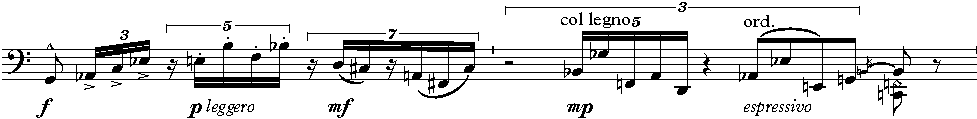
\includegraphics[width=6.5in]{figures/stingray-example.pdf}
        \caption[Self-derivation in Damiani's \emph{Stingray}.]{Self-derivation in Damiani's \emph{Stingray}.}
        \label{fig:stingray}
    \end{figure}
\end{example}

\subsection{Directions for the future}

Vectorize vector addition and subtraction.


%-----------------------------------------------------------------------%

% Use the appropriate file depending upon the number of appendices you have

%% The Editorial Office Requirements for the Table of Contents cause a significant problem
%in Latex if there is only one Appendix. The Appendix is no longer labeled "A" in the TOC
%but has the word "APPENDIX" placed in front of the title of the Appendix. This can be done
%without issue IF nothing needs to be numbered by LaTeX in the Appendix. Unfortunately, most of the time
%something needs to be numbered in that single Appendix. For this reason we have included the IFTHENELSE switch
%found in this document and at the beginning of AppendixA. We assume that if you have any appendices, that you have more than one. However, you DO only have one appendix DO NOT USE THIS FILE!!!!!!!!!!!!!!!!!!!!!!!
%
% OneSingleAppendix.tex has all the settings needed to adjust for a single appendix
% you will have a major problem with your TOC if you use this file with a single appendix!!!!!

%
% Comment (or delete) all of the \input{AppendixB} commands except those you are using.
%Then open the AppendixA.tex file and continue there.

%you can add/substract individual appendices through by using the /include{appendix'X'}
% and creating/deleting the appropriate files
\appendix %
%\clearpage%


\addtocontents{toc}{\protect\addvspace{10pt}\protect\noindent \protect APPENDIX}

% % % % % % % If you have a single appendix, you should be using appendix1.tex
% % % % % % % NOT this file

\chapter{THIS IS THE FIRST APPENDIX}

Lorem ipsum dolor sit amet, consectetuer adipiscing elit. Maecenas
eget magna. Aenean et lorem. Ut dignissim neque at nisi. In hac
habitasse platea dictumst. In porta ornare eros. Nunc eu ante. In
non est vehicula tellus cursus suscipit. Proin sed libero. Sed risus
enim, eleifend in, pellentesque ac, nonummy quis, nulla. Phasellus
imperdiet libero nec massa. Ut sapien libero, adipiscing eu,
volutpat porttitor, ultricies eget, nisi. Sed odio. Suspendisse
potenti. Duis dolor augue, viverra id, porta in, dignissim id, nisl.
Vivamus blandit cursus eros. Maecenas sit amet urna sit amet orci
nonummy pharetra.

Praesent cursus nibh et mauris. In aliquam felis sit amet ligula.
Nulla faucibus nisl eget nisl. Aliquam tincidunt. Mauris eget elit
sed massa luctus posuere. Pellentesque suscipit. In odio urna,
semper ut, convallis ut, porta et, nibh. Nulla sodales metus nec
velit posuere gravida. Cras tristique. Etiam urna risus, accumsan
ut, placerat sed, iaculis id, est.

Nullam mi. Pellentesque habitant morbi tristique senectus et netus
et malesuada fames ac turpis egestas. Duis vitae metus in massa
hendrerit rhoncus. Fusce tortor justo, laoreet eu, facilisis at,
gravida et, felis. Donec imperdiet mollis erat. Integer tempus nulla
ac lorem. Fusce porttitor. Aenean quis arcu. Morbi consectetuer, leo
eu mollis elementum, urna massa malesuada risus, euismod tempor
lorem elit ut mauris. Cras elit orci, facilisis ac, mattis iaculis,
cursus ac, augue. Donec eget nisl. Pellentesque fermentum sodales
nibh. Vivamus non risus. Donec est libero, tincidunt sit amet,
pretium vitae, blandit sed, tellus. Nunc diam risus, interdum sed,
laoreet quis, varius ac, turpis. In et purus eget nibh vehicula
rhoncus. Aenean et neque. Praesent nisl nisi, tempus quis, nonummy
ac, auctor a, neque. Suspendisse et metus. Suspendisse non metus eu
mauris auctor sagittis.
 %
\chapter{ELEMENTARY GROUP THEORY}

%\clearpage
%\thispagestyle{plain}
%\begin{landscape}
%\begin{figure}
%\begin{center}
%\includegraphics[width=6in]{images/LaTeX2e_logo.eps}
%\caption{\LaTeX 2\ensuremath{\epsilon.} logo}\label{biglogo}
%\end{center}
%\end{figure}
%\end{landscape}

\section{These are all the examples}

\ensuremath{\epsilon}

\begin{figure}[htbp]
\centering
\includegraphics[width=5in]{images/diagram} %[scale=1.0]
\caption[]{}
\end{figure}

\begin{table}[htbp]
\caption{A sample Table}\label{first}
\begin{tabularx}{6.5in}{XXX}
\hline
First & Second & Third \\
\hline
12 & 45 & 26 \\
17 & 32 & 93 \\
text & 51 & can be there too. \\	
\epsfig{figure=images/cat.eps, scale=1} & 28 & Figures too - a cat. \\
\begin{turn}{0}\epsfig{figure=images/mouse.eps, scale=0.25}\end{turn} & 000 & and a mouse! \\
\hline
\end{tabularx}
\end{table}

\begin{table}
\caption{Feasible triples for highly variable Grid, MLMMH.} \label{tbl1}
\begin{tabularx}{6.5 in}{r l X}
\hline {{Time (s)}} & {{Triple chosen}} & {{Other feasible triples}} \\ \hline
0 & (1, 11, 13725) & (1, 12, 10980), (1, 13, 8235), (2, 2, 0), (3, 1, 0) \\
2745 & (1, 12, 10980) & (1, 13, 8235), (2, 2, 0), (2, 3, 0), (3, 1, 0) \\
5490 & (1, 12, 13725) & (2, 2, 2745), (2, 3, 0), (3, 1, 0) \\
\hline
\end{tabularx}
\end{table}

\begin{table}[h!t!]
\begin{tabularx}{6.5 in}{r l X}
\multicolumn{3}{l}{Table \ref{tbl1}. Continued}\\%
\hline {{Time (s)}} & {{Triple chosen}} & {{Other feasible triples}} \\ \hline
115290 & (1, 13, 16470) & (2, 2, 2745), (2, 3, 0), (3, 1, 0) \\
118035 & (1, 13, 13725) & (2, 2, 2745), (2, 3, 0), (3, 1, 0) \\
120780 & (1, 13, 16470) & (2, 2, 2745), (2, 3, 0), (3, 1, 0) \\
123525 & (1, 13, 13725) & (2, 2, 2745), (2, 3, 0), (3, 1, 0) \\
\hline
\end{tabularx}
\end{table}
 %
\chapter{DERIVATION OF THE $\Upsilon$ FUNCTION}%
\label{appendixC}

%\clearpage %remove this command if your appendix doesn't start with a landscaped page!!!!!
%\thispagestyle{plain}
%\begin{landscape}
%\begin{figure}

 % \begin{center}
  %  \includegraphics[width=6in]{LaTeX2e_logo.eps}
   % \caption{\LaTeX 2\ensuremath{\epsilon.} logo}\label{biglogo}
  %\end{center}
%\end{figure}
%\end{landscape}

%%%%%%%%%%%%%%%%%%%%%%%%%%%%%%%%%%%%%%%%%%%%%%%%%%%%%%%%%%%%%%%%%%%%%%%%%%%%%%%%%%%%%%%%%%%%%%%%%%


%ADD LABEL

%%%%%%%%%%%%%%%%%%%%%%%%%%%%%%%%%%%%%%%%%%%%%%%%%%%%%%%%%%%%%%%%%%%%%%%%%%%%%%%%%%%%%%%%%%%%%%%%%%

\proposition{The Upsilon Function}\label{first}

(1) If $\beta>0$ and $\alpha\neq0$, then for all $n\geq-1$,

$$I_{n}(c;\alpha; \beta; \delta) = - \frac{e^{\alpha c}}{\alpha} \sum_{i=0}^{n}(\frac{\beta}{\alpha})^{n-i} Hh_{i}(\beta c -\delta)$$

$$+ (\frac{\beta}{\alpha})^{n+1} \frac{\sqrt{2 \pi}}{\beta} e^{\frac{\alpha \delta}{\beta}+\frac{\alpha^{2}}{2\beta^{2}}} \phi(-\beta c + \delta + \frac{\alpha}{\beta})$$
(2) If $\beta<0$ and $\alpha<0$, then for all $x \geq -1$

$$I_{n}(c;\alpha; \beta; \delta) = - \frac{e^{\alpha c}}{\alpha} \sum_{i=0}^{n}(\frac{\beta}{\alpha})^{n-i} Hh_{i}(\beta c -\delta)$$

$$- (\frac{\beta}{\alpha})^{n+1} \frac{\sqrt{2 \pi}}{\beta} e^{\frac{\alpha \delta}{\beta}+\frac{\alpha^{2}}{2\beta^{2}}} \phi(\beta c - \delta - \frac{\alpha}{\beta})$$

\begin{proof}{Case 1.}

$\beta>0$ and $\alpha\neq0$. Since, for any constant $\alpha$ and $n \geq 0$, $e^{\alpha x} Hh_{n}(\beta x - \delta) \rightarrow 0$ as $x \rightarrow \infty$ thanks to (B4), integration by parts leads to

$$I_{n}=-\frac{1}{\alpha}Hh(\beta c -\delta) e^{\alpha c} + \frac{\beta}{\alpha}\int_{c}^{\infty} e^{\alpha x} Hh_{n-1}(\beta c - \delta)dx$$

In other words, we have a recursion, for $n \geq 0$, $I_{n}=-(e^{\alpha c}{\alpha})Hh_{n}(\beta c - \delta) + (\frac{\beta}{\alpha})I_{n-1}$ with

$$I_{-1}=\sqrt{2 \pi} \int_{c}{\infty}e^{\alpha x}\varphi(-\beta x +\delta)dx$$

$$=\frac{\sqrt{2 \pi}}{\beta} e^{\frac{\alpha \delta}{\beta}+\frac{\alpha^{2}}{2 \beta^{2}}}\phi(-\beta c + \delta +\frac{\alpha}{\beta})$$

Solving it yields, for $n \geq -1$,

$$I_{n}=-\frac{e^{\alpha c}}{\alpha}\sum_{i=0}^{n}(\frac{\beta}{\alpha})^{i}Hh_{n-i}(\beta c+\delta) + (\frac{\beta}{\alpha})^{n+1}I_{-1}$$

$$=-\frac{e^{\alpha c}}{\alpha}\sum_{i=0}^{n}(\frac{\beta}{\alpha})^{n-i} Hh_{i}(\beta c+\delta)$$

$$+ (\frac{\beta}{\alpha})^{n+1}\frac{\sqrt{2 \pi}}{\beta} e^{\frac{\alpha \delta}{\beta}+\frac{\alpha^{2}}{2 \beta^{2}}}\phi(-\beta c + \delta +\frac{\alpha}{\beta})$$

where the sum over an empty set is defined to be zero.
\end{proof}

Case2. $\beta<0$ and $\alpha<0$. In this case, we must also have, for $n \geq 0$ and any constant $\alpha<0, e^{\alpha x}Hh_{n}(\beta x -\delta) \rightarrow 0$ as

$x \rightarrow \infty$, thanks to (B5). Using integration by parts, we again have the same recursion, for $n \geq 0, I_{n}=-(e^{\alpha c}/\alpha)Hh_{n}(\beta c - \delta)+(\beta / \alpha)I_{n-1}$, but with a different initial condition

$$I_{-1}=\sqrt{2 \pi}\int_{c}^{\infty}e^{\alpha x}\varphi(-\beta x + \delta)dx$$

$$=-\frac{\sqrt{2 \pi}}{\beta} exp\{\frac{\alpha \delta}{\beta}+\frac{\alpha^{2}}{2 \beta^{2}}\}\phi(\beta c - \delta -\frac{\alpha}{\beta})$$

Solving it yields (B8), for $n \geq -1$.

Finally, we sum the double exponential and the normal random variables

Proposition B.3.

Suppose $\{\xi_{1},\xi_{2},...\}$ is a sequence of i.i.d. exponential random variables with rate $\eta>0$, and Z is a normal variable with distribution $N(0,\sigma^{2})$. Then for every $ n \geq 1$, we have: (1) The density functions are given by:

$$f_{Z+\sum_{i=1}^{n}\xi_{i}}(t)=(\sigma\eta)^{n}\frac{e^{(\sigma\eta)^{2}/2}}{\sigma\sqrt{2\pi}}e^{-t\eta}Hh_{n-1}(-\frac{t}{\sigma}+\sigma\eta)$$

$$f_{Z-\sum_{i=1}^{n}\xi_{i}}(t)=(\sigma\eta)^{n}\frac{e^{(\sigma\eta)^{2}/2}}{\sigma\sqrt{2\pi}}e^{-t\eta}Hh_{n-1}(\frac{t}{\sigma}+\sigma\eta)$$
(2) The tail probabilities are given by

$$P(Z+\sum_{i=1}^{n}\xi_{i}\geq x) = (\sigma\eta)^{n}\frac{e^{(\sigma\eta)^{2}/2}}{\sigma\sqrt{2\pi}}e^{-t\eta}I_{n-1}(x;-\eta,-\frac{1}{\sigma},-\sigma\eta)$$

$$P(Z-\sum_{i=1}^{n}\xi_{i}\geq x) = (\sigma\eta)^{n}\frac{e^{(\sigma\eta)^{2}/2}}{\sigma\sqrt{2\pi}}e^{-t\eta}I_{n-1}(x;\eta,\frac{1}{\sigma},-\sigma\eta)$$

Proof. Case 1. The densities of $Z+\sum_{i=1}^{n}\xi_{i}$, and $Z-\sum_{i=1}^{n}\xi_{i}$. We have

$$f_{Z+\sum_{i=1}^{n}\xi_{i}}(t)=\int_{-\infty}^{\infty}f_{\sum_{i=1}^{n}\xi_{i}}(t-x)f_{Z}(x)dx$$

$$=e^{-t\eta}(\eta^{n})\int_{-\infty}{t}\frac{e^{x\eta}(t-x)^{n-1}}{(n-1)!}\frac{1}{\sigma\sqrt{2\pi}}e^{-x^{2}/(2\sigma^{2})}dx$$

$$=e^{-t\eta}(\eta^{n})e^{(\sigma\eta)^{2}/(2)}\int_{-\infty}{t}\frac{(t-x)^{n-1}}{(n-1)!}\frac{1}{\sigma\sqrt{2\pi}}e^{-(x-\sigma^{2}\eta)^{2}/(2\sigma^{2})}dx$$

Letting $y=(x-\sigma^{2}\eta)/\sigma$ yields

$$f_{Z+\sum_{i=1}^{n}\xi_{i}}(t)=e^{-t\eta}(\eta^{n})e^{(\sigma\eta)^{2}/(2)}\sigma^{n-1}$$

$$\times\int_{-\infty}^{t/\sigma-\sigma\eta}\frac{(t/\sigma - y -\sigma\eta)^{n-1}}{(n-1)!}\frac{1}{\sqrt{2\pi}}e^{-y^{2}/2}dy$$

$$=\frac{e^{(\sigma\eta)^{2}/2}}{\sqrt{2\pi}}(\sigma^{n-1}\eta^{n})e^{-t\eta}Hh_{n-1}(-t/\sigma + \sigma\eta)$$

because $(1/(n-1)!)\int_{-\infty}{a}(a-y)^{n-1}e^{-y^{2}/2}dy=Hh_{n-1}(a)$. The derivation of $f_{Z+\sum_{i=1}^{n}\xi_{i}}(t)$ is similar.

Case 2. $P(Z+\sum_{i=1}^{n}\xi_{i}\geq x)$ and $P(Z-\sum_{i=1}^{n}\xi_{i}\geq x)$. From (B9), it is clear that

$$P(Z+\sum_{i=1}^{n}\xi_{i}\geq x)=\frac{(\sigma\eta)^{n}e^{(\sigma\eta)^{2}/2}}{\sigma\sqrt{2\pi}}\int_{x}^{\infty}e^{(-i\eta)}Hh_{n-1}(-\frac{t}{\sigma}+\sigma\eta)dt$$

$$=\frac{(\sigma\eta)^{n}e^{(\sigma\eta)^{2}/2}}{\sigma\sqrt{2\pi}}I_{n-1}(x;-\eta,-\frac{1}{\sigma},-\sigma\eta)dt$$

by (B6). We can compute
$P(Z-\sum_{i=1}^{n}\xi_{i}\geq x)$ similarly.

\theorem{Theorem} With $\pi_{n}:= P(N(t)=n)=e^{-\lambda T}(\lambda T)^{n}/n!$ and $I_{n}$ in Proposition \ref{first}.
, we have

$$P(Z(T)\geq a)=\frac{e^{(\sigma \eta_{1})^{2} T/2}}{\sigma \sqrt{2 \pi T}} \sum_{n=1}^{\infty} \pi_{n} \sum_{k=1}^{n} P_{n,k}(\sigma\sqrt{T}\eta_{1})^{k}\times I_{k-1}(a-\mu T; -\eta_{1},-\frac{1}{\sigma\sqrt{T}},-\sigma\eta_{1}\sqrt{T})$$

$$+\frac{e^{(\sigma\eta_{2})^{2}T/2}}{\sigma\sqrt{2\pi T}}\sum_{n=1}^{\infty}\pi_{n}\sum_{k=1}^{n}Q_{n,k}(\sigma\sqrt{T}\eta_{2})^{k}$$

$$\times I_{k-1}(a-\mu T; \eta_{2},\frac{1}{\sigma\sqrt{T}},-\sigma\eta_{2}\sqrt{T})$$

$$+\pi_{0}\phi(-\frac{a-\mu T}{\sigma\sqrt{T}})$$

Proof by the decomposition (B2)

$$P(Z(T) \geq a)= \sum_{n=0}^{\infty}\pi_{n} P(\mu T +\sigma\sqrt{T} Z + \sum_{j=1}^{n}Y_{j} \geq a)$$

$$=\pi_{0}P(\mu T +\sigma\sqrt{T} Z  \geq a)$$

$$+\sum_{n=1}^{\infty}\pi_{n}\sum_{k=1}^{n}P_{n,k} P(\mu T +\sigma\sqrt{T} Z + \sum_{j=1}^{n}\xi_{j}^{+} \geq a)$$

$$+\sum_{n=1}^{\infty}\pi_{n}\sum_{k=1}^{n}Q_{n,k} P(\mu T +\sigma\sqrt{T} Z - \sum_{j=1}^{n}\xi_{j}^{-} \geq a)$$

The result now follows via (B11) and (B12) for $\eta_{1} > 1$ and $\eta_{2} >0$.


 %
\chapter{DERIVATION OF THE $\Upsilon$ FUNCTION}%
\label{appendixB}

%\clearpage %remove this command if your appendix doesn't start with a landscaped page!!!!!
%\thispagestyle{plain}
%\begin{landscape}
%\begin{figure}

% \begin{center}
  %  \includegraphics[width=6in]{LaTeX2e_logo.eps}
   % \caption{\LaTeX 2\ensuremath{\epsilon.} logo}\label{biglogo}
  %\end{center}
%\end{figure}
%\end{landscape}

%%%%%%%%%%%%%%%%%%%%%%%%%%%%%%%%%%%%%%%%%%%%%%%%%%%%%%%%%%%%%%%%%%%%%%%%%%%%%%%%%%%%%%%%%%%%%%%%%%

%ADD LABEL

%%%%%%%%%%%%%%%%%%%%%%%%%%%%%%%%%%%%%%%%%%%%%%%%%%%%%%%%%%%%%%%%%%%%%%%%%%%%%%%%%%%%%%%%%%%%%%%%%%

We first decompose the sum of the double exponential random variables.

The memoryless property of exponential random variables yields $(\xi^{+}-\xi^{-}|\xi^{+}>\xi^{-})=^{d}\xi^{+}$ and $(\xi^{+}-\xi^{-}|\xi^{+}<\xi^{-})=^{d}-\xi^{-}$, thus leading to the conclusion that

\begin{equation*}
\xi^{+}-\xi^{-} =\left\{
\begin{array}{rl}
\xi^{+} & \text{with probability $\eta_{2}/(\eta_{1}+\eta_{2})$ }\\
-\xi^{-} & \text{with probability $\eta_{1}/(\eta_{1}+\eta_{2})$ }
\end{array}\right\}.
\end{equation*}

because the probabilities of the events $\xi^{+}>\xi^{-}$ and $\xi^{+}<\xi^{-}$ are $\eta_{2}/(\eta_{1}+\eta_{2})$ and $\eta_{1}/(\eta_{1}+\eta_{2})$, respectively. The following proposition extends (B.1.)

Proposition B.1. For every $n\geq1$, we have the following decomposition

\begin{equation*}
\sum_{i=1}^{n}Y_{i}=^{d}\left\{
\begin{array}{rl}
\sum_{i=1}^{k}\xi_{i}^{+} & \text{with probability $P_{n,k},k=1,2,...,n$ }\\
-\sum_{i=1}^{k}\xi_{i}^{-} & \text{with probability $Q_{n,k},k=1,2,...,n$ }
\end{array}\right\}.
\end{equation*}

where $P_{n,k}$ and $Q_{n,k}$ are given by

$$P_{n,k}=\sum_{i=k}^{n-1}\binom {n-k-1} {i-k}\binom {n} {i}(\frac{\eta_{1}}{\eta_{1}+\eta_{2}})^{i-k}(\frac{\eta_{2}}{\eta_{1}+\eta_{2}})^{n-i}p^{i}q^{n-i}$$

$$1\leq k\leq n-1$$

$$Q_{n,k}=\sum_{i=k}^{n-1}\binom {n-k-1} {i-k}\binom {n} {i}(\frac{\eta_{1}}{\eta_{1}+\eta_{2}})^{n-i}(\frac{\eta_{2}}{\eta_{1}+\eta_{2}})^{i-k}p^{n-i}q^{i}$$

$$1\leq k\leq n-1, P_{n,n}=p^{n},Q_{n,n}=q^{n}$$

and $\binom{0}{0}$ is defined to be one. Hence $\xi_{i}^{+}$ and $\xi_{i}^{-}$ are i.i.d. exponential random variables with rates $\eta_{1}$ and $\eta_{2}$, respectively.

As a key step in deriving closed-form solutions for call and put options, this proposition indicates that the sum of the i.i.d. double exponential random variable can be written, in distribution, as a randomly mixed gamma random variable. To prove Proposition B.1, the following lemma is needed.

Lemma B.1.

$$\sum_{i=1}^{n}\xi_{i}^{+}-\sum_{i=1}^{n}\xi_{i}^{-}$$

\begin{equation*}
=^{d}\left\{
\begin{array}{rl}
\sum_{i=1}^{k}\xi_{i} & \text{with probability $\binom {n-k+m-1} {m-1}(\frac{\eta_{1}}{\eta_{1}+\eta_{2}})^{n-k}(\frac{\eta_{2}}{\eta_{1}+\eta_{2}})^{m}, k=1,...,n$ }\\
-\sum_{i=1}^{l}\xi_{i} & \text{with probability $\binom {n-l+m-1} {n-1}(\frac{\eta_{1}}{\eta_{1}+\eta_{2}})^{n}(\frac{\eta_{2}}{\eta_{1}+\eta_{2}})^{m-l}, l=1,...,m$ }
\end{array}\right\}.
\end{equation*}

We prove it by introducing the random variables $A(n,m) = \sum_{i=1}^{n}\xi_{i}-sum_{j=1}^{m}\tilde{\xi}_{j}$ Then

\begin{equation*}
A(n,m) =^{d}\left\{
\begin{array}{rl}
A(n-1,m-1)+\xi^{+} & \text{with probability $\eta_{2}/(\eta_{1}+\eta_{2})$ }\\
A(n-1,m-1)-\xi^{-} & \text{with probability $\eta_{1}/(\eta_{1}+\eta_{2})$ }
\end{array}\right\}.
\end{equation*}

\begin{equation*}
 =^{d}\left\{
\begin{array}{rl}
A(n,m-1) & \text{with probability $\eta_{2}/(\eta_{1}+\eta_{2})$ }\\
A(n-1,m) & \text{with probability $\eta_{1}/(\eta_{1}+\eta_{2})$ }
\end{array}\right\}.
\end{equation*}

via B.1.. Now suppose horizontal axis that are representing the number of $\{\zeta_{i}^{+}\}$ and vertical axis representing the number of $\{\zeta_{i}^{-}\}$. Suppose we have a random walk on the integer lattice points. Starting from any point $(n,m),n,m \geq 1$, the random walk goes either one step to the left with probability $\eta_{1}/(\eta_{1}+\eta_{2})$ or one step down with probability $\eta_{2}/(\eta_{1}+\eta_{2})$, and the random walks stops once it reaches the horizontal or vertical axis. For any path from (n,m) to (k,0) , $1 \geq k \geq n$, it must reach (k,1) first before it makes a final move to (k,0). Furthermore, all the paths going from (n,m) to (k,1) must have exactly n-k lefts and m-1 downs, whence the total number of such paths is $\binom {n-k+m-1}{m-1}$. Similarly the total number of paths from (n,m) to (0,l) , $1 \geq l \geq m$, is $\binom {n-l+m-1}{n-1}$. Thus

\begin{equation*}
A(n,m)=^{d}\left\{
\begin{array}{rl}
\sum_{i=1}^{k}\xi_{i} & \text{with probability $\binom {n-k+m-1} {m-1}(\frac{\eta_{1}}{\eta_{1}+\eta_{2}})^{n-k}(\frac{\eta_{2}}{\eta_{1}+\eta_{2}})^{m}, k=1,...,n$ }\\
-\sum_{i=1}^{l}\xi_{i} & \text{with probability $\binom {n-l+m-1} {n-1}(\frac{\eta_{1}}{\eta_{1}+\eta_{2}})^{n}(\frac{\eta_{2}}{\eta_{1}+\eta_{2}})^{m-l}, l=1,...,m$ }
\end{array}\right\}.
\end{equation*}

and the lemma is proven.

Now, let's prove the proposition B.1. By the same analogy used in Lemma B.1 to compute probability $P_{n,m},1\geq k \geq n$, the probability weight assigned to $\sum_{i=1}^{k}\xi_{i}^{+}$ when we decompose $\sum_{i=1}^{k}Y_{i}$, it is equivalent to consider the probability of the random walk ever reach (k,0) starting from the point (i,n-i) being $\binom {n}{i}p^{i}q^{n-i}$. Note that the point (k,0) can only be reached from point (i,n-i) such that $k \geq i \geq n-1$, because the random walk can only go left or down, and stops once it reaches the horizontal axis. Therefore, for $1 \geq k \geq n-1$, (B3) leads to

$$P_{n,k}=\sum_{i=k}{n-1}P(going from (i,n-i) to (k,0)). P(starting from (i,n-i))$$

$$=\sum_{i=k}^{n-1}\binom {i+(n-i)-k-1} {(n-i)-1}\binom {n} {i}(\frac{\eta_{1}}{\eta_{1}+\eta_{2}})^{i-k}(\frac{\eta_{2}}{\eta_{1}+\eta_{2}})^{n-i}p^{i}q^{n-i}$$

$$=\sum_{i=k}^{n-1}\binom {n-k-1} {n-i-1}\binom {n} {i}(\frac{\eta_{1}}{\eta_{1}+\eta_{2}})^{i-k}(\frac{\eta_{2}}{\eta_{1}+\eta_{2}})^{n-i}p^{i}q^{n-i}$$

$$=\sum_{i=k}^{n-1}\binom {n-k-1} {i-k}\binom {n} {i}(\frac{\eta_{1}}{\eta_{1}+\eta_{2}})^{i-k}(\frac{\eta_{2}}{\eta_{1}+\eta_{2}})^{n-i}p^{i}q^{n-i}$$

Of course $P_{n,n}=p^{n}$. Similarly, we can compute $Q_{n,k}$:

$$Q_{n,k}=\sum_{i=k}{n-1}P(going from (n-i,i) to (0,k)). P(starting from (n-i,i))$$

$$=\sum_{i=k}^{n-1}\binom {i+(n-i)-k-1} {(n-i)-1}\binom {n} {n-i}(\frac{\eta_{1}}{\eta_{1}+\eta_{2}})^{n-i}(\frac{\eta_{2}}{\eta_{1}+\eta_{2}})^{i-k}p^{n-i}q^{i}$$

$$=\sum_{i=k}^{n-1}\binom {n-k-1} {i-k}\binom {n} {i}(\frac{\eta_{1}}{\eta_{1}+\eta_{2}})^{n-i}(\frac{\eta_{2}}{\eta_{1}+\eta_{2}})^{i-k}p^{n-i}q^{i}$$

with $Q_{n,n}=q^{n}$. Incidentally, we have also got $\sum{k=1}{n}(P_{n,k}+Q_{n,k})=1$

B.2. Let's develop now the results on Hh functions.
First of all, note that $Hh_{n}(x)\rightarrow 0$, as $x \rightarrow \infty$, for $n \geq -1$; and $Hh_{n}(x) \rightarrow \infty$, as $x \rightarrow -\infty$, for $n \geq -1$; and $Hh_{0}(x)=\sqrt{2\pi} \phi(-x) \rightarrow \sqrt{2\pi}$, as $x \rightarrow -\infty$. Also, for every $n \geq -1$, as $x \rightarrow \infty$,

$$lim Hh_{n}(x)/\{\frac{1}{x^{n+1}}e^{-\frac{x^{2}}{2}}\}=1$$

and as $x \rightarrow \infty$

$$Hh_{n}(x)=O(|x|^{n})$$

Here (B4) is clearly true for $n=-1$, while for $n \geq 0$ note that as $x\rightarrow _\infty$,

$$Hh_{n}(x)=\frac{1}{n!}\int_{x}{\infty}(t-x)^{n}e^{-\frac{t^{2}}{2}}dt$$

$$\leq \frac{2^{n}}{n!}\int_{-\infty}^{\infty}|t|^{n}e^{-t^{2}}{2}dt+\frac{2^{n}}{n!}\int{-\infty}{\infty}|x|^{n}e^{-t^{2}}{2}dt=O(|x|^{n})$$

For option pricing it is important to evaluate the integral $I_{n}(c;\alpha;\beta;\delta)$,

$$I_{n}(c;\alpha;\beta;\delta)=\int_{c}{\infty}e^{\alpha x}Hh_{n}(\beta x-\delta)dx, n\geq 0$$

for arbitrary constants $\alpha, c$ and $\beta$.
 %
%\input{tex/appendixE} % %These files aren't included in the template
%\input{tex/appendixF} %
%\chapter{DERIVATION OF THE $\Upsilon$ FUNCTION}%
\label{appendixC}

%\clearpage %remove this command if your appendix doesn't start with a landscaped page!!!!!
%\thispagestyle{plain}
%\begin{landscape}
%\begin{figure}

 % \begin{center}
  %  \includegraphics[width=6in]{LaTeX2e_logo.eps}
   % \caption{\LaTeX 2\ensuremath{\epsilon.} logo}\label{biglogo}
  %\end{center}
%\end{figure}
%\end{landscape}

%%%%%%%%%%%%%%%%%%%%%%%%%%%%%%%%%%%%%%%%%%%%%%%%%%%%%%%%%%%%%%%%%%%%%%%%%%%%%%%%%%%%%%%%%%%%%%%%%%


%ADD LABEL

%%%%%%%%%%%%%%%%%%%%%%%%%%%%%%%%%%%%%%%%%%%%%%%%%%%%%%%%%%%%%%%%%%%%%%%%%%%%%%%%%%%%%%%%%%%%%%%%%%

\proposition{The Upsilon Function}\label{first}

(1) If $\beta>0$ and $\alpha\neq0$, then for all $n\geq-1$,

$$I_{n}(c;\alpha; \beta; \delta) = - \frac{e^{\alpha c}}{\alpha} \sum_{i=0}^{n}(\frac{\beta}{\alpha})^{n-i} Hh_{i}(\beta c -\delta)$$

$$+ (\frac{\beta}{\alpha})^{n+1} \frac{\sqrt{2 \pi}}{\beta} e^{\frac{\alpha \delta}{\beta}+\frac{\alpha^{2}}{2\beta^{2}}} \phi(-\beta c + \delta + \frac{\alpha}{\beta})$$
(2) If $\beta<0$ and $\alpha<0$, then for all $x \geq -1$

$$I_{n}(c;\alpha; \beta; \delta) = - \frac{e^{\alpha c}}{\alpha} \sum_{i=0}^{n}(\frac{\beta}{\alpha})^{n-i} Hh_{i}(\beta c -\delta)$$

$$- (\frac{\beta}{\alpha})^{n+1} \frac{\sqrt{2 \pi}}{\beta} e^{\frac{\alpha \delta}{\beta}+\frac{\alpha^{2}}{2\beta^{2}}} \phi(\beta c - \delta - \frac{\alpha}{\beta})$$

\begin{proof}{Case 1.}

$\beta>0$ and $\alpha\neq0$. Since, for any constant $\alpha$ and $n \geq 0$, $e^{\alpha x} Hh_{n}(\beta x - \delta) \rightarrow 0$ as $x \rightarrow \infty$ thanks to (B4), integration by parts leads to

$$I_{n}=-\frac{1}{\alpha}Hh(\beta c -\delta) e^{\alpha c} + \frac{\beta}{\alpha}\int_{c}^{\infty} e^{\alpha x} Hh_{n-1}(\beta c - \delta)dx$$

In other words, we have a recursion, for $n \geq 0$, $I_{n}=-(e^{\alpha c}{\alpha})Hh_{n}(\beta c - \delta) + (\frac{\beta}{\alpha})I_{n-1}$ with

$$I_{-1}=\sqrt{2 \pi} \int_{c}{\infty}e^{\alpha x}\varphi(-\beta x +\delta)dx$$

$$=\frac{\sqrt{2 \pi}}{\beta} e^{\frac{\alpha \delta}{\beta}+\frac{\alpha^{2}}{2 \beta^{2}}}\phi(-\beta c + \delta +\frac{\alpha}{\beta})$$

Solving it yields, for $n \geq -1$,

$$I_{n}=-\frac{e^{\alpha c}}{\alpha}\sum_{i=0}^{n}(\frac{\beta}{\alpha})^{i}Hh_{n-i}(\beta c+\delta) + (\frac{\beta}{\alpha})^{n+1}I_{-1}$$

$$=-\frac{e^{\alpha c}}{\alpha}\sum_{i=0}^{n}(\frac{\beta}{\alpha})^{n-i} Hh_{i}(\beta c+\delta)$$

$$+ (\frac{\beta}{\alpha})^{n+1}\frac{\sqrt{2 \pi}}{\beta} e^{\frac{\alpha \delta}{\beta}+\frac{\alpha^{2}}{2 \beta^{2}}}\phi(-\beta c + \delta +\frac{\alpha}{\beta})$$

where the sum over an empty set is defined to be zero.
\end{proof}

Case2. $\beta<0$ and $\alpha<0$. In this case, we must also have, for $n \geq 0$ and any constant $\alpha<0, e^{\alpha x}Hh_{n}(\beta x -\delta) \rightarrow 0$ as

$x \rightarrow \infty$, thanks to (B5). Using integration by parts, we again have the same recursion, for $n \geq 0, I_{n}=-(e^{\alpha c}/\alpha)Hh_{n}(\beta c - \delta)+(\beta / \alpha)I_{n-1}$, but with a different initial condition

$$I_{-1}=\sqrt{2 \pi}\int_{c}^{\infty}e^{\alpha x}\varphi(-\beta x + \delta)dx$$

$$=-\frac{\sqrt{2 \pi}}{\beta} exp\{\frac{\alpha \delta}{\beta}+\frac{\alpha^{2}}{2 \beta^{2}}\}\phi(\beta c - \delta -\frac{\alpha}{\beta})$$

Solving it yields (B8), for $n \geq -1$.

Finally, we sum the double exponential and the normal random variables

Proposition B.3.

Suppose $\{\xi_{1},\xi_{2},...\}$ is a sequence of i.i.d. exponential random variables with rate $\eta>0$, and Z is a normal variable with distribution $N(0,\sigma^{2})$. Then for every $ n \geq 1$, we have: (1) The density functions are given by:

$$f_{Z+\sum_{i=1}^{n}\xi_{i}}(t)=(\sigma\eta)^{n}\frac{e^{(\sigma\eta)^{2}/2}}{\sigma\sqrt{2\pi}}e^{-t\eta}Hh_{n-1}(-\frac{t}{\sigma}+\sigma\eta)$$

$$f_{Z-\sum_{i=1}^{n}\xi_{i}}(t)=(\sigma\eta)^{n}\frac{e^{(\sigma\eta)^{2}/2}}{\sigma\sqrt{2\pi}}e^{-t\eta}Hh_{n-1}(\frac{t}{\sigma}+\sigma\eta)$$
(2) The tail probabilities are given by

$$P(Z+\sum_{i=1}^{n}\xi_{i}\geq x) = (\sigma\eta)^{n}\frac{e^{(\sigma\eta)^{2}/2}}{\sigma\sqrt{2\pi}}e^{-t\eta}I_{n-1}(x;-\eta,-\frac{1}{\sigma},-\sigma\eta)$$

$$P(Z-\sum_{i=1}^{n}\xi_{i}\geq x) = (\sigma\eta)^{n}\frac{e^{(\sigma\eta)^{2}/2}}{\sigma\sqrt{2\pi}}e^{-t\eta}I_{n-1}(x;\eta,\frac{1}{\sigma},-\sigma\eta)$$

Proof. Case 1. The densities of $Z+\sum_{i=1}^{n}\xi_{i}$, and $Z-\sum_{i=1}^{n}\xi_{i}$. We have

$$f_{Z+\sum_{i=1}^{n}\xi_{i}}(t)=\int_{-\infty}^{\infty}f_{\sum_{i=1}^{n}\xi_{i}}(t-x)f_{Z}(x)dx$$

$$=e^{-t\eta}(\eta^{n})\int_{-\infty}{t}\frac{e^{x\eta}(t-x)^{n-1}}{(n-1)!}\frac{1}{\sigma\sqrt{2\pi}}e^{-x^{2}/(2\sigma^{2})}dx$$

$$=e^{-t\eta}(\eta^{n})e^{(\sigma\eta)^{2}/(2)}\int_{-\infty}{t}\frac{(t-x)^{n-1}}{(n-1)!}\frac{1}{\sigma\sqrt{2\pi}}e^{-(x-\sigma^{2}\eta)^{2}/(2\sigma^{2})}dx$$

Letting $y=(x-\sigma^{2}\eta)/\sigma$ yields

$$f_{Z+\sum_{i=1}^{n}\xi_{i}}(t)=e^{-t\eta}(\eta^{n})e^{(\sigma\eta)^{2}/(2)}\sigma^{n-1}$$

$$\times\int_{-\infty}^{t/\sigma-\sigma\eta}\frac{(t/\sigma - y -\sigma\eta)^{n-1}}{(n-1)!}\frac{1}{\sqrt{2\pi}}e^{-y^{2}/2}dy$$

$$=\frac{e^{(\sigma\eta)^{2}/2}}{\sqrt{2\pi}}(\sigma^{n-1}\eta^{n})e^{-t\eta}Hh_{n-1}(-t/\sigma + \sigma\eta)$$

because $(1/(n-1)!)\int_{-\infty}{a}(a-y)^{n-1}e^{-y^{2}/2}dy=Hh_{n-1}(a)$. The derivation of $f_{Z+\sum_{i=1}^{n}\xi_{i}}(t)$ is similar.

Case 2. $P(Z+\sum_{i=1}^{n}\xi_{i}\geq x)$ and $P(Z-\sum_{i=1}^{n}\xi_{i}\geq x)$. From (B9), it is clear that

$$P(Z+\sum_{i=1}^{n}\xi_{i}\geq x)=\frac{(\sigma\eta)^{n}e^{(\sigma\eta)^{2}/2}}{\sigma\sqrt{2\pi}}\int_{x}^{\infty}e^{(-i\eta)}Hh_{n-1}(-\frac{t}{\sigma}+\sigma\eta)dt$$

$$=\frac{(\sigma\eta)^{n}e^{(\sigma\eta)^{2}/2}}{\sigma\sqrt{2\pi}}I_{n-1}(x;-\eta,-\frac{1}{\sigma},-\sigma\eta)dt$$

by (B6). We can compute
$P(Z-\sum_{i=1}^{n}\xi_{i}\geq x)$ similarly.

\theorem{Theorem} With $\pi_{n}:= P(N(t)=n)=e^{-\lambda T}(\lambda T)^{n}/n!$ and $I_{n}$ in Proposition \ref{first}.
, we have

$$P(Z(T)\geq a)=\frac{e^{(\sigma \eta_{1})^{2} T/2}}{\sigma \sqrt{2 \pi T}} \sum_{n=1}^{\infty} \pi_{n} \sum_{k=1}^{n} P_{n,k}(\sigma\sqrt{T}\eta_{1})^{k}\times I_{k-1}(a-\mu T; -\eta_{1},-\frac{1}{\sigma\sqrt{T}},-\sigma\eta_{1}\sqrt{T})$$

$$+\frac{e^{(\sigma\eta_{2})^{2}T/2}}{\sigma\sqrt{2\pi T}}\sum_{n=1}^{\infty}\pi_{n}\sum_{k=1}^{n}Q_{n,k}(\sigma\sqrt{T}\eta_{2})^{k}$$

$$\times I_{k-1}(a-\mu T; \eta_{2},\frac{1}{\sigma\sqrt{T}},-\sigma\eta_{2}\sqrt{T})$$

$$+\pi_{0}\phi(-\frac{a-\mu T}{\sigma\sqrt{T}})$$

Proof by the decomposition (B2)

$$P(Z(T) \geq a)= \sum_{n=0}^{\infty}\pi_{n} P(\mu T +\sigma\sqrt{T} Z + \sum_{j=1}^{n}Y_{j} \geq a)$$

$$=\pi_{0}P(\mu T +\sigma\sqrt{T} Z  \geq a)$$

$$+\sum_{n=1}^{\infty}\pi_{n}\sum_{k=1}^{n}P_{n,k} P(\mu T +\sigma\sqrt{T} Z + \sum_{j=1}^{n}\xi_{j}^{+} \geq a)$$

$$+\sum_{n=1}^{\infty}\pi_{n}\sum_{k=1}^{n}Q_{n,k} P(\mu T +\sigma\sqrt{T} Z - \sum_{j=1}^{n}\xi_{j}^{-} \geq a)$$

The result now follows via (B11) and (B12) for $\eta_{1} > 1$ and $\eta_{2} >0$.


 
%\chapter{DERIVATION OF THE $\Upsilon$ FUNCTION}%
\label{appendixB}

%\clearpage %remove this command if your appendix doesn't start with a landscaped page!!!!!
%\thispagestyle{plain}
%\begin{landscape}
%\begin{figure}

% \begin{center}
  %  \includegraphics[width=6in]{LaTeX2e_logo.eps}
   % \caption{\LaTeX 2\ensuremath{\epsilon.} logo}\label{biglogo}
  %\end{center}
%\end{figure}
%\end{landscape}

%%%%%%%%%%%%%%%%%%%%%%%%%%%%%%%%%%%%%%%%%%%%%%%%%%%%%%%%%%%%%%%%%%%%%%%%%%%%%%%%%%%%%%%%%%%%%%%%%%

%ADD LABEL

%%%%%%%%%%%%%%%%%%%%%%%%%%%%%%%%%%%%%%%%%%%%%%%%%%%%%%%%%%%%%%%%%%%%%%%%%%%%%%%%%%%%%%%%%%%%%%%%%%

We first decompose the sum of the double exponential random variables.

The memoryless property of exponential random variables yields $(\xi^{+}-\xi^{-}|\xi^{+}>\xi^{-})=^{d}\xi^{+}$ and $(\xi^{+}-\xi^{-}|\xi^{+}<\xi^{-})=^{d}-\xi^{-}$, thus leading to the conclusion that

\begin{equation*}
\xi^{+}-\xi^{-} =\left\{
\begin{array}{rl}
\xi^{+} & \text{with probability $\eta_{2}/(\eta_{1}+\eta_{2})$ }\\
-\xi^{-} & \text{with probability $\eta_{1}/(\eta_{1}+\eta_{2})$ }
\end{array}\right\}.
\end{equation*}

because the probabilities of the events $\xi^{+}>\xi^{-}$ and $\xi^{+}<\xi^{-}$ are $\eta_{2}/(\eta_{1}+\eta_{2})$ and $\eta_{1}/(\eta_{1}+\eta_{2})$, respectively. The following proposition extends (B.1.)

Proposition B.1. For every $n\geq1$, we have the following decomposition

\begin{equation*}
\sum_{i=1}^{n}Y_{i}=^{d}\left\{
\begin{array}{rl}
\sum_{i=1}^{k}\xi_{i}^{+} & \text{with probability $P_{n,k},k=1,2,...,n$ }\\
-\sum_{i=1}^{k}\xi_{i}^{-} & \text{with probability $Q_{n,k},k=1,2,...,n$ }
\end{array}\right\}.
\end{equation*}

where $P_{n,k}$ and $Q_{n,k}$ are given by

$$P_{n,k}=\sum_{i=k}^{n-1}\binom {n-k-1} {i-k}\binom {n} {i}(\frac{\eta_{1}}{\eta_{1}+\eta_{2}})^{i-k}(\frac{\eta_{2}}{\eta_{1}+\eta_{2}})^{n-i}p^{i}q^{n-i}$$

$$1\leq k\leq n-1$$

$$Q_{n,k}=\sum_{i=k}^{n-1}\binom {n-k-1} {i-k}\binom {n} {i}(\frac{\eta_{1}}{\eta_{1}+\eta_{2}})^{n-i}(\frac{\eta_{2}}{\eta_{1}+\eta_{2}})^{i-k}p^{n-i}q^{i}$$

$$1\leq k\leq n-1, P_{n,n}=p^{n},Q_{n,n}=q^{n}$$

and $\binom{0}{0}$ is defined to be one. Hence $\xi_{i}^{+}$ and $\xi_{i}^{-}$ are i.i.d. exponential random variables with rates $\eta_{1}$ and $\eta_{2}$, respectively.

As a key step in deriving closed-form solutions for call and put options, this proposition indicates that the sum of the i.i.d. double exponential random variable can be written, in distribution, as a randomly mixed gamma random variable. To prove Proposition B.1, the following lemma is needed.

Lemma B.1.

$$\sum_{i=1}^{n}\xi_{i}^{+}-\sum_{i=1}^{n}\xi_{i}^{-}$$

\begin{equation*}
=^{d}\left\{
\begin{array}{rl}
\sum_{i=1}^{k}\xi_{i} & \text{with probability $\binom {n-k+m-1} {m-1}(\frac{\eta_{1}}{\eta_{1}+\eta_{2}})^{n-k}(\frac{\eta_{2}}{\eta_{1}+\eta_{2}})^{m}, k=1,...,n$ }\\
-\sum_{i=1}^{l}\xi_{i} & \text{with probability $\binom {n-l+m-1} {n-1}(\frac{\eta_{1}}{\eta_{1}+\eta_{2}})^{n}(\frac{\eta_{2}}{\eta_{1}+\eta_{2}})^{m-l}, l=1,...,m$ }
\end{array}\right\}.
\end{equation*}

We prove it by introducing the random variables $A(n,m) = \sum_{i=1}^{n}\xi_{i}-sum_{j=1}^{m}\tilde{\xi}_{j}$ Then

\begin{equation*}
A(n,m) =^{d}\left\{
\begin{array}{rl}
A(n-1,m-1)+\xi^{+} & \text{with probability $\eta_{2}/(\eta_{1}+\eta_{2})$ }\\
A(n-1,m-1)-\xi^{-} & \text{with probability $\eta_{1}/(\eta_{1}+\eta_{2})$ }
\end{array}\right\}.
\end{equation*}

\begin{equation*}
 =^{d}\left\{
\begin{array}{rl}
A(n,m-1) & \text{with probability $\eta_{2}/(\eta_{1}+\eta_{2})$ }\\
A(n-1,m) & \text{with probability $\eta_{1}/(\eta_{1}+\eta_{2})$ }
\end{array}\right\}.
\end{equation*}

via B.1.. Now suppose horizontal axis that are representing the number of $\{\zeta_{i}^{+}\}$ and vertical axis representing the number of $\{\zeta_{i}^{-}\}$. Suppose we have a random walk on the integer lattice points. Starting from any point $(n,m),n,m \geq 1$, the random walk goes either one step to the left with probability $\eta_{1}/(\eta_{1}+\eta_{2})$ or one step down with probability $\eta_{2}/(\eta_{1}+\eta_{2})$, and the random walks stops once it reaches the horizontal or vertical axis. For any path from (n,m) to (k,0) , $1 \geq k \geq n$, it must reach (k,1) first before it makes a final move to (k,0). Furthermore, all the paths going from (n,m) to (k,1) must have exactly n-k lefts and m-1 downs, whence the total number of such paths is $\binom {n-k+m-1}{m-1}$. Similarly the total number of paths from (n,m) to (0,l) , $1 \geq l \geq m$, is $\binom {n-l+m-1}{n-1}$. Thus

\begin{equation*}
A(n,m)=^{d}\left\{
\begin{array}{rl}
\sum_{i=1}^{k}\xi_{i} & \text{with probability $\binom {n-k+m-1} {m-1}(\frac{\eta_{1}}{\eta_{1}+\eta_{2}})^{n-k}(\frac{\eta_{2}}{\eta_{1}+\eta_{2}})^{m}, k=1,...,n$ }\\
-\sum_{i=1}^{l}\xi_{i} & \text{with probability $\binom {n-l+m-1} {n-1}(\frac{\eta_{1}}{\eta_{1}+\eta_{2}})^{n}(\frac{\eta_{2}}{\eta_{1}+\eta_{2}})^{m-l}, l=1,...,m$ }
\end{array}\right\}.
\end{equation*}

and the lemma is proven.

Now, let's prove the proposition B.1. By the same analogy used in Lemma B.1 to compute probability $P_{n,m},1\geq k \geq n$, the probability weight assigned to $\sum_{i=1}^{k}\xi_{i}^{+}$ when we decompose $\sum_{i=1}^{k}Y_{i}$, it is equivalent to consider the probability of the random walk ever reach (k,0) starting from the point (i,n-i) being $\binom {n}{i}p^{i}q^{n-i}$. Note that the point (k,0) can only be reached from point (i,n-i) such that $k \geq i \geq n-1$, because the random walk can only go left or down, and stops once it reaches the horizontal axis. Therefore, for $1 \geq k \geq n-1$, (B3) leads to

$$P_{n,k}=\sum_{i=k}{n-1}P(going from (i,n-i) to (k,0)). P(starting from (i,n-i))$$

$$=\sum_{i=k}^{n-1}\binom {i+(n-i)-k-1} {(n-i)-1}\binom {n} {i}(\frac{\eta_{1}}{\eta_{1}+\eta_{2}})^{i-k}(\frac{\eta_{2}}{\eta_{1}+\eta_{2}})^{n-i}p^{i}q^{n-i}$$

$$=\sum_{i=k}^{n-1}\binom {n-k-1} {n-i-1}\binom {n} {i}(\frac{\eta_{1}}{\eta_{1}+\eta_{2}})^{i-k}(\frac{\eta_{2}}{\eta_{1}+\eta_{2}})^{n-i}p^{i}q^{n-i}$$

$$=\sum_{i=k}^{n-1}\binom {n-k-1} {i-k}\binom {n} {i}(\frac{\eta_{1}}{\eta_{1}+\eta_{2}})^{i-k}(\frac{\eta_{2}}{\eta_{1}+\eta_{2}})^{n-i}p^{i}q^{n-i}$$

Of course $P_{n,n}=p^{n}$. Similarly, we can compute $Q_{n,k}$:

$$Q_{n,k}=\sum_{i=k}{n-1}P(going from (n-i,i) to (0,k)). P(starting from (n-i,i))$$

$$=\sum_{i=k}^{n-1}\binom {i+(n-i)-k-1} {(n-i)-1}\binom {n} {n-i}(\frac{\eta_{1}}{\eta_{1}+\eta_{2}})^{n-i}(\frac{\eta_{2}}{\eta_{1}+\eta_{2}})^{i-k}p^{n-i}q^{i}$$

$$=\sum_{i=k}^{n-1}\binom {n-k-1} {i-k}\binom {n} {i}(\frac{\eta_{1}}{\eta_{1}+\eta_{2}})^{n-i}(\frac{\eta_{2}}{\eta_{1}+\eta_{2}})^{i-k}p^{n-i}q^{i}$$

with $Q_{n,n}=q^{n}$. Incidentally, we have also got $\sum{k=1}{n}(P_{n,k}+Q_{n,k})=1$

B.2. Let's develop now the results on Hh functions.
First of all, note that $Hh_{n}(x)\rightarrow 0$, as $x \rightarrow \infty$, for $n \geq -1$; and $Hh_{n}(x) \rightarrow \infty$, as $x \rightarrow -\infty$, for $n \geq -1$; and $Hh_{0}(x)=\sqrt{2\pi} \phi(-x) \rightarrow \sqrt{2\pi}$, as $x \rightarrow -\infty$. Also, for every $n \geq -1$, as $x \rightarrow \infty$,

$$lim Hh_{n}(x)/\{\frac{1}{x^{n+1}}e^{-\frac{x^{2}}{2}}\}=1$$

and as $x \rightarrow \infty$

$$Hh_{n}(x)=O(|x|^{n})$$

Here (B4) is clearly true for $n=-1$, while for $n \geq 0$ note that as $x\rightarrow _\infty$,

$$Hh_{n}(x)=\frac{1}{n!}\int_{x}{\infty}(t-x)^{n}e^{-\frac{t^{2}}{2}}dt$$

$$\leq \frac{2^{n}}{n!}\int_{-\infty}^{\infty}|t|^{n}e^{-t^{2}}{2}dt+\frac{2^{n}}{n!}\int{-\infty}{\infty}|x|^{n}e^{-t^{2}}{2}dt=O(|x|^{n})$$

For option pricing it is important to evaluate the integral $I_{n}(c;\alpha;\beta;\delta)$,

$$I_{n}(c;\alpha;\beta;\delta)=\int_{c}{\infty}e^{\alpha x}Hh_{n}(\beta x-\delta)dx, n\geq 0$$

for arbitrary constants $\alpha, c$ and $\beta$.

%\input{appendix/appendixE}
 %Use this file if you have two or more appendices

%% The Editorial Office Requirements for the Table of Contents cause a significant problem
% in Latex if there is only one Appendix. The Appendix is no longer labeled "A" in the TOC
% but has the word "APPENDIX" placed in front of the title of the Appendix. This can be done
% without issue IF nothing needs to be numbered by LaTeX in the Appendix. Unfortunately, most of the time
% something needs to be numbered in that single Appendix. For this reason we have included
% this document which makes the changes needed to set up the format changes needed for a single appendix.

% There is no need to use the AppendixA.tex file just enter the appendix text after the chapter
% setup is completed


\appendix %

\chapter*{APPENDIX: THIS IS THE FIRST APPENDIX} %puts the chapter title at the beginning of the
% appendix without changing the chapter number

\addcontentsline{toc}{chapter}{APPENDIX: THIS IS THE FIRST APPENDIX} %puts the appendix title
% in the TOC correctly

\chaptermark{Appendix}
\markboth{Appendix}{Appendix}
\setcounter{chapter}{1} %These commands set the chapter counter properly and the appendix text
% is ready to go.

And the appendix text goes here. Lorem ipsum dolor sit amet, consectetuer
adipiscing elit. Maecenas eget magna. Aenean et lorem. Ut dignissim neque
at nisi. In hac habitasse platea dictumst. In porta ornare eros. Nunc eu ante.
In non est vehicula tellus cursus suscipit. Proin sed libero. Sed risus
enim, eleifend in, pellentesque ac, nonummy quis, nulla. Phasellus
imperdiet libero nec massa. Ut sapien libero, adipiscing eu,
volutpat porttitor, ultricies eget, nisi. Sed odio. Suspendisse
potenti. Duis dolor augue, viverra id, porta in, dignissim id, nisl.
Vivamus blandit cursus eros. Maecenas sit amet urna sit amet orci
nonummy pharetra.

Praesent cursus nibh et mauris. In aliquam felis sit amet ligula.
Nulla faucibus nisl eget nisl. Aliquam tincidunt. Mauris eget elit
sed massa luctus posuere. Pellentesque suscipit. In odio urna,
semper ut, convallis ut, porta et, nibh. Nulla sodales metus nec
velit posuere gravida. Cras tristique. Etiam urna risus, accumsan
ut, placerat sed, iaculis id, est.

Nullam mi. Pellentesque habitant morbi tristique senectus et netus
et malesuada fames ac turpis egestas. Duis vitae metus in massa
hendrerit rhoncus. Fusce tortor justo, laoreet eu, facilisis at,
gravida et, felis. Donec imperdiet mollis erat. Integer tempus nulla
ac lorem. Fusce porttitor. Aenean quis arcu. Morbi consectetuer, leo
eu mollis elementum, urna massa malesuada risus, euismod tempor
lorem elit ut mauris. Cras elit orci, facilisis ac, mattis iaculis,
cursus ac, augue. Donec eget nisl. Pellentesque fermentum sodales
nibh. Vivamus non risus. Donec est libero, tincidunt sit amet,
pretium vitae, blandit sed, tellus. Nunc diam risus, interdum sed,
laoreet quis, varius ac, turpis. In et purus eget nibh vehicula
rhoncus. Aenean et neque. Praesent nisl nisi, tempus quis, nonummy
ac, auctor a, neque. Suspendisse et metus. Suspendisse non metus eu
mauris auctor sagittis.
 %Use this file if you have one and only one appendix

%------------------------------------------%

% Make List of References (BibTeX implemented using the Natbib package)
% un-comment your preferred bibliography style and replace the
% bibliography file "sample" with the name of your .bib file
% REMEMBER!!! If you want un-numbered references comment the Natbib package with
% The numbered options in the packages.tex file and un-comment the package with the authoryear option
% See the included pdfs of the various styles to see the differences.
% The citation style differences are from the \citet{key} and \citep{key} commands
% More options are available; see the Natbib documentation for details


\bibliography{references} %{bib/sample,bib/example}
% You can have more than one library of references - put the .bib file
% in the bib folder and call it here
%------------------------------------------%

% Bio Sketch is required and should be in third person, past tense%
\biography{This section is where your biographical sketch is typed in the \url{bio.tex} file. It should be in third person, past tense. Do not put personal details such as your birthday in the file. Again, to make a full paragraph you must write at least three sentences.}


%------------------------------------------%

\end{document}

%-------------------------------------------------------------------------------------------------------%
